\documentclass[11pt]{article} 
\usepackage{fontspec}

\usepackage{mdframed}
\usepackage{amsmath}
\usepackage[space]{xeCJK}
\setCJKmainfont{Noto Sans KR}
\usepackage[a4paper, margin=1in]{geometry}
\setlength{\parindent}{10pt}
\usepackage{graphicx}
\usepackage{setspace}
\usepackage[breakable,skins]{tcolorbox}
\usepackage{enumitem}
\usepackage{cancel}
\usepackage{xcolor}
\usepackage{float}
\usepackage{booktabs}
\usepackage{tabularx}
\usepackage{csquotes}
\usepackage{amssymb}
\usepackage{xcolor}        % 색 지정
\usepackage{listings}      % 코드 삽입
\usepackage{mathrsfs}
\usepackage{subcaption}
\usepackage{braket}

\definecolor{bggray}{gray}{0.95}
\definecolor{keyword}{RGB}{0,0,180}
\definecolor{comment}{RGB}{0,128,0}
\definecolor{string}{RGB}{180,0,0}

% Python 스타일 정의
\lstdefinestyle{pythonstyle}{
  language=Python,
  backgroundcolor=\color{bggray},   % 배경색
  basicstyle=\ttfamily\small,       % 코드 기본 폰트
  keywordstyle=\color{keyword}\bfseries,
  commentstyle=\color{comment}\itshape,
  stringstyle=\color{string},
  showstringspaces=false,
  numbers=left,                      % 왼쪽 줄 번호
  numberstyle=\tiny\color{gray},
  stepnumber=1,
  numbersep=8pt,
  frame=single,                      % 테두리
  breaklines=true,                   % 자동 줄바꿈
  captionpos=b                       % 캡션 위치 (b=아래)
}

\setstretch{1.3}
\setlength{\jot}{6pt}
\title{
  HI-VQE: Handover Iterative Variational Quantum Eigensolver\\
  for Efficient Quantum Chemistry Calculations
}

\author{
  Aidan Pellow-Jarman \and
  Shane McFarthing \and
  Doo Hyung Kang \and
  Pilsun Yoo \and
  Eyuel E. Elala \and
  Rowan Pellow-Jarman \and
  Prataphorn Nakliang \and
  Jaewan Kim \and
  June-Koo Kevin Rhee
}

\date{
  Qunova Computing, Inc.\\
  Daejeon, Republic of Korea\\[1ex]
  March 18, 2025
}


\begin{document}


\maketitle

\section{Introduction}
{\Large $\bullet$ Ground-State Energy}

배터리개발분야, 혹은 신약개발분야, 혹은 반도체분야 등 화학반응을 사용하는 분야에 있어서 분자의 바닥상태 에너지를 계산하는것은 매우 중요한 일중 하나이다. 
\begin{figure}[htbp]
  \centering
  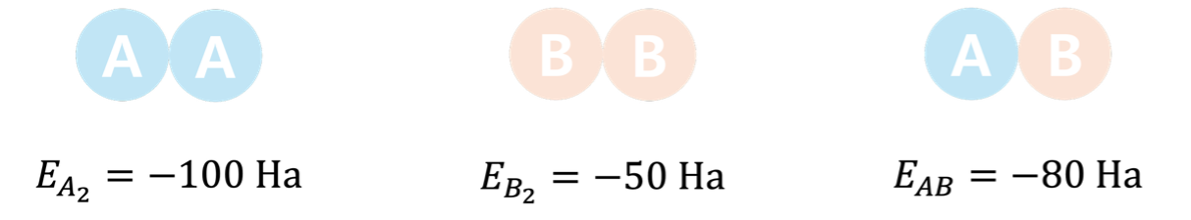
\includegraphics[width=0.8\textwidth]{fig/Eg예시.png}
  \caption{바닥상태 에너지 예시}
  \label{fig:example}
\end{figure}

위와같이 A\(_2\) 분자의 바닥상태 에너지는 -100 Ha, B\(_2\) 분자의 바닥상태 에너지는 -50 Ha, AB 분자의 바닥상태 에너지는 -80 Ha 정도인 상황을 보자. 여기서 Ha는 아래와같은 에너지단위이다:

\[
1~Ha = m_e R_y^2 \quad \textit{where} \quad m_e: \text{mass of Electron}, \quad R_b: \text{Bohr Radius}
\]

이런 상황에서, 어떤 진공 박스에 A\(_2\) 분자 1개와 B\(_2\) 분자 1개를 넣었다고 해보자. 
여기서, 우리는 일반적으로 시스템은 더 안정화된다는 경향이 있다는 물리적인 직관을 갖고 있다. 
즉, 어떤 시스템이 있으면, 그 에너지는 더욱 낮아지려고할것이다.

그런데 여기서, A\(_2\), B\(_2\) 가 각각 단분자로 존재한다고 하면 그 시스템이 갖는 에너지는 -150 Ha 일것이다. 
그런데, A와 B가 만나서 AB를 만들면, 하나의 AB 분자가 갖는 에너지는 -80 Ha 가 된다. 
따라서  그 시스템이 갖는 에너지는 -160 Ha 일것이고, 에너지가 더 낮아지므로 이렇게 되는것이 더 안정적인 상태이다.
즉, 박스안에 두 A\(_2\), B\(_2\) 분자를 넣었을때 아마 두 분자는 결합하여 2개의 AB 분자가 될것이다. 

\[
A_2 + B_2 \rightarrow 2AB
\]
더 일반적으로 제약분야와같은 상황을 생각할때, 어떤 약을 투여했을때, 그 약이 어떤 부위에 작용할것인가, 또 붙어서 어떤 반응을 작용할것인가 등의 현상이 가장 중요한 고민사항 일것이다.
이는 물리학자의 시선에서 에너지의 관점으로 바라보면, 이러한 작용들이 결국 전체 계의 에너지가 낮아지는 방향으로 진행될것임을 알 수 있고,
따라서 바닥상태 에너지의 계산을 통해 이러한 작용들을 이해할 수 있을것이라는 기대를 가질 수 있다.

이러한 논리는 분명 엄밀하지 않다. 단순히 바닥상태 에너지만을 이용해서 화학 반응을 계산할 수 있는것은 아니다. 
하지만 그럼에도 바닥상태 에너지가 그 반응에 있어 중요한 물리량 중 하나라는것을 직관적으로는 이해할 수 있을것이다. 
더 엄밀하게는, Gibbs 자유에너지를 계산해야하는데, 이 계산에는 바닥상태에너지가 필요하다. 
또한 특히 배터리 분야에서 생각한다면, 최근의 배터리 분야의 최대목적은 배터리의 소형화이다. 
이는 1) 산업적인 측면에서 배터리의 물리적인 크기를 줄이는것은 경제적인 이점이 있고, 
2) 리튬, 혹은 배터리에 사용되는 코발트 등 희토류 원소들은 그 자체로 최근 전쟁의 원인이 될정도로 지구상에 매우 한정적인 재료이다. 
그러한 재료를 덜 사용하고 같은 성능을 낸다 라는것은 환경적인 이유에서도 큰 이점이 될 수 있다. 
이러한 맥락에서 중요한것이 바로 “에너지 밀도” 이다. 즉, 부피당, 혹은 리튬이온 하나당 얼만큼의 에너지를 저장할 수 있는가가 매우 중요한 상황인데,
 이 에너지 밀도의 계산에서 화합물들의 바닥상태에너지의 계산이 필요하다.


\section*{HIVQE의 등장배경}


지금까지의 이야기를 통해 바닥상태 에너지 계산은 현대산업에 있어서 매우 중요한 계산이라는것을 이해할 수 있었다. 그럼 그 바닥상태 에너지는 어떻게 계산한다는가? 중요한 이야기일것이어서 쉽게 쉬웠으면 좋게 명확하게 이야기하지도 않았을것이다.



\begin{enumerate}[label=\arabic*)]
\item {\Large \textbf{Analytic Solution}}

결국 바닥상태 에너지라는것은 그 시스템이 갖는 가장 낮은 에너지일것이고, 이는 분자이므로 이문제의 물리는 양자역학으로밖에 해결할수 없었겠으며, 
이러한 시스템의 에너지를 계산하는 문제는 단순하게 아래와같이 슈뢰딩거 방정식을 해결하여 얻을 수 있다. 

\[
\hat{H}|\Psi\rangle = E|\Psi\rangle \longrightarrow
\left\{
\begin{aligned}
|\Psi\rangle &= \sum_n a_n |\psi_n \rangle \\
E_n &= \langle \psi_n | H | \psi_n \rangle
\end{aligned}
\right.
\]
근데 이게 쉽냐 하면 절대로 쉽지않다.  
일단 헤밀토니안에 따라 달라지겠지만, 물리학에서의 에너지는 보통 어떤 위치나 운동량과 같은 Cannonical 한 물리량의 제곱에 해당하는 항으로 주어지게 되고, 
보통 그렇기 때문에 슈뢰딩거방정식은 비선형 미분방정식이 된다. 
분자도 아니고, 원자를 보자. 원자중에서 가장 간단한 원자는 수소원자일것이고 
수소원자에서 위에서 파동함수와 에너지를 계산해보면, 아래와같다.
\begin{align*}
\psi_{nlm}(r, \theta, \phi) &= R_{nl}(r) Y_l^m(\theta, \phi) \\
R_{nl}(r) &= N_{nl} \left(\frac{2r}{na_0}\right)^l e^{-\frac{r}{na_0}} L_{n-l-1}^{2l+1}\left(\frac{2r}{na_0}\right) \\
Y_l^m(\theta, \phi) &= N_{lm} P_l^m(\cos \theta) e^{im\phi} \\
E_n &= -\left(\frac{m_e e^4}{8 \varepsilon_0^2 h^2}\right) \frac{1}{n^2}
\end{align*}
위의 표현에서 n=1 일때를 찾아본다면, 수소원자의 바닥상태와 바닥상태 에너지를 얻을 수 있을것이다. 
수리물리학을 잘 공부했다면, 이렇게 표현되는것 자체는 복잡하긴 해도 받아들일 수 있을것이다. 
하지만 말하고자 하는 내용은 아주 복잡하다는것이다. 
실제로, 이렇게 슈뢰딩거 방정식을 풀어 해를 얻는것이 가능한것은, 수소, 혹은 수소와같이 최외곽 전자가 하나인 원자뿐이다. 
거기다 이건 단순히 “원자”의 이야기이다. 우리가 결국 풀고자 하는 문제는 분자에 관한 문제이다. 분자에 대해서도 마찬가지로 이러한 해석적인 방법으로는 해결할 수 없다. 
그래서 이러한 문제를 해결하기 위해, 물리학자들은 많은 방식들을 시도하였고, 그중의 한가지 방식을 소개하겠다. 그 방식이 이후 VQE에도 사용될것이다. 
\end{enumerate}

\begin{enumerate}[label=2)]
\item {\Large \textbf{Variational Method}}

우리가 마주하고 있는 문제는 아래와같은 슈뢰딩거방정식이다.

\[
\hat{H}|\Psi\rangle = E|\Psi\rangle
\]

그런데 여기서 $|\Psi\rangle$를 구하는 것이 어려워 $E$를 구할 수 없었다. 
그래서 이렇게 시도를 해보는것이다. $|\Psi\rangle$를 우리가 어떤 파라미터를 포함한 형태로 임의로 구성하는것이다. 
이때는, 풀고자하는 시스템의 파동함수와 유사한 파동함수를 택할수도 있고,
혹은 임의의 Hilbert 공간의 함수를 표현할 수 있는 complete한 (현실적으로는 Complete 할것이라고 기대되는) 함수를 이용해서 표현할 수 있다.

어떻게든 함수를 파라미터를 포함한 형태로 표현하게되면,
\[
E(\theta) = \langle \Psi(\theta) | H | \Psi(\theta) \rangle
\]

에너지를 계산할 수 있고, 그 에너지는 파라미터에 대해 Explicit 하게 표현이 된다. 
그렇게되면 그 파라미터에 대해서 최적화 하여 우리가 구성한 함수 내에서 표현될 수 있는 가장 낮은 에너지를 계산할 수 있다. 
이제 여기서 한가지 논리를 생각해볼 수 있다.

\begin{enumerate}[label=*]
\item  \textbf{그 에너지가 과연 합리적인가? 그렇게 계산하는게 무슨 의미인가?}

이에 대한 논리를 주는 것이 Variational Principle 이다.

\begin{tcolorbox}[enhanced, breakable, colback=gray!10, colframe=black, title=Definition: Variation Principle]

\[
\langle \Psi | \hat{H} | \Psi \rangle \geq E_{\text{ground}}
\]

즉, 어떻게 상태를 구성하여 기대값을 측정하더라도 그 기대값의 계산결과는 항상 $E_{\text{ground}}$보다 크다.

\end{tcolorbox}

\begin{mdframed}
\textit{proof.} \\
Observable인 $\hat{H}$ 연산자는 Hermitian 이다. Hermitian 연산자는 언제나 orthonormal한 basis를 가진다. 즉, 아래의 고유치 방정식을 만들 수 있고,
\[
\hat{H} |e_i \rangle = E_i |e_i \rangle, \quad \langle e_i | e_j \rangle = \delta_{ij}
\]
그 Hilbert space에 존재하는 임의의 상태를 basis를 이용하여 아래와같이 표현할 수 있다.
\[
|\Psi_{\text{arbitrary}}\rangle = \sum_i c_i |e_i\rangle \tag{1}
\]

그리고 각 고유상태는 정규화 되어있다고 하자.
\[
\langle \Psi | \Psi \rangle = 1
\]


위에서 정의한 임의의 상태를 이용해 해밀토니안의 기대값, 즉 에너지를 계산해보면 아래와같다.

\begin{align*}
E_\Psi &= \langle \Psi | \hat{H} | \Psi \rangle \\
&= \left\langle \sum_i c_i e_i \left| \hat{H} \right| \sum_j c_j e_j \right\rangle \\
&= \sum_{i} \sum_{j} c_i^* c_j \langle e_i | \hat{H} | e_j \rangle \\
&= \sum_{i} \sum_{j} c_i^* c_j \langle e_i | E_j e_j \rangle \\
&= \sum_{i} \sum_{j} c_i^* c_j E_j \langle e_i | e_j \rangle \\
&= \sum_{i} c_i^* c_i E_i \\
&= \sum_{i} |c_i|^2 E_i \tag{2}
\end{align*}

즉,
\[
E_\Psi = \sum_{i} |c_i|^2 E_i
\]

임의의 상태는 고유상태에 대한 선형결합으로 표현될것이다. 그리고 그 상태의 에너지를 계산해보게되면, 각 고유상태에 대응되는 에너지와 그 선형계수의 제곱의 가중치합을 갖고 얻을 수 있다.

편의상 인덱스를 아래와같이 주자.
\[
E_0 (= E_{\text{ground}}) < E_1 < E_2 < \cdots
\]

각 에너지는 각 고유상태에 대응되는 에너지이므로, 그럼 바닥상태는 자연스럽게 아래와같이 표현할 수 있을것이다.
\[
|\Psi_{\text{ground}}\rangle = c_0 | e_0 \rangle = 1 \cdot | e_0 \rangle
\]

이 내용을 가지고 아래의 식을 쳐다보자.
\[
|\Psi_{\text{arbitrary}}\rangle = \sum_i c_i | e_i \rangle
\]
\[
E_\Psi = \sum_{i} |c_i|^2 E_i
\]

바닥상태인 상태는 "유일(unique)"하게 아래의 조건을 만족한다.
\[
c_0=1, \quad c_1=0, \quad c_2=0, \quad \cdots, \quad c_i=0 \; (i \neq 0)
\]

0이 아닌 인덱스에 대한 에너지가 아래와같이 약속했으므로,
\[
E_0 (= E_{\text{ground}}) < E_1 < E_2 < \cdots
\]

따라서 그 외의 조건에서 일반적인 상태에 대한 에너지는 바닥상태에너지보다 크게된다.
\[
E_\Psi = \sum_i |c_i|^2 E_i \ge E_0
\]
\end{mdframed}
즉, Variational Method를 통해 계산된 에너지는 바닥상태 에너지를 Lower Bound로 가지게 된다. 
즉, Variational Method를 통해 계산된 에너지를 계속해서 에너지가 낮아지는 방향으로 최적화를 진행하게 되면, 결국 다다르게 되는 에너지는 특정 basis 에서 헤밀토니안이 가질 수 있는 Ground-state energy가 되게 된다. 

\end{enumerate}

이러한 Variational Method에대한 간단한 예제가 있고 이것에 대해 이해해보자. 

\begin{mdframed}
\underline{\textbf{Variational Method 예제 (Quantum Harmonic Oscillator)}}

Quantum Harmonic Oscillator 시스템에서의 헤밀토니안은 아래와같다. 
\[H = -\frac{\hbar^2}{2m}\frac{d^2}{dx^2} + \frac{1}{2}m\omega^2 x^2 \]
사실 이거 풀수 있긴한데, 풀 줄 모른다고 해보자. 그럼 우리의 논리대로라면, 그 모르는 파동함수를 우리가 잘 아는 어떤 함수의 꼴로 구성해야할것이다. 
이 "잘 아는" 함수로 Gaussian 을 사용해보자. 
\[
\psi(x) = Ae^{-bx^2}
\]
이때 A 는 정규화 조건을 통해 구할 수 있다. 
\begin{align*}
1 &= |\psi(x)|^2  \\
&= |A|^2 \int_{-\infty}^{\infty} Ae^{-2bx^2} \, dx \\
&= |A|^2 \sqrt{\frac{\pi}{2b}}
\end{align*}
\[
\longrightarrow A = \left(\frac{2b}{\pi}\right)^{\frac{1}{4}}
\]
그럼이제 파동함수는 아래와같이 쓸 수 있다. 
\[
\psi(b,x) = \left(\frac{2b}{\pi}\right)^{\frac{1}{4}}e^{-bx^2}
\]
그리고 이 상태에서 앞선 논리대로 임의의 파동함수(양자상태)에 대해서 기댓값을 측정하여, 
에너지를 파라미터 b에 대해 Explicit 하게 표현해보자.
\begin{align*}
E(b) &= \langle H \rangle \\
&= \langle T \rangle + \langle V \rangle \\
&=\langle \psi|T|\psi \rangle + \langle \psi|V|\psi \rangle \\
&=\frac{\hbar^2 b}{2m} + \frac{m\omega^2}{8b}
\end{align*}


이제 저 파동함수를 통해 기술되는 에너지의 최솟값을 얻기위해 b에 대해 미분하자(최적화 과정). 
\begin{align*}
\frac{d}{db} E &= \frac{\hbar^2}{2m} - \frac{m \omega^2}{8b^2} \\
&\Longrightarrow b_0 = \frac{m\omega}{2\hbar}
\end{align*}

따라서 최적화된 파라미터를 에너지에 대입하면, 우리의 시험 파동함수(Ansatz)를 통해 기술되는 에너지의 최솟값을 계산할 수 있다. 
\[
E(b_0) = \frac{1}{2}\hbar\omega
\]
\[
cf, \quad E_{Analytic} = \frac{1}{2}\hbar\omega
\]
\end{mdframed}
이경우는 우리가 파동함수의 형태를 "우연히" 잘 잡아서 Exact 한 해와 같은 형태로 기술된다. 
이때, 저 함수의 형태를 어떤식으로 잡던지 저 값보다 작은 값은 얻을 수 없다(due to Variational Principle)
다른 시스템에서도 이처럼, 파동함수를 잘 기술하면 바닥상태 에너지에 가까운 에너지를 얻을 수있다. 
이런식으로 에너지를 계산하는것이 Variational Method 이다. 

자 그런데, 일반적으로, 파동함수을 단순하게 Gaussian 하나만으로 만들지는 않을것이다. 
예를들어 N개의 함수의 선형결합이라고 해보자. 
그러면, 이방식으로 문제를 진행하려면 결국 \(\langle H \rangle \\\)를 계산해야한다. 그리고 이때 총 적분해야할 항은 \(N^2\)개가 되게된다. 
우리가 결국 풀고자하는 분자의 시스템에서의 헤밀토니안은 쿨롱퍼텐셜항에 의해 \(\frac{1}{r}\)항이 생기게되고, 당연히 적분구간은 \(0~\infty\) 이다. 
이때 저 0이라는 구간때문에, 에너지가 발산해버리게되어서, 일반적으로는 적분이 안되고 수학적인 트릭들을 사용해야하는데, 이때 이러한 적분이 코스트가 크다. 
또, 일반적으로 저 N개를 택할때 몇억, 몇십억개의 basis를 사용하게되어 실질적으로 계산이 어렵다. 
따라서 이를 해결하기 위해 저 적분계산을 좀 쉽게 할수있는 방법이 없을까? 에대한 맥락에서 저 적분계산을 양자컴퓨터에서 돌려보자 라는 아이디어를 적용한 방식이 바로 VQE(Variational Quantum Eigensolver)이다. 

\vspace{\baselineskip}
\end{enumerate}

\begin{enumerate}[label=3)]
\item {\Large \textbf{VQE(Variational Quantum Eigensolver)}}

이 섹션만 해도 하고싶은, 해야할 이야기가 산더미처럼 있지만, 이 노트에서 정리하고싶은 내용이 VQE는 아니기때문에 여기는 간단한 스토리정도만 요약해보겠다.([1] 참고.)
2) Variational Method 에서 3)VQE 로 넘어가는 과정에서, 그럼 우리가 해야할것은 결국 \(\langle \psi|H|\psi \rangle\)를 파라미터화된 형태로 구성하고, 양자컴퓨터에서 계산하는 방법을 찾는것이다. 
이과정을 크게 파트별로 \(\mathrm{i}\)) hamiltonian의 구성, \(\mathrm{ii}\))Ansatz의 구성, \(\mathrm{iii}\)) \(\langle \psi|H|\psi \rangle\)의 계산 의 순서로 이해해보자. 
\begin{enumerate}[label=\(\mathrm{i}\))]
\item {\(H\)\,\textbf{(hamiltonian)}}

\begin{figure}[htbp]
  \centering
  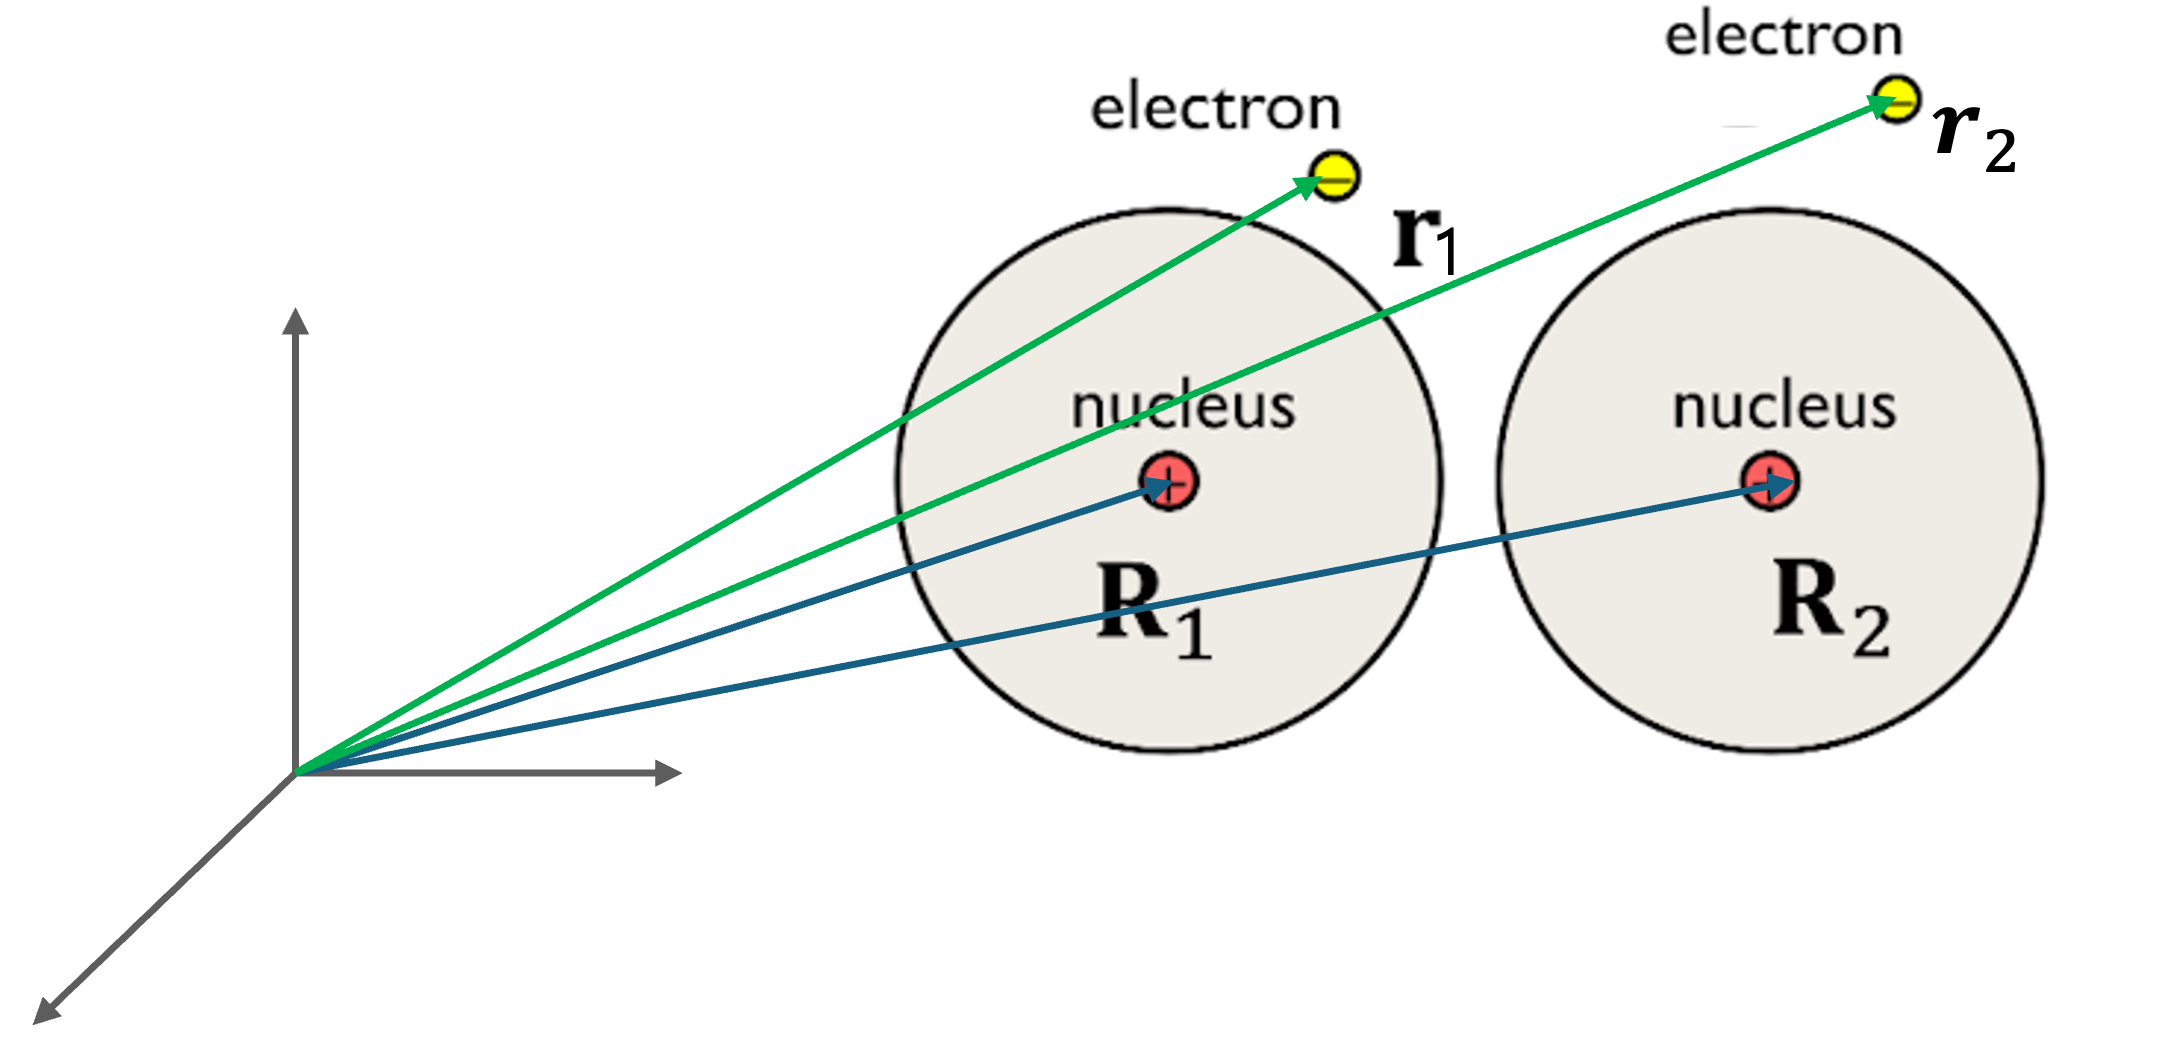
\includegraphics[width=0.5\textwidth]{fig/원자좌표.png}
  \caption{원자에서의 좌표 모식도}
  \label{fig:example2}
\end{figure}

그림 2와 같은 시스템을 보자. 여기서 고려 할 수 있는 헤밀토니안의 항은 아래와같다. 
\[
\hat{H}_{\text{elec}} = \hat{K}_{\text{atom}} + \hat{K}_{\text{elec}} 
+ \hat{V}_{\text{elec-nuclei}} + \hat{V}_{\text{elec-elec}} + \hat{V}_{\text{nuclei-nuclei}}
\]
그리고 각 항을 표현하면 아래와같이 표현된다. 
\[
\hat{H}_{\text{elec}} = - \sum_I \frac{\hbar^2}{2 M_I} \nabla_I^2
- \sum_i \frac{\hbar^2}{2 m_e} \nabla_i^2
- \frac{1}{2} \sum_{I,i} \frac{e^2}{4 \pi \epsilon_0} \frac{Z_I}{|\mathbf{r}_i - \mathbf{R}_I|}
- \frac{1}{2} \sum_{i \ne j} \frac{e^2}{4 \pi \epsilon_0} \frac{1}{|\mathbf{r}_i - \mathbf{r}_j|}
+ \frac{1}{2} \sum_{I,J} \frac{e^2}{4 \pi \epsilon_0} \frac{Z_I Z_J}{|\mathbf{R}_I - \mathbf{R}_J|}
\]

우선 여기에 \underline{a) Born-Oppenheimer 근사를 적용한다.} 
\begin{tcolorbox}[enhanced, breakable, colback=gray!10, colframe=black, title=Definition: Born-oppenheimer Approximation]


\begin{minipage}[t]{0.48\textwidth}
  \vspace*{0pt} % 그림을 minipage 맨 위로 올림
  \centering
  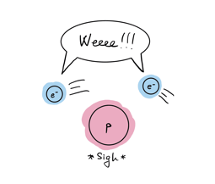
\includegraphics[width=\linewidth]{fig/BOapprox.png}
  \vspace{6pt}
  \textbf{Figure:} BO approximation diagram
\end{minipage}
\hfill
\begin{minipage}[t]{0.48\textwidth}
  \vspace*{10pt} % 텍스트도 minipage 맨 위로 정렬
  핵의 움직임이 전자에 비해 충분히 느려 핵의 움직임을 무시할 수 있다. 

\vspace*{8pt}

\(\rightarrow \mathbf{R}_I\) : Constant

\vspace{\baselineskip}

\(\rightarrow \sum_{i \ne j} \frac{e^2}{4 \pi \epsilon_0} \frac{1}{|\mathbf{r}_i - \mathbf{r}_j|} = 0\) 

\vspace{\baselineskip}

\(\rightarrow \sum_{I,J} \frac{e^2}{4 \pi \epsilon_0} \frac{Z_I Z_J}{|\mathbf{R}_I - \mathbf{R}_J|}\) : Constant

\vspace*{5pt}

(고유치 문제에서 상수는 고유벡터에 영향을 주지 않으므로 무시 하고 나중에 고려)

\end{minipage}

\end{tcolorbox}

이러한 근사방식은 분자계산에서 매우 합리적으로 받아들여지고 있고 이러한 근사를 적용하게되면 헤밀토니안은 아래와 같이 적을 수 있다. 
\[
\hat{H} = -\sum_i \frac{\hbar^2}{2 m_e}\nabla_{r_i}^2 -  \sum_I \sum_i \frac{e^2}{4\pi \epsilon_0}\frac{Z_I}{|\mathbf{r}_i-\mathbf{R}_I|}
+ \sum_i \sum_{j>i} \frac{e^2}{4\pi \epsilon_0} \frac{1}{|\mathbf{r}_i - \mathbf{r}_j|} + \cancelto{neglect! \, (in \,now)}{Const.}
\]

이 표현을 무차원변수로 만들어 주기 위해 \underline{b) atomic units 으로 표현하자.} 
\[Let.\quad r=\lambda r', \quad R=\lambda R'\]
여기서\(\lambda\) 를 Bohr Radius 로 잡게되면,
\[\lambda=\frac{4\pi\epsilon_0\hbar^2}{m_ee^2} (=\text{Bohr Radius})\]
헤밀토니안을 아래와같이 정리할 수있다. 
\begin{align*}
\hat{H} &= -\sum_i \frac{\hbar^2}{2 m_e{\color{red} {\lambda^2}}}\nabla_{r_i'}^2 -  \sum_I \sum_i \frac{e^2}{4\pi \epsilon_0{\color{red} {\lambda}}}\frac{Z_I}{|\mathbf{r'}_i-\mathbf{R'}_I|}
+ \sum_i \sum_{j>i} \frac{e^2}{4\pi \epsilon_0{\color{red} {\lambda}}} \frac{1}{|\mathbf{r'}_i - \mathbf{r'}_j|} \\
&=\left(\frac{m_ee^4}{16\pi^2\epsilon^2\hbar^2}\right)\left[-\sum_i \frac{1}{2}\nabla_{r_i}^2 -  \sum_I \sum_i \frac{Z_I}{|\mathbf{r}_i-\mathbf{R}_I|}
+ \sum_i \sum_{j>i} \frac{1}{|\mathbf{r}_i - \mathbf{r}_j|}\right]
\end{align*}
이러한 헤밀토니안으로 구성되는 슈뢰딩거방정식을 생각해보면 아래와같고. 
\begin{align*}
\hat{H}\vert\psi\rangle &= \left(\frac{m_ee^4}{16\pi^2\epsilon^2\hbar^2}\right)\left[-\sum_i \frac{1}{2}\nabla_{r_i}^2 -  \sum_I \sum_i \frac{Z_I}{|\mathbf{r}_i-\mathbf{R}_I|}
+ \sum_i \sum_{j>i} \frac{1}{|\mathbf{r}_i - \mathbf{r}_j|}\right]\vert\psi\rangle\\
&=E\vert\psi\rangle
\end{align*}
따라서 상수항을 에너지항으로 넘기면 아래와같이 정리할 수있다. 
\[
\left[-\sum_i \frac{1}{2}\nabla_{r_i}^2 -  \sum_I \sum_i \frac{Z_I}{|\mathbf{r}_i-\mathbf{R}_I|}
+ \sum_i \sum_{j>i} \frac{1}{|\mathbf{r}_i - \mathbf{r}_j|}\right]\vert\psi\rangle = {\color{blue}\left(\frac{16\pi^2\epsilon^2\hbar^2}{m_ee^4}\right)E} \vert\psi\rangle
\]

여기서 우변의 저 새로운 에너지를  단위 (or Atomic Unit) 에너지 라고 한다. 
\[
\left(\frac{16\pi^2\epsilon^2\hbar^2}{m_ee^4}\right)E[J] = E[Hartree]
\]


\(\left(\frac{16\pi^2\epsilon^2\hbar^2}{m_ee^4}\right)\) 는 계산해보면 \(1/E\)의 차원을 가지므로 우변 또한 무차원 변수로 표현되게 된다. 

여기에 우리가 풀 시스템이 전자(Fermion)로 구성되어있고, 그 시스템이 오비탈에 의해 양자화 되어있다는 사실에 착안하여, 생성/소멸 연산자를 정의하여 아래와같이 Second Quantized 된 형태로 표현할 수있다. 
\[
\hat{H} = \sum_{p,q} h_{pq} \hat{a}_p^\dagger \hat{a}_q
+ \frac{1}{2} \sum_{p,q,r,s} h_{pqrs} \hat{a}_p^\dagger \hat{a}_q^\dagger \hat{a}_r \hat{a}_s
\]

그리고 여기에 각 생성/소멸 연산자를 파울리 연산자로표현하는 Mapping(Jordan-Wigner, parity,...)을 사용하여 아래와같이 파울리 연산자(정확히는 파울리 스트링)의 형태로 표현할 수 있다. 
\[
\hat{H} = \sum_{a} \omega_a P_a, \quad \text{where} \quad
P_a = \hat{p}_0 \otimes \hat{p}_1 \otimes \cdots \otimes \hat{p}_N, \quad
\hat{p}_i \in \{I, X, Y, Z\}
\]

긴 과정을 거쳤지만, 결국 우리가 한것은 r이라는 변수로 표현되었던 헤밀토니안을, 파울리 연산자를 통해 표현하였고, 이 헤밀토니안이 이후 계산에서 사용될것이다. 

\end{enumerate}

\begin{enumerate}[label=\(\mathrm{ii}\))]
\item {Ansatz}


결국 여기서 해야할것은, 파라미터를 통해 표현된 양자상태 특히 VQE에서는 양자회로를 만들어야한다. 
그러기위해 생각할수 있는 두가지의 방법이 있을것이다. 

첫째는, 정말로 양자컴퓨터에서 임의의 양자상태를 만드는것이다. 따라서 이는 Hardware-Efficient 한 방법일것이다. 

\begin{figure}[H]
  \centering
  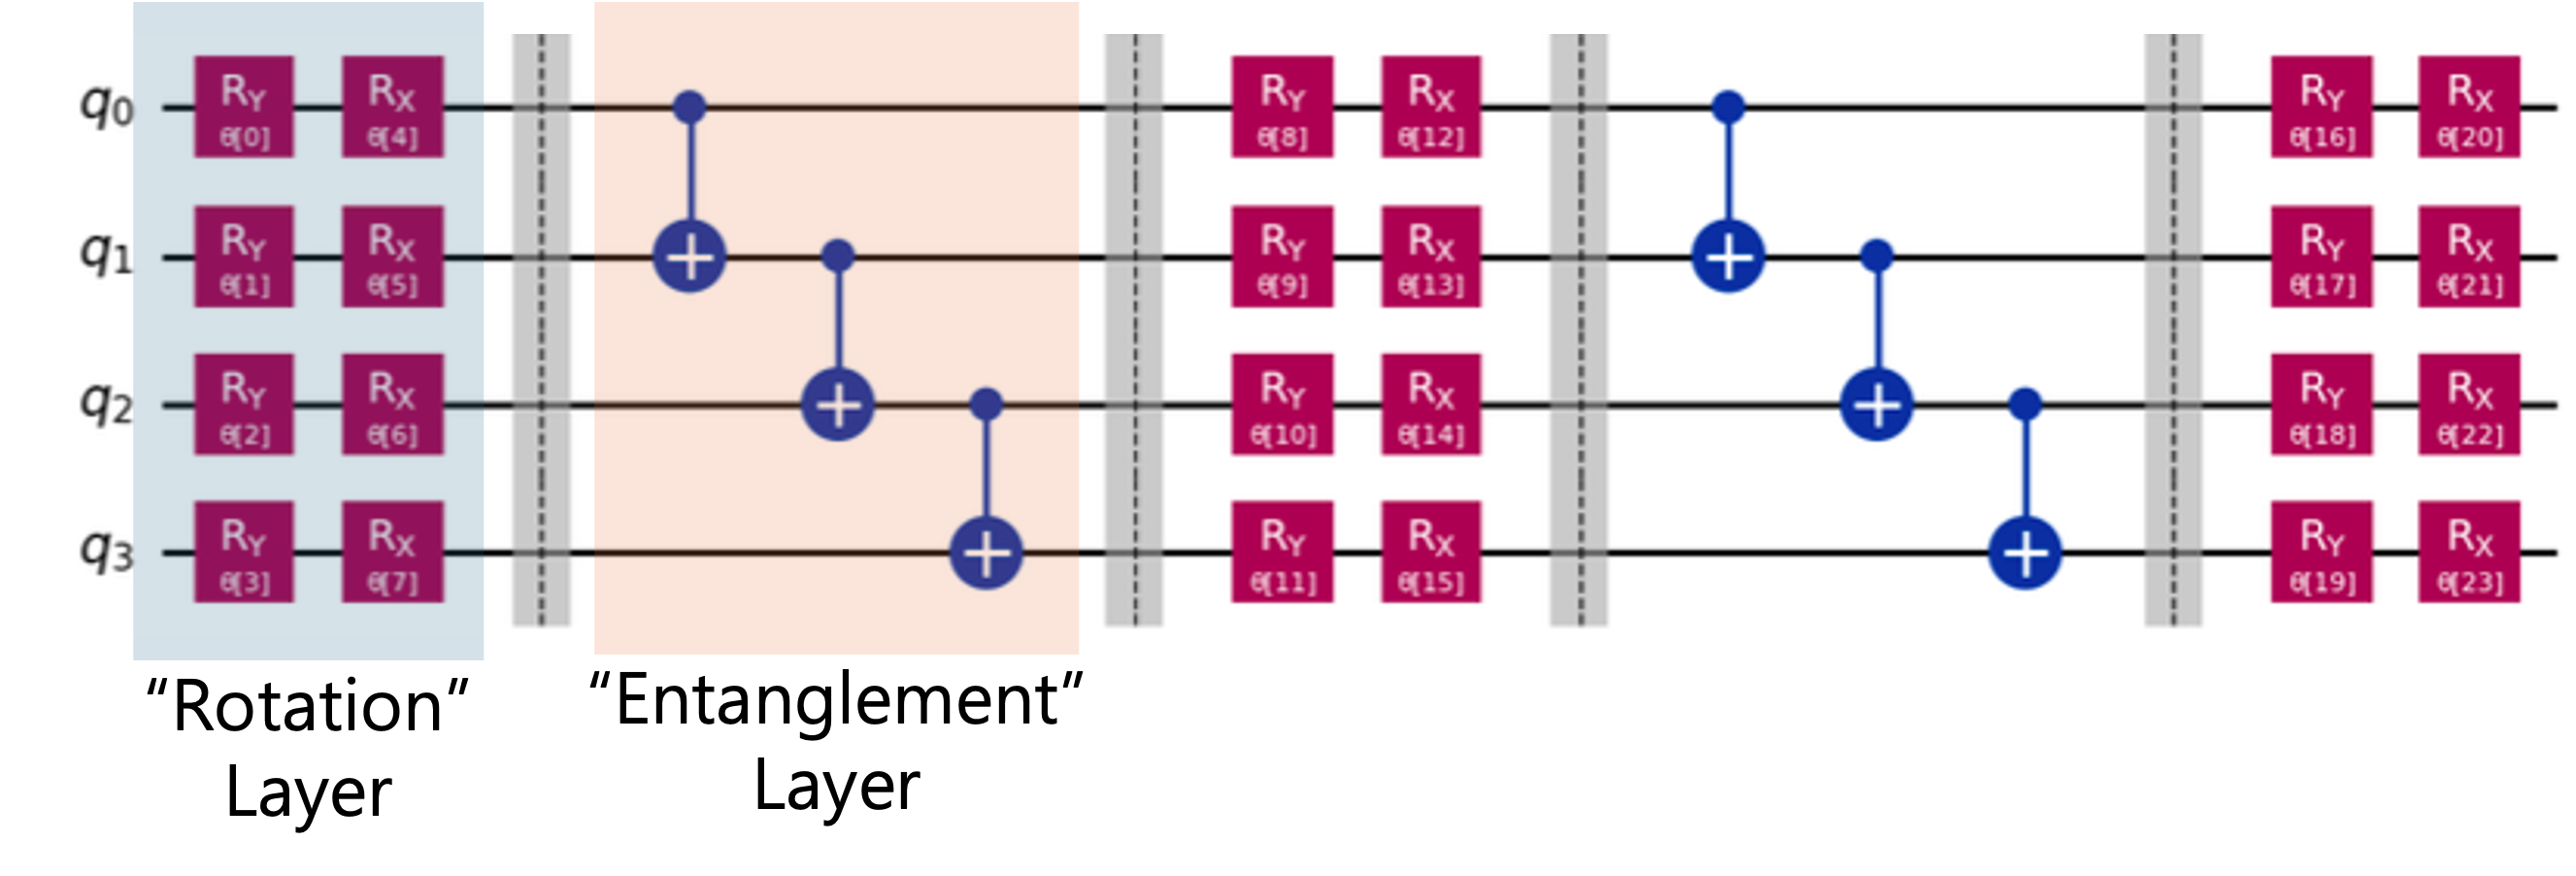
\includegraphics[width=0.8\textwidth]{fig/twolocal.png}
  \caption{twolocal Circuit}
  \label{fig:example3}
\end{figure}

임의의 single qubit의 양자상태는 두개의 Rotation Gate를 통해 만들 수 있다는점에 착안하여, 
두개의 Rotation Gate로 이루어진 Rotation Layer 와 Multi qubits 시스템이 갖는 특징인 Entanglement 를 CNOT 게이트로 구성된 Entanglement Layer를 번갈아여 구성하여
임의의 양자상태를 Rotation Gate의 각도를 파라미터로하여 표현하도록 하는 Ansatz이다. 이러한 Ansatz를 twolocal 혹은 Efficient SU2 라고 한다. 

둘째로는 문제에 조금더 특화된 Ansatz가 있을것이다. 기존의 양자화학계산인 FCI 에서의 계산방법에 착안하여
분자가 가질 수 있는 여러 Configuration들에 대응되는 Slater Determinant 를 basis로 양자상태를 표현한다. 
이때 각 Configuration은 어떤 기준상태로부터의 Excitation으로 기술 될 수 있으며, 따라서 각 Configuration은 생성/소멸 연산자로 표현될 수 있다. 
이렇게 문제에 맞는 헤밀토니안을 구성하고, 이를 파울리 게이트로써 Mapping 하게되면, 헤밀토니안에 잘 맞는 Ansatz를 구성할 수있으며, 이러한 형태의 Ansatz를 UCCSD Ansatz라고 한다. 
\end{enumerate}

\begin{enumerate}[label=\(\mathrm{iii}\))]
\item {에너지 계산}

우리가 계산해야할 것은, \(\langle \psi|H|\psi \rangle\) 이고, \(\mathrm{ii}, \mathrm{iii}\) 과정을 통해 임의의 파라미터화 된 양자상태(Ansatz)와 헤밀토니안을 구성하였다. 
우리가 가진 헤밀토니안의 형태는 \(\hat{H} = \sum_{a} \omega_a P_a\) 와 같고, 따라서 식을 아래와같이 정리 할 수있다. 
\begin{align*}
\langle \psi|H|\psi \rangle &= \langle \psi|\sum_{a} \omega_a P_a|\psi \rangle \\
&=\sum_{a} \omega_a \langle \psi|P_a|\psi \rangle
\end{align*}
여기서 하나의 \(P_a\) 에 대해서는 양자회로의 Projective Measurement 를 통해 그 기댓값을 계산하는것이 가능하다. 
따라서, Classical Optimizer를 통해서 계산된 값이 작아지도록 최적화 하면, 그 계산된 에너지가 VQE를 통해 계산된 에너지가 되고, 그 결과가 바닥상태에너지와 가까울 것이다.
\[
E_{VQE} =\min_\theta E(\theta) = \min_\theta \sum_{a} \omega_a \langle \psi(\theta)|P_a|\psi(\theta)\rangle
\]

\end{enumerate}
이런식으로 계산이 되는것이 VQE 알고리즘이다. 정말로 기존의 Variational Method 에서 기댓값 계산(에너지 계산) 부분만 양자컴퓨터로 바꿔치기 한 이야기 이다. 
이때, 각 양자컴퓨터에서 필요한 큐비트 수는 시스템의 스핀오비탈수와 같고, 따라서 QPE에 비해 필요한 큐비트가 적어 지금의 NISQ 시대에서도 효과적으로 사용할 수 있을것이라고 기대받고있고 많은 연구가 이루어지고있다. 
하지만 현재 이 방식에도 보완할 점이 있다. 우선, 에너지의 계산이 최적화과정에 의존한다는점이다. 최적화가 제대로 되지 않으면(실제로 제대로 잘 되지 않는다.) 에너지가 실제 이론값과 많은 차이를 보인다. 그리고, 위의 계산과정에서 보이는것처럼,
파울리스트링의 개수만큼 회로의 측정이 필요하다. 이는 시스템이 커질때마다 크게 증가하게된다. 

% Please add the following required packages to your document preamble:
% 
\begin{center}
\begin{tabular}{@{}ccccccc@{}}
\toprule
                   & \(H_2\) & LiH & \(H_2O\) & Co-O(single) & Co=O(Double) & LiCoO2((6,6),12)          \\ \midrule
\# of Pauli string & 15   & 631 & 1086  & 1545         & 2869         & \multicolumn{1}{c}{15017} \\ \bottomrule
\end{tabular}
\end{center}

이러한 특성들은 VQE를 실제 분자들에 적용하기 힘들게 만들기 때문에, 이를 해결하기위한 방법들이 연구가 되고있다. 지금부터 소개할 HI-VQE도 마찬가지로 이를 해결하기 위한 방법으로써 제시되었다.
\end{enumerate}
\newpage

\section{background}
HIVQE는 양자화학 계산중 하나인 SCI로 부터 아이디어를 얻은 알고리즘이며, 이 SCI는 FCI의 단점을 보완하기위해 제안된 알고리즘이다. 
따라서 HIVQE를 이해하기 위해서는 FCI등, 기존의 양자화학 계산은 어떻게 진행되는지 이해해야 수월할것이다. 따라서 그러한 내용을 먼저 다뤄보자. 

\subsection{How to Express \(|\psi \rangle\) ?}
FCI던 VQE 던 뭐든 계산하고자 하는것은 \(\langle \psi|H|\psi \rangle\) 이다. 이것을 얼마나 정확히,
그리고 효율적으로 계산할 수있는가가 여러 알고리즘들의 목적이 될것이다. 그리고 여기서 hamiltonian \(H\) 는 이미 알려져 있으니, 계산을 위해서는 우리가 보고자 하는 분자의 파동함수를 어떻게 기술하는지 알아야할것이다.
우리는 양자역학에서 배웠듯이, "원자" 에 대해서는 \(n,l,m\) 등의 양자수들로 표현되는 오비탈들의 결합으로 표현된다는것을 알고있다.
이러한 오비탈의 경우는 이해가 되온바가 있기때문에, 원자에 대해서는 파동함수를 표현할 수 있다. 하지만 분자의 경우는 그렇지 않다. 
여러 원자가 모여 분자를 형성하며 각 원자들의 오비탈이 섞여서 원자와는 다른 구조를 이루게 되고, 따라서 이는 우리가 이해하기 힘들다. 
그래서 분자의 파동함수를 어떻게 표현할것인가? 에 대한 논의를 이 섹션에서 정리해볼것이다.
이 논리의 흐름은 N차원 공간 \(S\)에서 N개의 직교벡터 \(\left\{b_i\right\}\)를 찾으면, 그 벡터집합\(\left\{b_i\right\}\)은 공간 \(S\)의 직교 basis가 됨을 이용해서, 
분자 파동함수가 있을 공간을 잘 정의하고, basis를 잘 찾는 과정이 될것이다. 

\subsubsection{Fermionic System}
우리는 지금 분자를 다루고 있고, hamiltonian의 형태를 보면 알 수있듯이, 전자의 좌표,성질 등에 의존하는 시스템을 다루고있다. 이 전자들은 어떤 대칭성을 갖고있으며, 이 대칭성은 우리가 파동함수를 다루는데에 있어서 중요한 열쇠가 될것이다. 

전자는, Identical particle이다. 그리고, 이러한 Identical한 입자가 갖는 성질은 이름 그대로 모든 입자들이 모두 똑같아서 구별 불가능(indistinguishable)하다는 것이다. 
그렇다는것은, 두개의 Identical한 입자가 있을때, 그 두개의 입자의 위치를 맞바꾸더라도, 우리가 보는 현상은 똑같아야 한다는것이다. 
이를 조금더 수식적으로 이해해보자. i,j 번째 입자의 위치를 맞바꾸는 연산자인 \(\mathbb{P}_{ij}\) 연산자를 생각해보며 아래의 시스템을 보자. 

\begin{figure}[htbp]
  \centering
  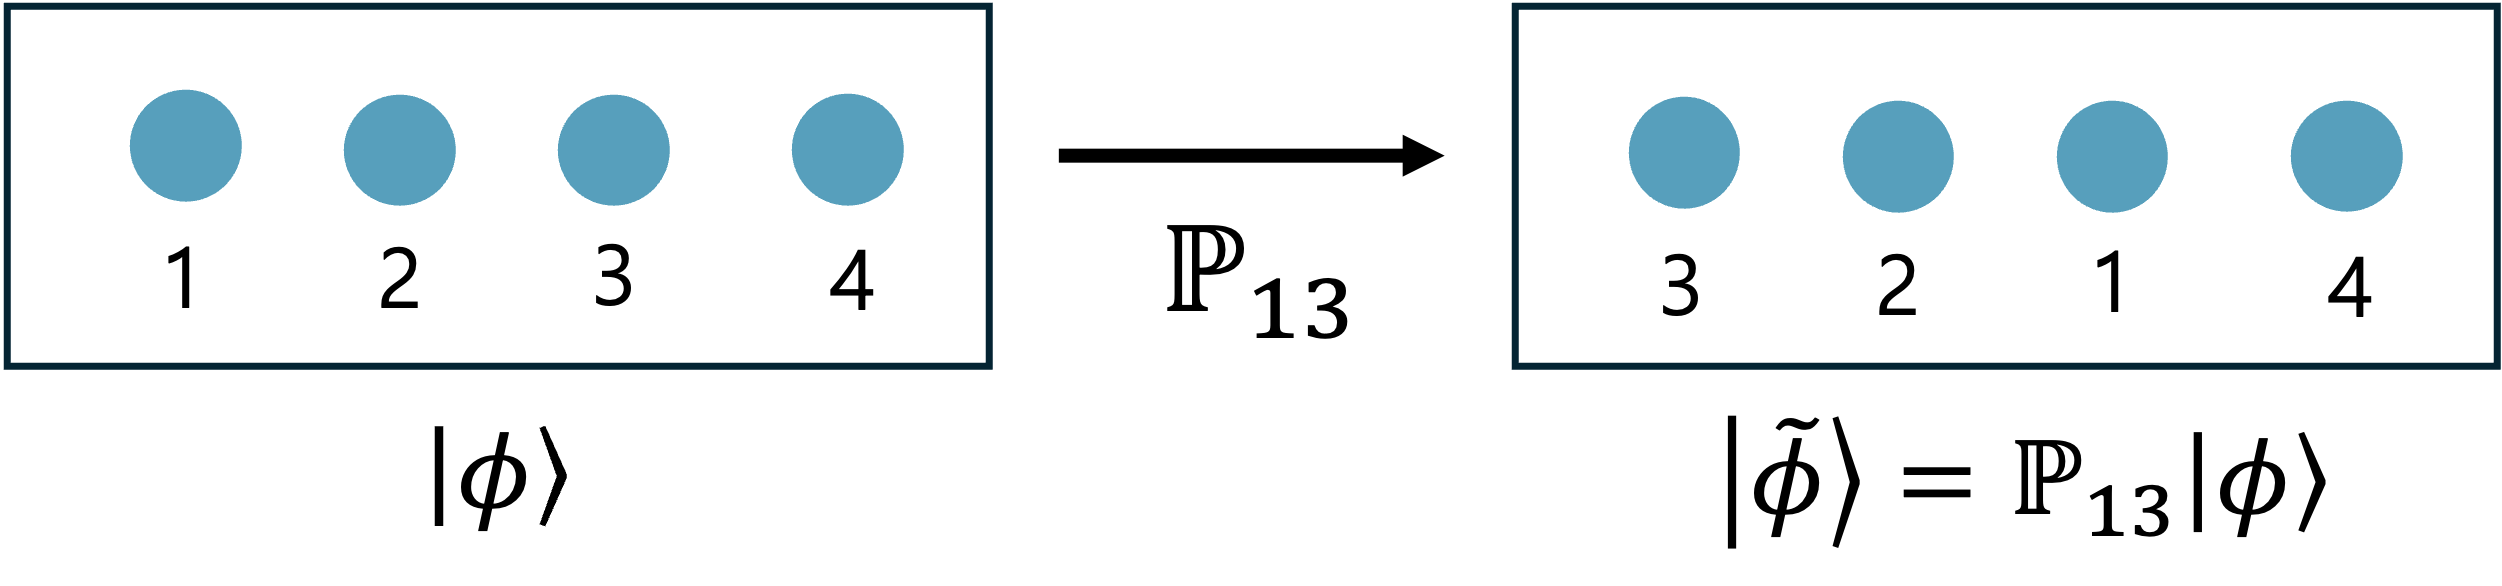
\includegraphics[width=0.8\textwidth]{fig/ident.png}
  \caption{System of Identical Particles}
  \label{fig:example2}
\end{figure}
\(\vert \tilde{\phi} \rangle\) 와 \(\vert \phi \rangle\)는 Identical particle 이므로 물리적으로 같은 현상을 기술해야한다. 즉, 같은 확률분포를 가져야한다. 따라서 아래와같이 쓸 수 있다. 
\begin{align*}
\mathbb{P}_{ij}\vert \phi \rangle &= \vert \tilde{\phi} \rangle \\
&= \lambda \vert \phi \rangle,\quad (\lambda \in \mathbb{C})
\end{align*}
즉, \(\lambda\)는 \(\vert \phi \rangle\)의 basis 에서 \(\mathbb{P}_{ij}\)  의 고유값이 된다. 

여기서 \(\vert \tilde{\phi} \rangle\)에 대해서 같은 인덱스의 \(\mathbb{P}_{ij}\) 연산자를 가한다면, Identical particle의 정의에 의해 \(\vert \phi \rangle\)와 같아야한다. 
\[
\mathbb{P}_{13} \vert \tilde{\phi} \rangle = \vert \phi \rangle
\]
즉, 아래와같이 정리할 수 있고, 
\[
{\mathbb{P}_{13}}^2 \vert \phi \rangle = \vert \phi \rangle
\]
여기에 위의 \(\mathbb{P}_{ij}\)의 고유값에 대한 표현을 대입하면 아래와같이 정리할 수있다. 
\[
{\lambda}^2 \vert \phi \rangle = \vert \phi \rangle
\]
\[
\longrightarrow {\lambda}^2 = 1
\]
\[
\longrightarrow \lambda = \pm 1
\]

정리해보면, Identical particle로 이루어진 시스템에 대해서 두 입자의 위치를 서로 교환하는것은 실제 물리적인 현상은 완전히 같지만, 그 파동함수의 위상은 달라질 수 있고, 
그때의 위상이 +1인 경우와 -1인 경우가 있다. 
이때 이 위상이 +1 인 입자를 Boson 이라고하고, -1인 입자를 Fermion 이라고 한다. 

\begin{figure}[htbp]
  \centering
  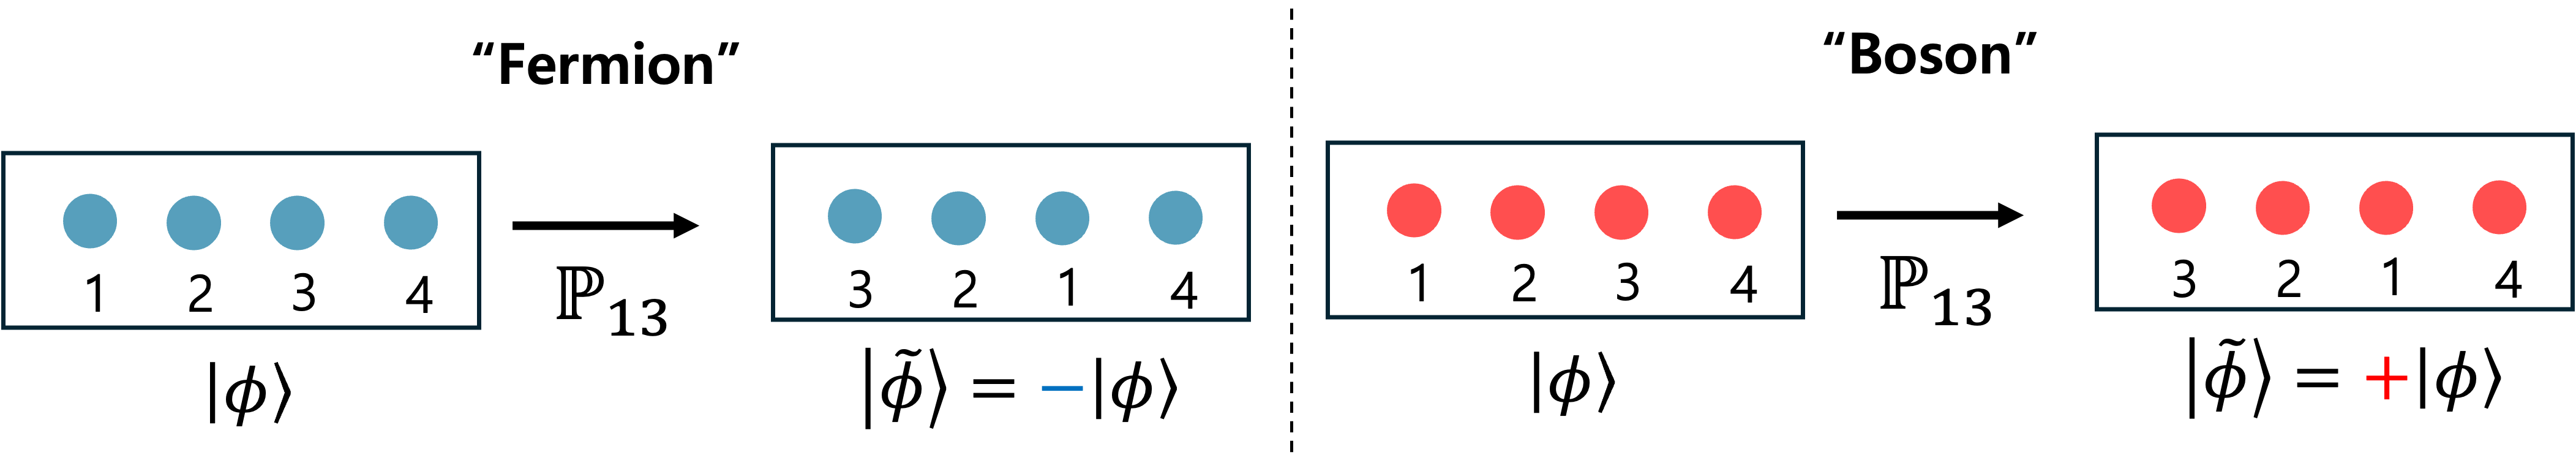
\includegraphics[width=0.9\textwidth]{fig/idet3.png}
  \caption{Bosons and Fermions}
  \label{fig:example2}
\end{figure}

우리가 다루는 시스템은 전자로 이루어져 있다고했고, 전자는 대표적인 Fermion 이다. 
즉, 우리가 구성해야할 파동함수는 전자에대한 정보(위치,스핀,...)들로 기술이 될텐데, 여기서 두 입자의 index를 바꾸는것에 대해서 시스템은 반대칭성을 가져야 한다는것을 알 수 있다. 
\[
\Psi_{fermion}(\dots, r_i, \dots, r_j, \dots) = -\Psi_{fermion}(\dots, r_j, \dots, r_i, \dots)
\]

\subsubsection{Slater Determinant}
이제 우리가 다룰것은 구체적으로 분자의 파동함수를 기술하고자 하는것이다. 그래서 어떤 형태일지 좀 구성을 해보자.
N-전자 파동함수에 대해서는 아래와같이 쓸 수 있다. 
\[
\Psi = \Psi(r_1, \dots, r_i, \dots, r_N)
\]
아러한 다변수함수를 다룰때, 물리학자들이 많이 하는접근은 모든 변수가 서로 독립인 상황을 보는것이다. 
물리적인상황으로는 각 전자들의 상호작용을 무시한다면, 아래와같이 적을 수 있다. (이러한 꼴로 표현하는것을  Product 라고한다.)
\[
\Psi(r_1, \dots, r_i, \dots, r_N)=\phi_1(r_1)\phi_2(r_2)\dots\phi_N(r_N)
\]
그런데 이러한 표현은 임의의 \(\phi_i\) 에 대해 입자들에 교환에 대해서 대칭이나 반대칭성을 부여하지 않는다. 
따라서 이러한 형태는 Identical particle 시스템을 다루기에는 적합하지 않다. 
임의의 \(\phi_i\) 에 대해서도 대칭성을 부여하기 위해서는 아래와같이 표현할 수 있다.
\begin{enumerate}[label=\(\mathrm{i}\))]
\item {\(N=2\)}
\[
\Psi(r_1,r_2)=\frac{1}{\sqrt{2}}[\phi_1(r_1)\phi_2(r_2)+\phi_1(r_2)\phi_2(r_1)],\quad (\text{bosonic System})
\]
\[
\Psi(r_1,r_2)=\frac{1}{\sqrt{2}}[\phi_1(r_1)\phi_2(r_2)-\phi_1(r_2)\phi_2(r_1)],\quad (\text{Fermionic System})
\]
\end{enumerate}
\begin{enumerate}[label=\(\mathrm{ii}\))]
\item {\(N=3\)}
\begin{align*}
\Psi(r_1,r_2,r_3)=\frac{1}{\sqrt{6}}&[\phi_1(r_1)\phi_2(r_2)\phi_3(r_3)+\phi_1(r_1)\phi_2(r_3)\phi_3(r_2) \\
&+\phi_1(r_2)\phi_2(r_1)\phi_3(r_3)+\phi_1(r_2)\phi_2(r_3)\phi_3(r_1)\\
&+\phi_1(r_3)\phi_2(r_1)\phi_3(r_2)+\phi_1(r_3)\phi_2(r_2)\phi_3(r_1)]\quad (\text{bosonic System})
\end{align*}
\begin{align*}
\Psi(r_1,r_2,r_3)=\frac{1}{\sqrt{6}}&[\phi_1(r_1)\phi_2(r_2)\phi_3(r_3)-\phi_1(r_1)\phi_2(r_3)\phi_3(r_2) \\
&-\phi_1(r_2)\phi_2(r_1)\phi_3(r_3)+\phi_1(r_2)\phi_2(r_3)\phi_3(r_1)\\
&+\phi_1(r_3)\phi_2(r_1)\phi_3(r_2)-\phi_1(r_3)\phi_2(r_2)\phi_3(r_1)]\quad (\text{Fermionic System})
\end{align*}
\end{enumerate}
우리가 볼것은 Fermionic System 이지만, 저 특성을 확인하기 위해 bosonic System도 같이 적었다. 
Fermionic System 의 파동함수에는 저렇게 -부호가 생기고, 이는 두 입자의 교환에 의해 생기는 위상이며, 이는 r에 붙어있는 인덱스들의 순열/역순열의 부호와 같다. 
반대로 Boson 에서는 입자교환에서 위상이 생기지 않기때문에, 모든 부호가 + 이다.
이러한 표현에서 N개 전자(Fermion)에 대한 임의의 표현을 적어보면 아래와같다. 

\[
\Psi(\mathbf{r}_1, \dots, \mathbf{r}_N) 
= \frac{1}{\sqrt{N!}} \det \begin{pmatrix}
\phi_1(\mathbf{r}_1) & \phi_2(\mathbf{r}_1) & \cdots & \phi_N(\mathbf{r}_1) \\
\phi_1(\mathbf{r}_2) & \phi_2(\mathbf{r}_2) & \cdots & \phi_N(\mathbf{r}_2) \\
\vdots & \vdots & \ddots & \vdots \\
\phi_1(\mathbf{r}_N) & \phi_2(\mathbf{r}_N) & \cdots & \phi_N(\mathbf{r}_N)
\end{pmatrix}
\]
\begin{center}
(Cf. Boson 에서는 Det 대신 perm 를 통해 기술할 수 있다.)
\end{center}

이렇게 행렬식의 꼴로 적으면, 시스템이 갖는 대칭성을 잘 부여할 수 있다는것을 이해했다. 이러한 꼴이 이제 Slater Determinant 로 이어질것이다. 
Slater Determinant 를 구성하기 위해서는 지금까지는 임의의 함수로 부여한 저 \(\phi\) 라는 친구가 어떤 꼴인지를 잘 정의하면 된다. 
\(\phi_i\) 라는 의미는 지금까지 \(i\) 번째 전자를 기술하기 위한 함수였다. 즉, \(i\) 번째 전자가 어떤 확률분포를 갖는지에 대한 정보, 즉 \(i\) 번째 전자의 파동함수에 대한 정보가 포함되어있어야한다. 
이러한 맥락에서 우리가 다루는 시스템은 지금까지는 "원자" 이고, 그 원자에서 어떤 전자들이 특정한 확률분포를 가지는것을 기술하기에 논리적으로 합당한것은 바로 "오비탈"이다. 
그래서 지금부터는 저 둘의 인덱스를 따로 부여하자. 
\[\phi_a(r_i)\]
이제부터는 이렇게 쓰고,이는 i번째 전자가 a오비탈을 점유한 상황을 나타낸다. 이거를 기반으로 아까 그 행렬식꼴을 다시쓴다면 아래와같다. 
\[
\Psi(\mathbf{r}_1, \dots, \mathbf{r}_N) 
= \frac{1}{\sqrt{N!}} \det \begin{pmatrix}
\phi_a(\mathbf{r}_1) & \phi_b(\mathbf{r}_1) & \cdots & \phi_M(\mathbf{r}_1) \\
\phi_a(\mathbf{r}_2) & \phi_b(\mathbf{r}_2) & \cdots & \phi_M(\mathbf{r}_2) \\
\vdots & \vdots & \ddots & \vdots \\
\phi_a(\mathbf{r}_N) & \phi_b(\mathbf{r}_N) & \cdots & \phi_M(\mathbf{r}_N)
\end{pmatrix}
\]
여기서, a,b,c 는 반드시 연속이지 않아도 된다. 
이거에대한 이야기는 조금더 뒤에 다루겠지만, M개의 오비탈이 있고, N개의 전자가 있다고할때, 일반적으로 M이 N보다 크다. 
그래서 그 오비탈들에게 1,2,3 이렇게 index 를 준다고 했을때, 분명 전자가 점유되지 않은 오비탈도 존재하게되고, 그 빈 오비탈은 고려되지 않기때문이다. 

이제 마지막 논리 이다. 그럼 저 오비탈이라고 한 \(\phi\)가 우리가 흔히 아는 1s, 2s, 2p 뭐 그런 오비탈들이냐? 하면 반은 맞고 반은 틀리다.
그렇게 파동함수를 기술하게되면, 예를들어 전자가 두개인 시스템을 다시 돌아가보자. 
\[
\Psi = \Psi(r_1,r_2)
\]

라고했는데, 
여기서 \(r_i\)라고하는것은 엄밀하게는 스핀까지 포함해야한다. 따라서 아래와같이 쓸 수 있다. 
\begin{align*}
r_i &= x_i s_i\\
x_i &: \text{Spartial coordinate of i-th Electron}\\
s_i &: \text{Spin coordinate of i-th Electron} \in \left\{-\frac{1}{2}, \frac{1}{2}\right\}
\end{align*}

따라서 
\begin{align*}
\Psi(r_1,r_2)&=\Psi(x_1,s_1, x_2,s_2)\\
&=\psi(x_1, x_2)\chi(s_1,s_2)
\end{align*}
와 같이 써지게 되고, 앞선 행렬식에서 \(\phi\)를 흔히 아는 오비탈로 택하면,이는 공간 Part 만을 다루는것이므로, 아래와같이 기술된다. 
\[
\Psi(x_1,s_1, x_2,s_2) = \frac{1}{\sqrt{2}}[\phi_1(r_1)\phi_2(r_2)-\phi_1(r_2)\phi_2(r_1)]\chi(s_1,s_2)
\]

이때, \(\frac{1}{\sqrt{2}}[\phi_1(r_1)\phi_2(r_2)-\phi_1(r_2)\phi_2(r_1)]\) 파트는 앞서 정의하기를 언제 Anti-Symmetry 하도록 구성을 하였다. 
따라서 전체 파동함수가 Anti-Symmetry 이려면 \(\chi(s_1,s_2)\) 이 파트는 Symmetry 여야만 한다. 
하지만, \(\chi(s_1,s_2)\)는 두개의 스핀의 덧셈이므로, 두전자의 스핀좌표가 같다면 스핀의 덧셈규칙에 의해 Singlet 상태또한 하나의 스핀상태가 되게 된다. 
여기서 Singlet 상태는 두 스핀의 교환에 대해서 Anti-Symmetry 하므로, 이경우에는 전체 파동함수(공간 + 스핀)이 입자의 교환에 대해 대칭인 함수가 된다. 
따라서, 이렇게 기술하는것은, 올바르게 시스템의 반대칭성을 기술할 수 없게된다. 
그래서 \(\phi\)는 아래와같이 Spartial-part 와 Spin-part 를 모두 기술하는 소위 스핀오비탈로써 택하게 된다. 
\[
\phi_a(r_i) = \psi(x_i)\chi(s_i)
\]

이렇게 기술하게되면, 
행렬식으로 표현된 파동함수가 전체 시스템을 기술하는 파동함수가 되어, spin과는 상관 없이 시스템의 반대칭성을 만족할 수 있다. 

이렇게 각 전자의 spin-orbital 파동함수를 이용하여, Anti-Symmetry를 만족하기 위해 행렬식의 꼴로 전체 시스템의 파동함수를 적은 꼴을 \enquote{\textbf{Slater Determinant}} 라고 한다. 
이 Determinant가 시스템이 만족해야할 성질들을 만족하는지 Check 해보자. 
\[
\Psi(\mathbf{r}_1, \dots, \mathbf{r}_N) 
= \frac{1}{\sqrt{N!}} \det \begin{pmatrix}
\phi_a(\mathbf{r}_1) & \phi_b(\mathbf{r}_1) & \cdots & \phi_M(\mathbf{r}_1) \\
\phi_a(\mathbf{r}_2) & \phi_b(\mathbf{r}_2) & \cdots & \phi_M(\mathbf{r}_2) \\
\vdots & \vdots & \ddots & \vdots \\
\phi_a(\mathbf{r}_N) & \phi_b(\mathbf{r}_N) & \cdots & \phi_M(\mathbf{r}_N)
\end{pmatrix}
\]


\begin{enumerate}[label=\(\mathrm{i}\))]
\item {Anti-Symmetry}

두 입자의 교환은 행렬식의 관점에서 r의 인덱스를 서로 맞바꾸는 것이고, 이는 행렬식에서 두개의 행을 바꾸는것과 같다.
그리고, 선형대수의 지식을 써먹어보면, 행렬식에서 두 행을 맞바꾸는것은 전체 행렬식에 - 부호를 붙히게 된다. 
\end{enumerate}

\begin{enumerate}[label=\(\mathrm{ii}\))]
\item {Pauli exclusive Principle}

파울리의 배타원리는, 한 오비탈에 같은 스핀전자가 두개 점유하는 경우는 물리적으로 옳지 않다 라는 내용이다. 
이거를 우리의 상황에 맞게 조금 언어를 바꿔보면, 한 스핀오비탈을 두개의 전자가 점유하는것은 물리적으로 옳지 않다. 라고 해석하면 된다. 
한 스핀오비탈을 두개의 전자가 점유하는것? 이건 phi 에 달려있는 index가 같은열이 있다는 소리이다. 
그리고 마찬가지로 선형대수의 지식을 끌어오면, 두 열이 같으면, 행렬식은 0이된다. 
즉, 파울리의 배타원리를 위배하도록 파동함수를 작성하면, 자동으로 파동함수는 0이된다. 
\end{enumerate}
이제 이러한 Slater Determinant를 일일히 적을 수 없으니 아래와같이 표현한다. 
\begin{align*}
\Psi(\mathbf{r}_1, \dots, \mathbf{r}_N) 
&= \frac{1}{\sqrt{N!}} \det \begin{pmatrix}
\phi_a(\mathbf{r}_1) & \phi_b(\mathbf{r}_1) & \cdots & \phi_M(\mathbf{r}_1) \\
\phi_a(\mathbf{r}_2) & \phi_b(\mathbf{r}_2) & \cdots & \phi_M(\mathbf{r}_2) \\
\vdots & \vdots & \ddots & \vdots \\
\phi_a(\mathbf{r}_N) & \phi_b(\mathbf{r}_N) & \cdots & \phi_M(\mathbf{r}_N) 
\end{pmatrix} \\
& \equiv \vert \phi_a \phi_b \dots \phi_M\rangle
\end{align*}
즉, 각 전자들이 점유한 오비탈을 통해 Determinant 를 표현할 수 있다. 



\subsubsection{Occupation number Representation}


Slater Determinant의 표현을 지금은 \enquote{어떤 전자가} 어떤 오비탈을 점유했는가를 통해 표현하고 있는데, 
사실 모든 전자는 Identical 하므로, 이를 \enquote{어떤 오비탈}이 전자가 점유 되었나 안되었나 만을 표기하면 될 것이라는 맥락에서 이렇게 표현을 바꿔보자는 것이다. 
이렇게 하면, 이전의 표현 \(\vert \phi_a \phi_b \dots \phi_M\rangle\)에서는 두 \(\phi\)를 바꾸는것이, 결국 전자 두개를 교환하는것 이므로, 상태 자체에서 Anti Symmetry를 갖게된다. 
하지만 미리 스포를 하자면, 이후의 설명에서는 모든 전자를 정말로 Identical 하게 보아, 상태에서는 전자의 교환이 정의 될 수 없고, 이러한 교환을 operator 로써 표현하여, 이 operator에 Anti Symmetry를 부여하여 시스템을 다루게 될것이다. 
이후 헤밀토니안도 이 basis에 맞춰 생성/소멸 연산자를 정의하여 헤밀토니안을 그 연산자를 통해 표현할것이다. 
이러한 과정을 Second Quantization 이라고 한다. 
\begin{figure}[H]
  \centering
  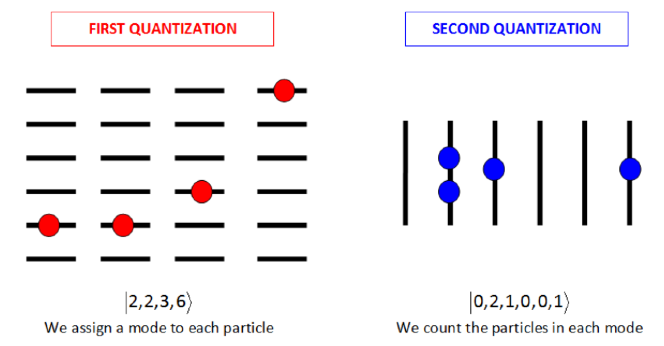
\includegraphics[width=0.7\textwidth]{fig/1to2.png}
  \caption{Second Quantization diagram}
  \label{fig:example2}
\end{figure}
그러기 위하여 아래와같이 number operator를 정의하자.
\[
\hat{n}_i : \text{number operator}
\]
여기서의 인덱스 \(i\)는 오비탈에 대응되는 인덱스 이다. 이 연산자의 형태는 이후 설명할것이고, 지금은 저 연산자의 역할을 이해해보자. 
이 연산자의 역할은 어떤 Slater Determinant 에 가해졌을때 i오비탈에 전자가 점유되었나 점유되지 않았나를 고윳값으로 반환한다. 즉, 아래와같이 표현된다. 
\[
\hat{n}_i | \Phi \rangle = n_i | \Phi \rangle, \quad n_i \in \{0,1\}
\]
그러면, 임의의 Slater Determinant를 number operator 의 고윳값을 통해 표현하면, 그 표현안에 전자에 대한 idex를 없앨 수 있다.
이부분은 구체적인 예시가 있는것이 이해하기 편할것 같아서 아래와같은 상황을 생각해보자. 

오비탈은 총 4개 이고, 각 index는 순서로 a,b,c,d 라고 하자. 

그리고 전자는 2개이고, a 오비탈과 c 오비탈을 점유하고 있다고 해보자. 

그렇다면, 기존의 Notation으로는 아래와같이 표기할 수 있다. 

\[| \Phi \rangle  = \vert \phi_a \phi_c \rangle\]

이러한 \(| \Phi \rangle\)에 대해서 이제 앞서 말했던것처럼 오비탈을 기준으로 표현하기 위해서, number operator \(\hat{n}_i\) 의 고윳값을 생각해보자. \(\hat{n}_i\)의 \(i\)는 오비탈에 대한 index 이므로, 
\(i \in \{a,b,c,d\}\) 일것이다. 이떄 전자가 점유되어있는 오비탈에 대해서는 \(\hat{n}_i\) 의 고유값이 1일것이고, 전자가 점유되어있지 않은 오비탈에 대해서는 \(\hat{n}_i\) 의 고유값이 0일것이다. 
즉, 
\begin{align*}
\hat{n}_a \vert \phi_a \phi_c \rangle\ = 1\vert \phi_a \phi_c \rangle\ &,\quad \hat{n}_b \vert \phi_a \phi_c \rangle\ = 0 \\
\hat{n}_c \vert \phi_a \phi_c \rangle\ = 1\vert \phi_a \phi_c \rangle\ &,\quad \hat{n}_d \vert \phi_a \phi_c \rangle\ = 0 
\end{align*}
그래서 이를 아래와같이 표현할 수 있다. 
\[| \Phi \rangle  = \vert \phi_a \phi_c \rangle = \vert 1010 \rangle  \] 

오른쪽과 같이 표현하는것을 Occupation number Representation 이라고하고, 이러한 표현은 이후 Second Quantized hamiltonian 과 계산할때 좀더 간편하게 계산할 수 있다. 
자 그러면, 이런 의문이 들 수 있다. \(\vert 1010 \rangle \) 이 표현은 이제 더이상 Anti Symmetric 하지 않은것인가? 왜냐면 이제 저기서는 전자를 교환한다는 아이디어를 적용할 수가 없는 표현이기 때문이다. 
이 의문을 해결하기 위해서는 number operator의 형태를 살펴보는것이 좋을것 같다. 
\[
\hat{n}_i = \hat{a}_i^{\dagger}\hat{a}_i
\]
이는 잘 아는 생성/소멸 연산자를 통해 기술되어있다. 이를 잠깐 Review 해보자면 아래와같이 Occupation number Representation 으로 표현된 오비탈에 대해 아래와같은 연산을 수행한다. 
\begin{align*}
\hat{a}_i^{\dagger} \vert 0 \rangle = \vert 1 \rangle_i &,\quad \hat{a}_i^{\dagger} \vert 1 \rangle_i = 0 \\
\hat{a}_i \vert 0 \rangle_i = 0 \quad &,\quad \hat{a}_i \vert 1 \rangle_i = \vert 0 \rangle_i
\end{align*}
생성연산자는 전자가 점유되어있지 않은 오비탈에 대해 전자를 생성하고, 이미 전자가 점유된 오비탈에 생성연산자를 가하면 0이된다. 
반대로, 소멸연산자는 전자가 점유되어있는 오비탈에 대해 전자를 없애고, 이미 점유되어있지 않은 오비탈에 소멸연산자를 가하면 0 이된다. 
그렇다면, 이제 어떤 Slater Determinant를 생성 연산자를 통해 표현할 수 있다. 
\begin{align*}
| \Phi \rangle = \vert 1010 \rangle &= \hat{a}_a^{\dagger}\hat{a}_c^{\dagger} \vert 0000 \rangle \\
&= \hat{a}_a^{\dagger}\hat{a}_c^{\dagger} \vert \rangle 
\end{align*}
\(\vert 0000 \rangle\) 는 전자가 하나도 없는 Vaccume State로 \(\vert \rangle\) 와같이 표기할 수 있다. 여기까지는 납득이 될텐데. 문제가 있다. 
\[
\hat{a}_a^{\dagger}\hat{a}_c^{\dagger} \vert \rangle \quad =? \quad \hat{a}_c^{\dagger}\hat{a}_a^{\dagger} \vert \rangle
\]
양 쪽의 표현 모두 a,c 오비탈에 전자를 생성하기때문에 \(\vert 1010 \rangle \)과 같은 상태를 만들것이다. 그럼 저 두 표현이 같은가? 하면 그렇지 않다. 
왜냐면 저 생성연산자는 아래와같은 Anti-commute relation을 만족한다. (소멸연산자가 만족하는 관계식 또한 적었다.)
\begin{align*}
\{ \hat{a}_p^\dagger, \hat{a}_q^\dagger \} &= 0 \\
\{ \hat{a}_p, \hat{a}_q \} &= 0 \\
\{ \hat{a}_p^\dagger, \hat{a}_q \} &= \delta_{pq}
\end{align*}
즉, 아래와같다. 
\[
\hat{a}_a^{\dagger}\hat{a}_c^{\dagger} \vert \rangle  = - \hat{a}_c^{\dagger}\hat{a}_a^{\dagger} \vert \rangle
\]
그렇다. 원래 System 이 가지고 있던 저 Anti-Symmetry를 저 연산자를 통해 표현한것이다. 그래서 하나의 순서를 기준으로 부호를 정의하자. 이는 결국 다른 Slater Determinant 들간에도 parity를 유지하기 때문에, 임의로 잡아도 되지만, 
가장 왼쪽부터 앞의 오비탈 index가 되도록 정렬하자. 이러한 Anti-Symmetry에 인해 생성/소멸 연산자가 가할때는 어떤 Parity가 생기게 된다. 
예를들어 \(\vert 1010 \rangle \) 여기에 b오비탈에 생성을 가하는경우와 d오비탈에 생성을 가하는 경우를 살펴보자. 

\begin{enumerate}[label=\(\mathrm{i}\))]
\item {b오비탈에 생성}

\begin{align*}
| \tilde{\Phi }\rangle & = \hat{a}_b^{\dagger}\vert 1010 \rangle \\
& = \hat{a}_b^{\dagger}\hat{a}_a^{\dagger}\hat{a}_c^{\dagger} \vert \rangle 
\end{align*}
그런데 우리는 여기서 두가지를 고려해야한다. 우선, 옳은 Parity 를 부여하기 위해서, 연산자들의 Index 를 오름차순으로 배열해야한다. 
그리고, 연산자의 순서를 바꿀때에는 Anti-Commute Relation을 고려해야한다. 
이를 만족시키기 위해서는 첫번째인 \(\hat{a}_b^{\dagger}\) 와 두번째에 있는 \(\hat{a}_a{\dagger}\)의 위치를 바꿔주어야 할것이다. 
그리고 한번의 위치교환에서는 -1의 부호가 생긴다 따라서 아래와같이 정리된다. 
\begin{align*}
| \tilde{\Phi }\rangle & = \hat{a}_b^{\dagger}\hat{a}_a^{\dagger}\hat{a}_c^{\dagger} \vert \rangle  \\
& = -\hat{a}_a^{\dagger}\hat{a}_b^{\dagger}\hat{a}_c^{\dagger} \vert \rangle \\
& = -\vert 1110 \rangle
\end{align*}
즉, -1의 부호가 생기면서 전자가 생성된다. 

\end{enumerate}

\begin{enumerate}[label=\(\mathrm{ii}\))]
\item {d오비탈에 생성}

\begin{align*}
| \tilde{\Phi }\rangle & = \hat{a}_d^{\dagger}\vert 1010 \rangle \\
& = \hat{a}_d^{\dagger}\hat{a}_a^{\dagger}\hat{a}_c^{\dagger} \vert \rangle 
\end{align*}
i) 에서와 마찬가지로 정리를 해보자. 

\begin{align*}
| \tilde{\Phi }\rangle & = \hat{a}_d^{\dagger}\hat{a}_a^{\dagger}\hat{a}_c^{\dagger} \vert\rangle \\
& = -\hat{a}_a^{\dagger}\hat{a}_d^{\dagger}\hat{a}_c^{\dagger} \vert \rangle \\
& = \hat{a}_a^{\dagger}\hat{a}_c^{\dagger}\hat{a}_d^{\dagger} \vert \rangle  \\
& = \vert 1011 \rangle
\end{align*}
이 경우에는 두번의 교환이 일어나 -부호가 사라져 + 부호가 되게 된다. 
\end{enumerate}
이를 일반적으로 표현하면 총 전자는 N개이고, 총 스핀오비탈은 M개가 있고, index는 a,b,...,M 순서로 있다고 할때, 임의의 i번째 오비탈에 연산자를 가하는 상황을, 
생성/소멸 연산자의 Anti-commute relation 을 고려하면 아래와같이 표현할 수 있다.
\begin{align*}
\hat{a}_i^{\dagger}\vert n_1 n_2 ,\dots, 0_i ,\dots n_M \rangle &= p_i \vert n_1 n_2 ,\dots, 1_i ,\dots n_M \rangle \\
\hat{a}_i^{\dagger}\vert n_1 n_2 ,\dots, 1_i ,\dots n_M \rangle &= 0 \\
\hat{a}_i\vert n_1 n_2 ,\dots, 1_i ,\dots n_M \rangle &= p_i \vert n_1 n_2 ,\dots, 0_i ,\dots n_M \rangle \\
\hat{a}_i\vert n_1 n_2 ,\dots, 0_i ,\dots n_M \rangle &= 0
\end{align*}

교환에 의해 생기는 Parity 를 \(p_i\) 라고 할때. 이는 아래와같이 정의된다. 
\[p_i = (-1)^{\sum_{j=a}^{i}n_j}\]
\(n=j\) 를 가지고 Parity를 세는 이유는, 상태를 연산자로써 표현할때, \(n_j=1\) 일때만, j번째 오비탈의 점유상태가 생성연산자로 표현될것이다. 
그리고, 우리가 실제 연산을 가할 i번째 오비탈에 대한 생성연산자를 오름차순으로 배열하려면, i번째 전에있는 생성연산자들과 교환을 총 \(\sum_{j=a}^{i}n_j\)해야하므로, 이와같은 Parity가 생긴다. 

이처럼, 작용하는 orbital에 따라 부호가 만들어 질 수 있다. 따라서 이러한 상황도 생각해 볼 수 있다.  \(\vert 1011 \rangle\) 로 바꾸는 상황을 생각할때 ii) 경우 처럼 만들수도 있지만, 
\(\vert 1001 \rangle\) 에 대해 c 오비탈에대한 생성연산자를 가하더라도 \(\vert 1011 \rangle\)상태가 만들어지겠지만 , \(\vert 1001 \rangle\)를 표현하기 위한 맨 앞의 a 오비탈에 대응되는 생성연산자와 
가해줄 c오비탈에 대응되는 생성연산자와의 교환에 의해 -1의 부호가 생겨 이경우는 \(-\vert 1011 \rangle\) 이 되게 된다. 
즉, 이렇게 생성/소멸 연산자를 다룰때에는 부호를 고려해주어야 한다는것을 주의해야한다. 

그럼 이제 number operator에 대해서 엄밀하게 이야기 해볼 수 있고, 그 정의는 아래와 같다. 
\[
\hat{n}_i = \hat{a}_i^{\dagger}\hat{a}_i
\]
이제 왜 이 형태가 왜 number operator의 역할을 수행하는지 느낌이 올것이다. 
연산자는 오른쪽에 있는게 먼저 작용하니, 우선 i오비탈에 소멸연산자를 가한다. 이때, Slater Determinant 의 i번째 오비탈이 전자가 점유되어있지 않다면, 그상태는 0이될것이고, 
이는 i번째 오비탈이 비어있는 경우이므로, number operator을 가했을때 0이 된다는것은 합리적이다. 
만약, Slater Determinant 의 i번째 오비탈이 전자가 점유되어있다면, i번째 오비탈은 1상태 일것이고 이 상태를 0으로 바꾼다. 
이때도 마찬가지로 앞서 얘기한 Parity가 생길것이다.

\begin{align*}
\hat{n}_i\vert n_1 n_2 ,\dots, 1_i ,\dots n_M \rangle &=\hat{a}_i^{\dagger}\hat{a}_i \vert n_1 n_2 ,\dots, 1_i ,\dots n_M \rangle \\
&= \hat{a}_i^{\dagger} p_i \vert n_1 n_2 ,\dots, 0_i ,\dots n_M \rangle
\end{align*}

\(p_i\)는 Scalar 이므로 앞으로 뺄 수있고, i번째 오비탈에 다시 생성연산자가 걸리므로 아래와같이 정리된다. 
\begin{align*}
\hat{n}_i\vert n_1 n_2 ,\dots, 1_i ,\dots n_M \rangle &=p_i \hat{a}_i^{\dagger}  \vert n_1 n_2 ,\dots, 0_i ,\dots n_M \rangle \\
&= (p_i)^2 \vert n_1 n_2 ,\dots, 1_i ,\dots n_M \rangle \\
&= (1) \vert n_1 n_2 ,\dots, 1_i ,\dots n_M \rangle
\end{align*}
즉, \(n_i = 1\) 일때, 다시말해 i 번째 오비탈이 점유해있을때만 고윳값이 1이되고, 그렇지 않은경우 0이된다. 
\begin{align*}
\hat{n}_i \vert \Phi \rangle &= \vert \Phi \rangle , \quad \text{(i-th orbital : occupied)}\\
\hat{n}_i \vert \Phi \rangle &= 0 , \quad \text{(i-th orbital : unoccupied)}
\end{align*}
그리고, 이러한 연산은 정확히 i번째 오비탈의 점유상태를 확인하고자했던 number operator의 목적에 부합한다. 


\subsubsection{Construct Molecular Wave Function}
자 이제 거의 다 왔다. 다시 우리가 하고자했던것을 되돌아보면 전체 시스템에 대해서 \(\langle \Psi|H|\Psi \rangle\)를 계산하고자 했던것이였고, 
여기서 \(|\Psi \rangle \)를 기술하기위해 지금까지 여러 논리들을 이어왔었다. 
잠시 Notation을 정리하고 가자. 
\begin{align*}
| \Psi \rangle &: \text{전체 시스템(분자)의 파동함수}\\
| \Phi \rangle &: \text{Slater Determinant}
\end{align*}
이제 분자의 시스템에 대해서 다뤄보자. 
간단하게 H2 의 시스템부터 가보자. 

\begin{figure}[htbp]
  \centering
  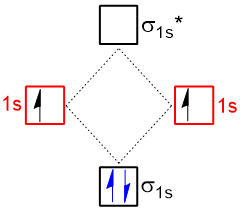
\includegraphics[width=0.4\textwidth]{fig/Moecular-Orbital-DiagramH2.png}
  \caption{H2 Molecular orbital diagram}
  \label{fig:example2}
\end{figure}

위의 그림이 잘 알려져있는 H2의 분자에서 오비탈이 어떤식으로 생성되는지를 보여주는 모식도 이다. 
빨간색으로 표시된것이 결합 전의 두개의 H 원자에 대한 오비탈의 모식도이다. 두 원자가 1s 오비탈을 각각 가지고 있을거고, 각 오비탈에는 전자 1개를 가지고 있다. 
그 두 원자가 결합하여 분자를 형성하며, 두개의 1s 오비탈은 파울리의 배타원리에 의해 같은 에너지를 가질 수 없으므로 Split 된다. 좀더 디테일하게는, 전자들의 스핀상태에 의해 에너지가 Split 되며, 
\(\sigma_{1s}\) 로 표시된 결합 오비탈이 Singlet 을 나타내며, \(\sigma_{1s}^*\) 로 표시된 반결합 오비탈이 Triplet 을 나타내게 된다. 그래서 반결합성 오비탈이 에너지가 더 높으므로, 그림에도 더 높게 그려져있다. 
이런식으로 가게될거라는건 정성적으로 이해하지만, 사실 \(\sigma_{1s}\) 의 함수의 형태가 어떤식인지는 알 수 없다. 
그래서 시스템의 파동함수를 \(\sigma_{1s},\sigma_{1s}^*\) 를 통해서는 기술 할 수 없고, 다른방식을 통해 기술해야하며, 그 방식이 바로 Slater Determinant를 이용하는것이다. 

가장 단순한 접근은 Slater Determinant 자체를 분자의 파동함수로써 사용하는것이다. 
하지만 하나의 시스템에서 Slater Determinant은 하나가 아니다. 
시스템이 M개의 스핀오비탈과 N개의 전자를 갖고있다면,  M개의 오비탈중 전자가 점유될 N개를 택하는 경우의수인 \(\binom{M}{N}\) 개의 Slater Determinant가 생기게 된다. 
여기서 M개의 오비탈중 N개의 전자가 점유된 하나의 그 상황을 Configuration이라고 하고, 그에 대응되는 Slater Determinant를 앞서 정의한대로 쓸 수 있다. 
여기서 각 Slater Determinant는 각 원자의 Spartial Part에 대응될 1s 오비탈의 파동함수와 Spin Part 에 대응될 \(Y^l_m\) 으로 그 형태를 적을 수 있고, 따라서 각 Determinant 에 대해 \(\langle \Phi_i|H|\Phi_i \rangle\) 를 계산 할 수 있다. 
모든 Slater Determinant 중, \(\langle \Phi_i|H|\Phi_i \rangle\) 값이 가장 작은 상태가 우리가 보고자 하는 바닥상태에 가장 가까운 상태일것이므로, 그 상태를 분자의 파동함수로 사용할 수도 있고, 
이러한 계산방법을 Hartree-Fock 계산 이라고 한다. 
하지만 이런 Hartree-Fock (HF) 계산은 정말 단순히 두개의 원자 오비탈만을 가지고 기술하는것이므로, 정확하지는 않다. 그래서 이러한 HF 계산보다 조금더 정밀한 계산을 필요로하고, 그러한 계산을 post-HF 계산이라고한다. 
이후 다루게될 모든 양자계산들은 이러한 Slater Determinant를 이용한 post-HF 계산이다. 
그래서 이러한 Slater Determinant를 가지고 전체 분자의 파동함수를 어떻게 기술할것인가? 가 관건인데, 여기에는 두가지 논리가 있다. 둘다 논리적으로 틀리지는 않지만, 두번째의 경우가 조금더 엄밀하다는 느낌이 있다. 

\begin{enumerate}[label=\(\mathrm{i}\))]
\item {Slater Determinant 집합이 Anti-symmetry Hilbert space 를 span 하는가? (추가 정리 필요)}

N개의 전자로 이루어진 시스템에 대해서, 각 전자의 정보 (위치,스핀,...)들의 좌표로 기술되는 함수로 구성되는 Hilbert Space \(\mathcal{H}_N\)이 있을것이고, 우리가 다루는 파동함수는 그러한 \(\mathcal{H}_N\) 에서 기술될것이다. 
그리고 \(\mathcal{H}_N\) 은 전자 한개에 대한 Hilbert space \(\mathcal{H}_1\) 의 N번의 텐서곱으로 표현될것이다. 
\[
\mathcal{H}_N = (\mathcal{H}_1)^{\otimes N}
\]
여기서,
\begin{align*}
\mathcal{H}_1 &=  L^2(\mathbb{R}^3 \times \{\uparrow, \downarrow\}) \\
L^2 (\left\{b\right\}) &: \left\{b\right\} \text{를 basis로 구성된 공간에서 제곱적분 가능한 함수의 공간} \\
\mathbb{R}^3 &: \text{전자 하나의 위치를 기술하기 위한 basis 집합}\\
\{\uparrow, \downarrow\} &: \text{전자 하나의 스핀을 기술하기 위한 basis 집합}
\end{align*}

그리고 이러한 \(L^2(\mathbb{R}^3 \times \{\uparrow, \downarrow\})\) 공간은 Spin orbital로 구성된 집합이 Span 한다 라는것이 알려져있다. 
(이부분 아직 모르곘음.,~Sturm–Liouville 정리..? )
무한하면 Complete하다 인데, 무한개가 있을 수 있나? Virtual 을 생각하는건가?? 
일단 넘어가자. 
아무튼 아래와 같이 정리 할 수 있고 
\[
\mathcal{H}_1^{(M)} := \text{span} \{ \varphi_1, \dots, \varphi_M \} \subset \mathcal{H}_1
\]
따라서 전체 시스템의 Hilbert space 는 아래와같이 쓸 수 있다 
\[
\mathcal{H}_N^{(M)} := \left( \mathcal{H}_1^{(M)} \right)^{\otimes N}
\]

하지만 이러한 표현은 Fermion의 Anti-Symmetry 가 고려되지 않은 공간이다. 이러한 Anti-Symmetry 를 만족하는 어떤 subspace \(\mathcal{H}_N^{anti}\)에 우리가 구성하고자 하는 파동함수가 있을것이다. 
\[
\vert \Psi \rangle \in \mathcal{H}_N^{anti} \subset \mathcal{H}_N
\]
이러한 \(\mathcal{H}_N^{anti}\)를 수학적으로 아래와같이 구성할 수 있다. 


\begin{align*}
\mathcal{H}_N^{\text{anti}} &= \bigwedge^N \mathcal{H}_1\\
&= \mathcal{H}_1 \wedge \mathcal{H}_1 \wedge \dots \wedge \mathcal{H}_1
\end{align*}

여기서, 
\[
\mathcal{A} := \frac{1}{N!} \sum_{\pi \in S_N} (-1)^{\text{sgn}(\pi)} \hat{P}_\pi
\]

\begin{center}
\textbf{\Large ~이후 추가 예정~}
\end{center}
\end{enumerate}

\subsection{FCI(Full Configuration Interaction)}
FCI에 관한 이야기를 다뤄보자. 그중에 FCI 는 모든 계산방법중 \(\langle \psi|H|\psi \rangle\)를 가장  \enquote{정확히} 계산하기 위한 계산방법이다. 
이 계산방식은 다른 양자화학 계산들의 기준값이 된다. (그니까 FCI 와 비교했을때 이만큼의 차이가 난다. 이런식으로) 그러한 FCI의 계산방법에 대해 이해해보자. 
헤밀토니안은 이미 Spin-orbital basis로 Second Quantization 의 형태로 구성이 되어있다. 따라서 계산방법(알고리즘) 의 정확도는, 상태를 얼마나 정확히 표현할것인가에 따르게된다. 
어떤 상태를 표현할 때 해당 상태가 있는 공간의 모든 basis의 선형결합을 통해 표현하는것이 가장 정확하다. 
그리고, 앞의 내용을 통해 Anti-Symmetric Hibert Space는 Slater Determinant 집합이 span 한다는것을 이해했다. 
따라서, 분자의 파동함수는 다음과 같이 모든 Slater Determinant를 basis로 표현하는것이 가장 정확한 표현이다. 
\[
|\Psi\rangle = \sum_I c_I |\Phi_I\rangle
\]
그리고 분자의 에너지계산에 이러한 모든 basis를 사용하여 표현된 파동함수를 사용하여 하는 계산이 바로 FCI 이다. 

자그럼 여기서 basis의 갯수? 혹은 저 함수가 표현되는 공간?에 관한 이야기를 잠깐 하고 실제 에너지 계산방법으로 넘어가보자. 
\subsubsection{Symmetric Space}
일단 이름이 썩 마음에 들지는 않지만, 이 논문에서 사용한 용어가 "Symmetric Space"이니 그대로 따라가보자. 
일단 Slater Determinant 를 Occupation number 표현으로 아래와같이 Binary String 으로 표현된다는 것은 앞선 섹션에서 이야기하였다. (N : 전자수, M : spin orbital 수)
\[\Phi_i = \vert n_1n_2,\dots n_M \rangle ,\quad n_i \in \{0,1\}\]
\[\sum_{i=0}^{M}n_i = N\]

이때, H2 분자에서의 FCI 계산을 보자.
H2 분자는 총 스핀오비탈 4개, 전자 2개인 시스템이다. 
따라서 비트스트링은 총 4개의 길이 일텐데, 그럼 이 계산에서 아래와같이 0000 ~ 1111 까지 모든 비트스트링에 대응되는 Slater Determinant를 고려해야할까? 

\begin{figure}[htbp]
  \centering
  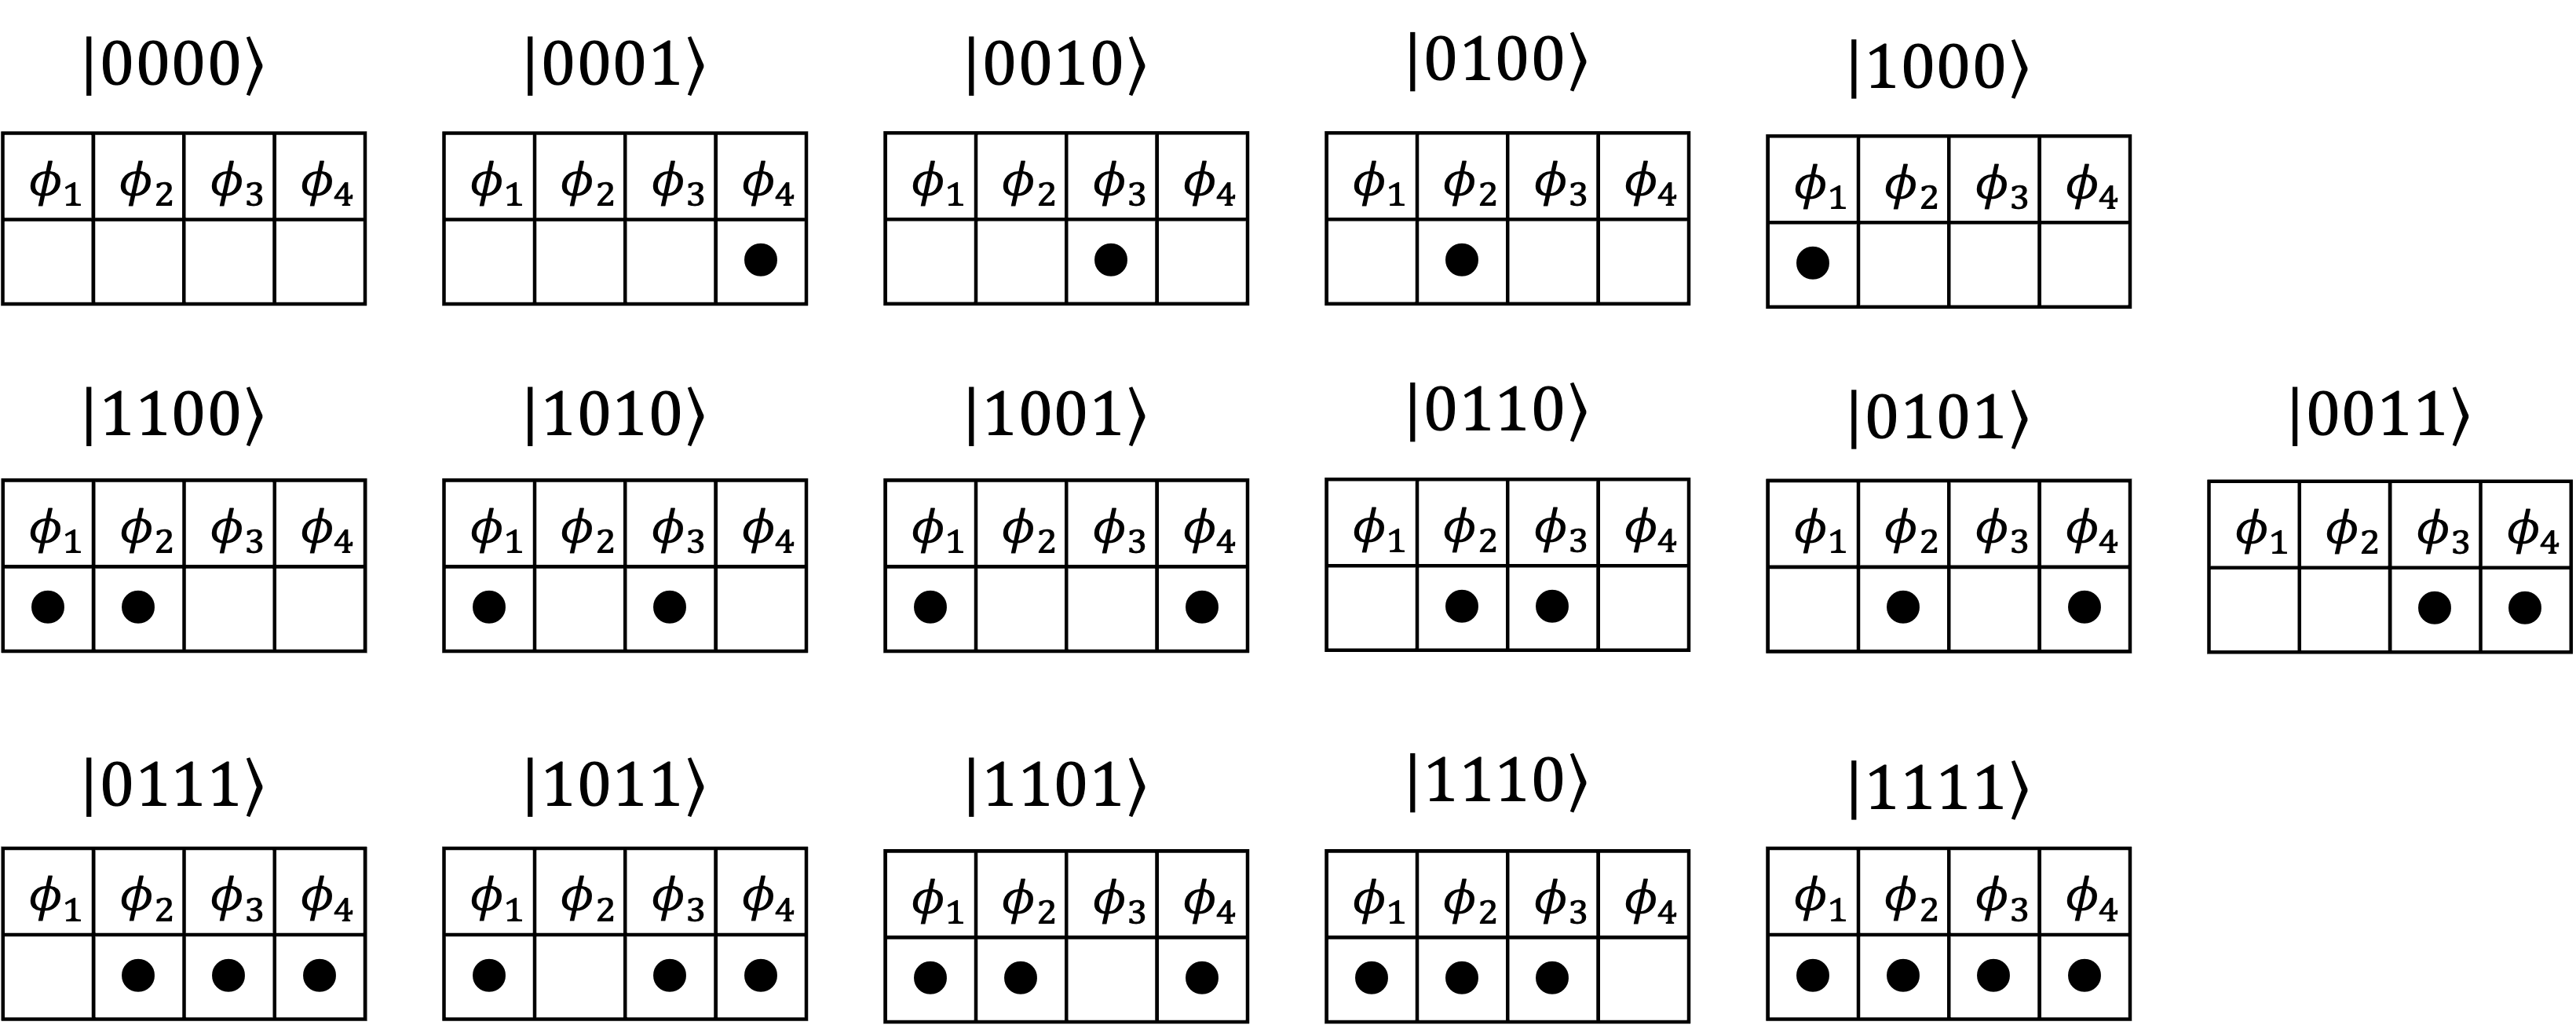
\includegraphics[width=0.8\textwidth]{fig/Cofig.png}
  \caption{all Slater Determinant of H2}
  \label{fig:example2}
\end{figure}

그림에서 표현되어있지만, Occupation number Representation 으로 표현된 상태에서 1은 해당 오비탈에 전자가 점유되어있음을 의미한다. 
그래서 스트링에서 총 1의 갯수는 해당 스트링이 나타내는 Configuration에서의 전자의 개수를 의미한다. 
그렇다면 우리가 다루고자 하는 시스템은 전자가 2개인 시스템이므로, 전자의 개수가 2가 아닌 스트링 , 즉 총 1의 개수가 2가 아닌 스트링은 우리가 다루는 시스템을 기술하기에 적합하지 않을것이다. 
그래서 이러한 Configuration에 대해서는 FCI 계산에서 고려하지 않는다. 
\begin{figure}[htbp]
  \centering
  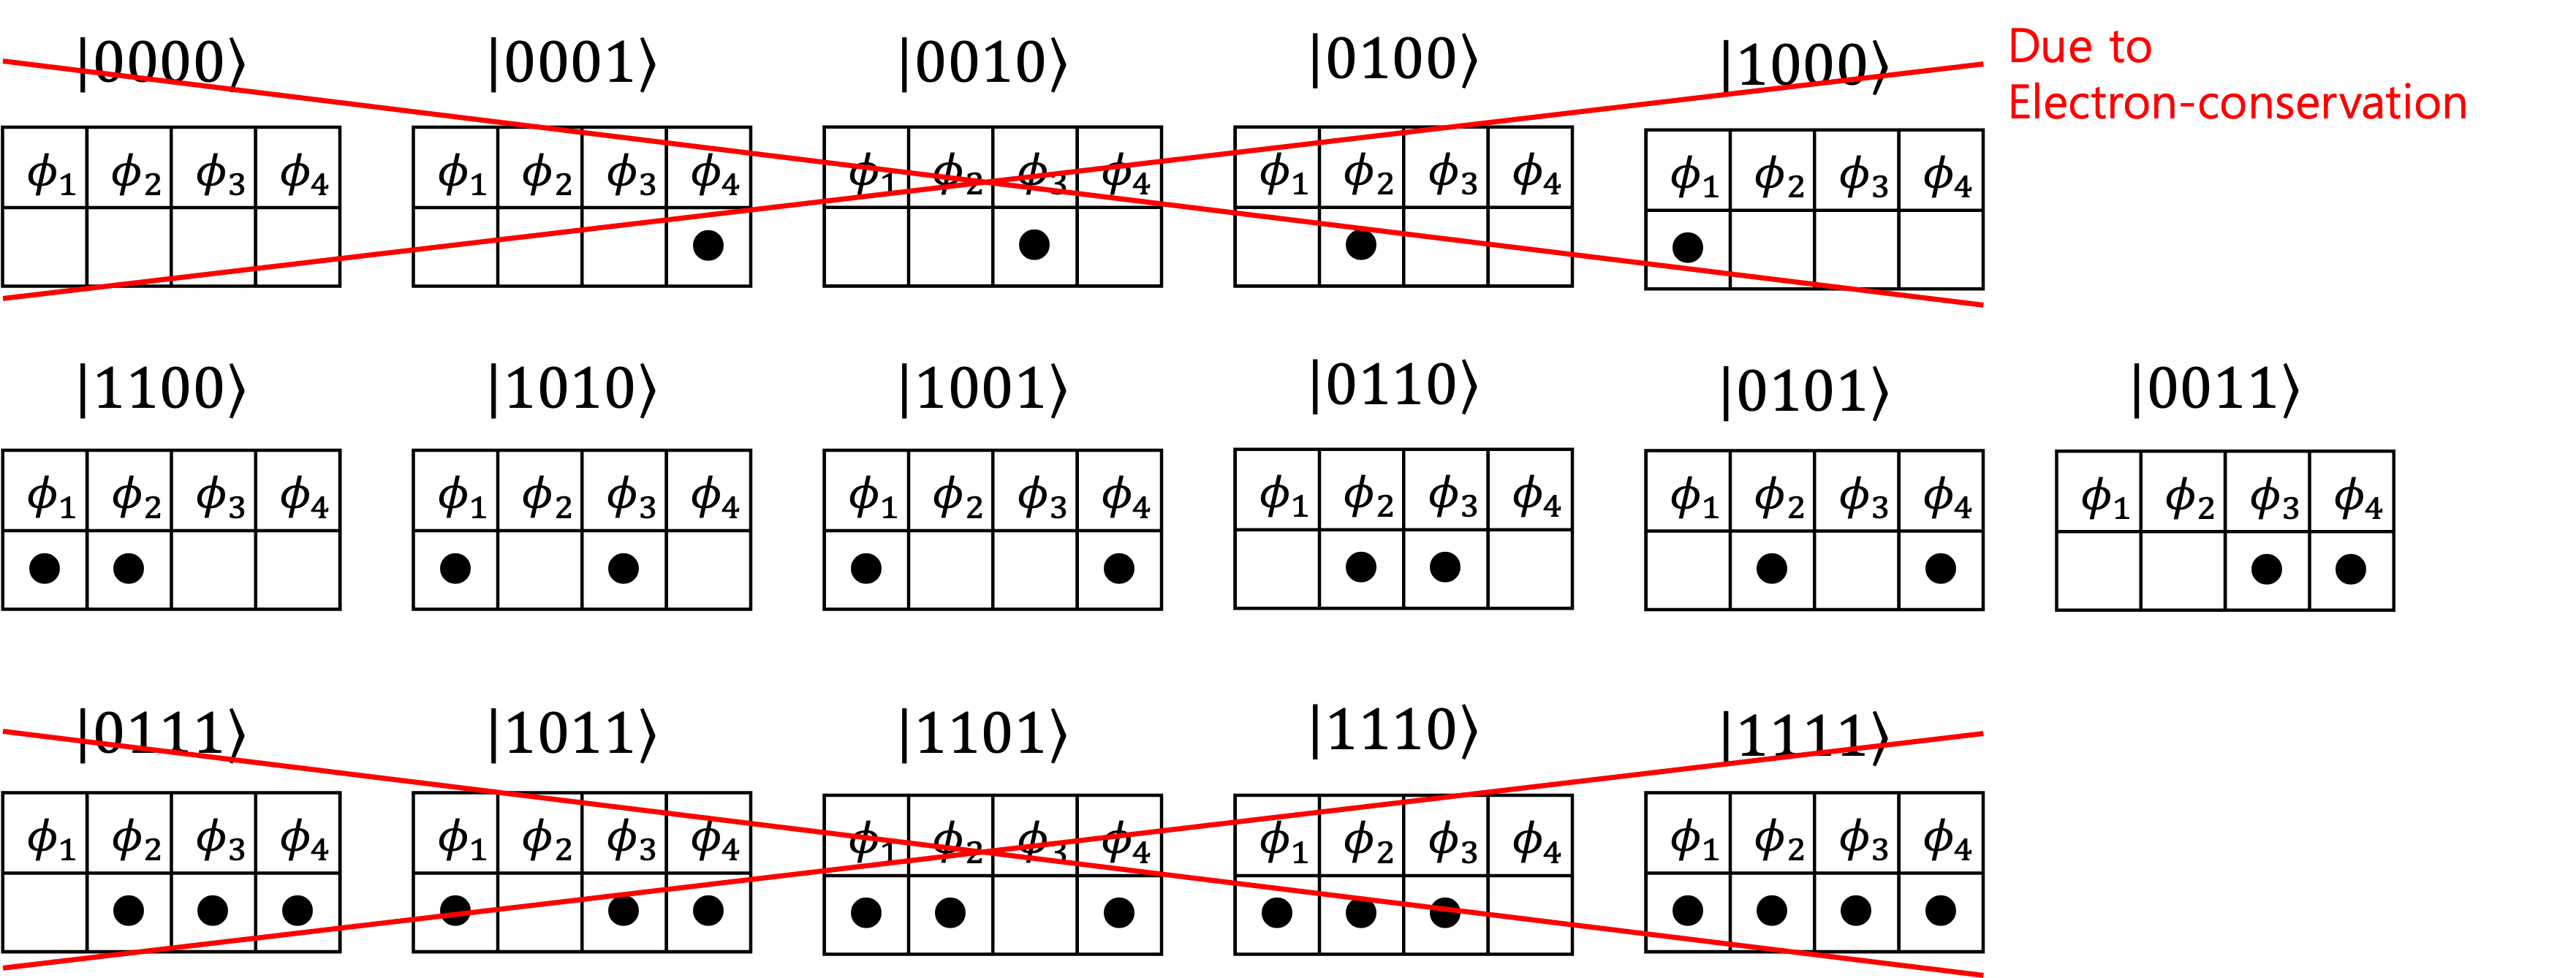
\includegraphics[width=0.8\textwidth]{fig/Elec_cons.png}
  \caption{Validate Determinant of H2}
  \label{fig:example2}
\end{figure}
여기에 우리가 다루는 오비탈이 스핀오비탈이라는점을 고려하면 몇개의 Slater Determinant를 추가로 지울 수 있다. 
스핀오비탈은 하나의 Spartial orbital 당 2개가 있다. 즉, 이는 up-spin 에 대응되는 오비탈과 down-spin에 대응되는 오비탈이 있다는 의미이고, 
이 계산에서 관습적으로 앞의 절반은 up-spin 에 대응되는 오비탈을 표기하고, 뒤의 절반은 down-spin 에 대응되는 오비탈로 표기한다. 즉 우리의 그림에서는,
\begin{align*}
\phi_1, \phi_2 &: \text{up-spin orbital} \\
\phi_3, \phi_4 &: \text{down-spin orbital}
\end{align*}
그렇다고 했을때, 우리는 총 시스템의 Multiplicity를 고려할 수 있다. 이는 시스템이 Singlet인지, Doublet 등등 인지에 대한 정보이며, 이는 분자를 구성하는 원자의 결합상태등에 의존하는 값이다. 
\(H_2\) 분자는 최외각 오비탈이 닫혀있는 결합을 취하므로, Singlet이 되며, 따라서 이경우 두 전자의 스핀이 모두 up 이거나, 모두 down 인 경우는 고려되지 않는다. 따라서 아래의 두 경우를 지울 수 있다. 
\begin{figure}[htbp]
  \centering
  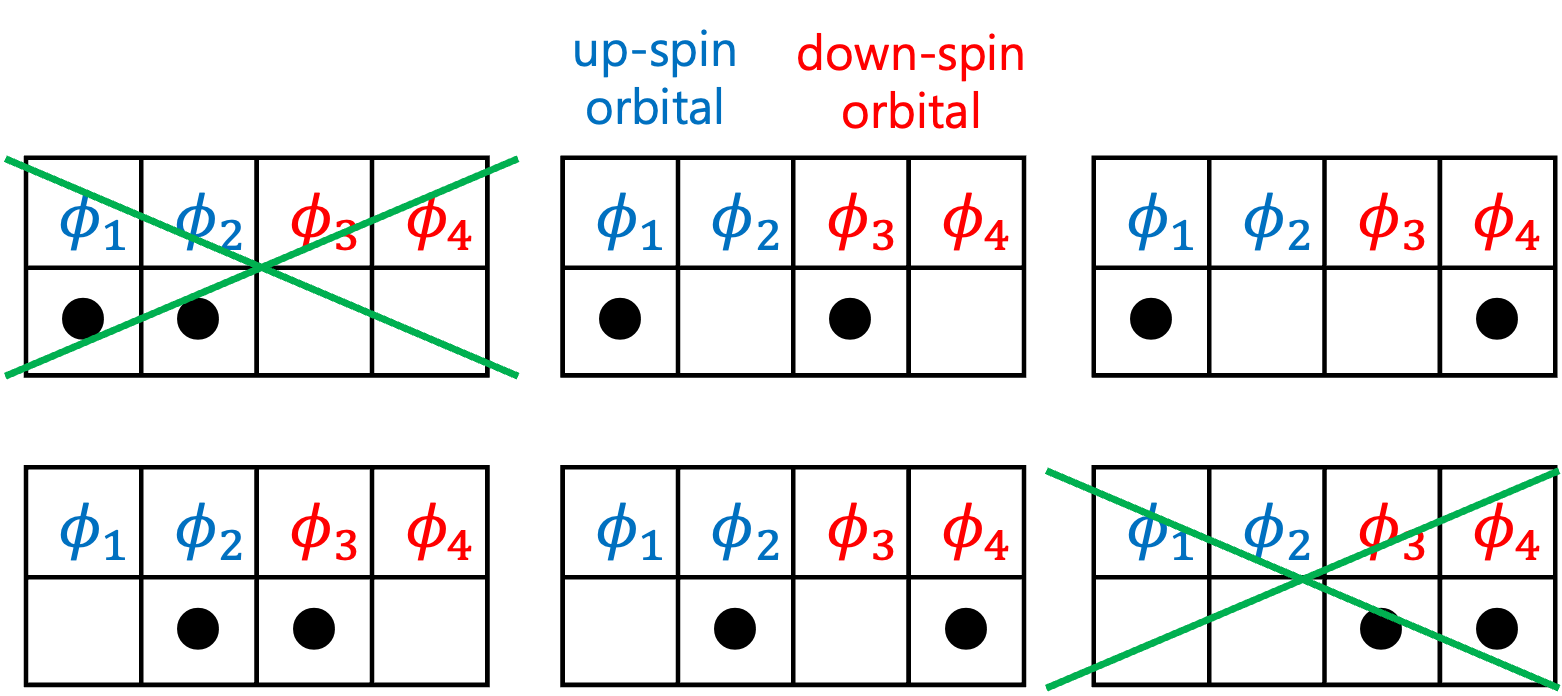
\includegraphics[width=0.45\textwidth]{fig/spin_cons.png}
  \caption{Validate Determinant of H2}
  \label{fig:example2}
\end{figure}

"전자의 수", "Multiplicity" 조건에 의해 유효한 Slater Determinant만을 추렸다. 따라서 H2의 파동함수는 해당 시스템에서 유효한 모든 Slater Determinant들을 basis로 표현될것이므로, 
파동함수를 아래와같이 기술 할 수 있다. 
\[
|\Psi_{FCI} \rangle = c_1|0101\rangle + c_2|0110\rangle + c_3|1001\rangle+ c_4|1010\rangle
\]

이렇게 기술해서 우리가 하고자 하는것은, 저 파동함수를 통해 \(\langle \Psi|\hat{H}|\Psi \rangle\)를 계산해서 가장 낮은 값을 구성하는 \(c_1, c_2, c_3, c_4 \) 를 찾으면 된다.
그리고 이러한 문제는 바로 고유값 문제를 통해 해결할 수 있다. 
그러기 위해 연산자꼴로 주어져있는 헤밀토니안 \(\hat{H}\) 를 저 4개의 basis로 구성된 공간에 사영시켜 헤밀토니안 행렬 \(\mathbf{H}\) 를 만들고, 
\begin{align*}
\mathbf{H}_{ab} &= \langle \Phi_a \vert \hat{H} \vert \Phi_b \rangle \\
\mathbf{H} &= \sum_a \sum_b \vert \Phi_a \rangle \langle \Phi_a \vert \hat{H} \vert \Phi_b \rangle \langle \Phi_b \vert
\end{align*}
그 행렬을 대각화하여 가장 낮은 값을 구성하는 \(c_1, c_2, c_3, c_4 \) 를 찾을 수 있고, 시스템이 가질 수 있는 가장 낮은 에너지(Ground-State Energy)를 계산할 수 있다. 
\[
\mathbf{H}\mathbf{c} = E\mathbf{c}
\]
이러한 계산방식을 FCI 방식 이라고 한다. 

\subsection{SCI(Selective Configuration Interaction)}
FCI 방식은 알려진 모든 계산방법중에 가장 정확한 계산을 수행한다. 하지만, 그 계산량이 매우 크다 \(H_2\) 시스템에 대해서 예시로써는 4개의 Slater Determinant 만을 사용했지만, 
일반적으로 스핀오비탈 M개, 전자 N개에 Singlet 인 시스템에 대해서 필요한 Slater Determinant의 개수는 아래와같다. 
\[
\text{number of Slater Determinant} = \binom{M/2}{N/2}\cdot\binom{M/2}{N/2}
\]

이것을 몇가지 시스템에 대해서 정리한것이 아래와 같다. 

\begin{figure}[htbp]
  \centering
  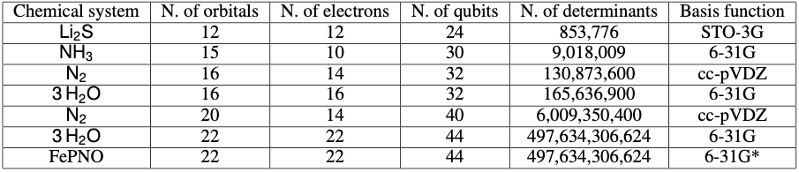
\includegraphics[width=0.8\textwidth]{fig/numofdet.png}
  \caption{number of Slater Determinant}
  \label{fig:example2}
\end{figure}
즉, 계산에 필요한 Slater Determinant 의 개수가 지수적으로 증가하게 된다. 따라서 이러한 방식은 실제 계산이 필요한 분자에는 적용할 수 없다. 그래서 제안된것이 SCI 방식이다.
이러한 계산들에서 계산량을 줄이기 위해서는 파동함수를 기술하는데에 필요한 Basis를 줄여야한다. 그러면서 동시에 비슷한 정밀도를 가져야한다. 
그래서 FCI 에서 파동함수를 기술했던 방식을 생각해보자. 
\[
|\Psi\rangle = \sum_I c_I |\Phi_I\rangle
\]
이는, 시스템의 조건들을 만족하는 모든 Slater Determinant를 basis로 사용한다. 분자에서의 임의의 양자상태를 표현하기에는 저렇게 해야만 할것이다. 
하지만, 우리의 계산에서 대부분의 목적은 바닥상태 에너지이다. 즉, 시스템이 가질 수 있는 가장 작은 에너지를 찾아보고자 하는 입장에서, 분명 그 바닥상태를 기술하는데에 기여가 적은 Slater Determinant가 있을것이다. 
그래서 그러한 상태들에 대해서는 무시하고, 정말로 바닥상태에 대해 기여가 큰 Slater Determinant만을 사용하여 파동함수를 표현하자는것이 바로 SCI 의 계산이다. 
\[
|\Psi\rangle = \sum_{I}^{D} c_I |\Phi_I\rangle \longrightarrow  |\Psi'\rangle = \sum_{I}^{D'} c'_I |\Phi_I\rangle 
\]
\[
\text{where,} \quad D' < D \left(= \text{number of Slater Determinant} = \binom{M/2}{N/2}\binom{M/2}{N/2}\right)
\]

Slater Determinant의 개수는 결국 파동함수를 나타내기 위한 basis의 개수이고, basis가 정의되므로, 그 basis로 구성되는 공간들을 생각해볼 수 있으며, SCI 에서 찾고자 하는것은, 아래의 모식도에서의 Core Space 이다. 

\begin{figure}[htbp]
  \centering
  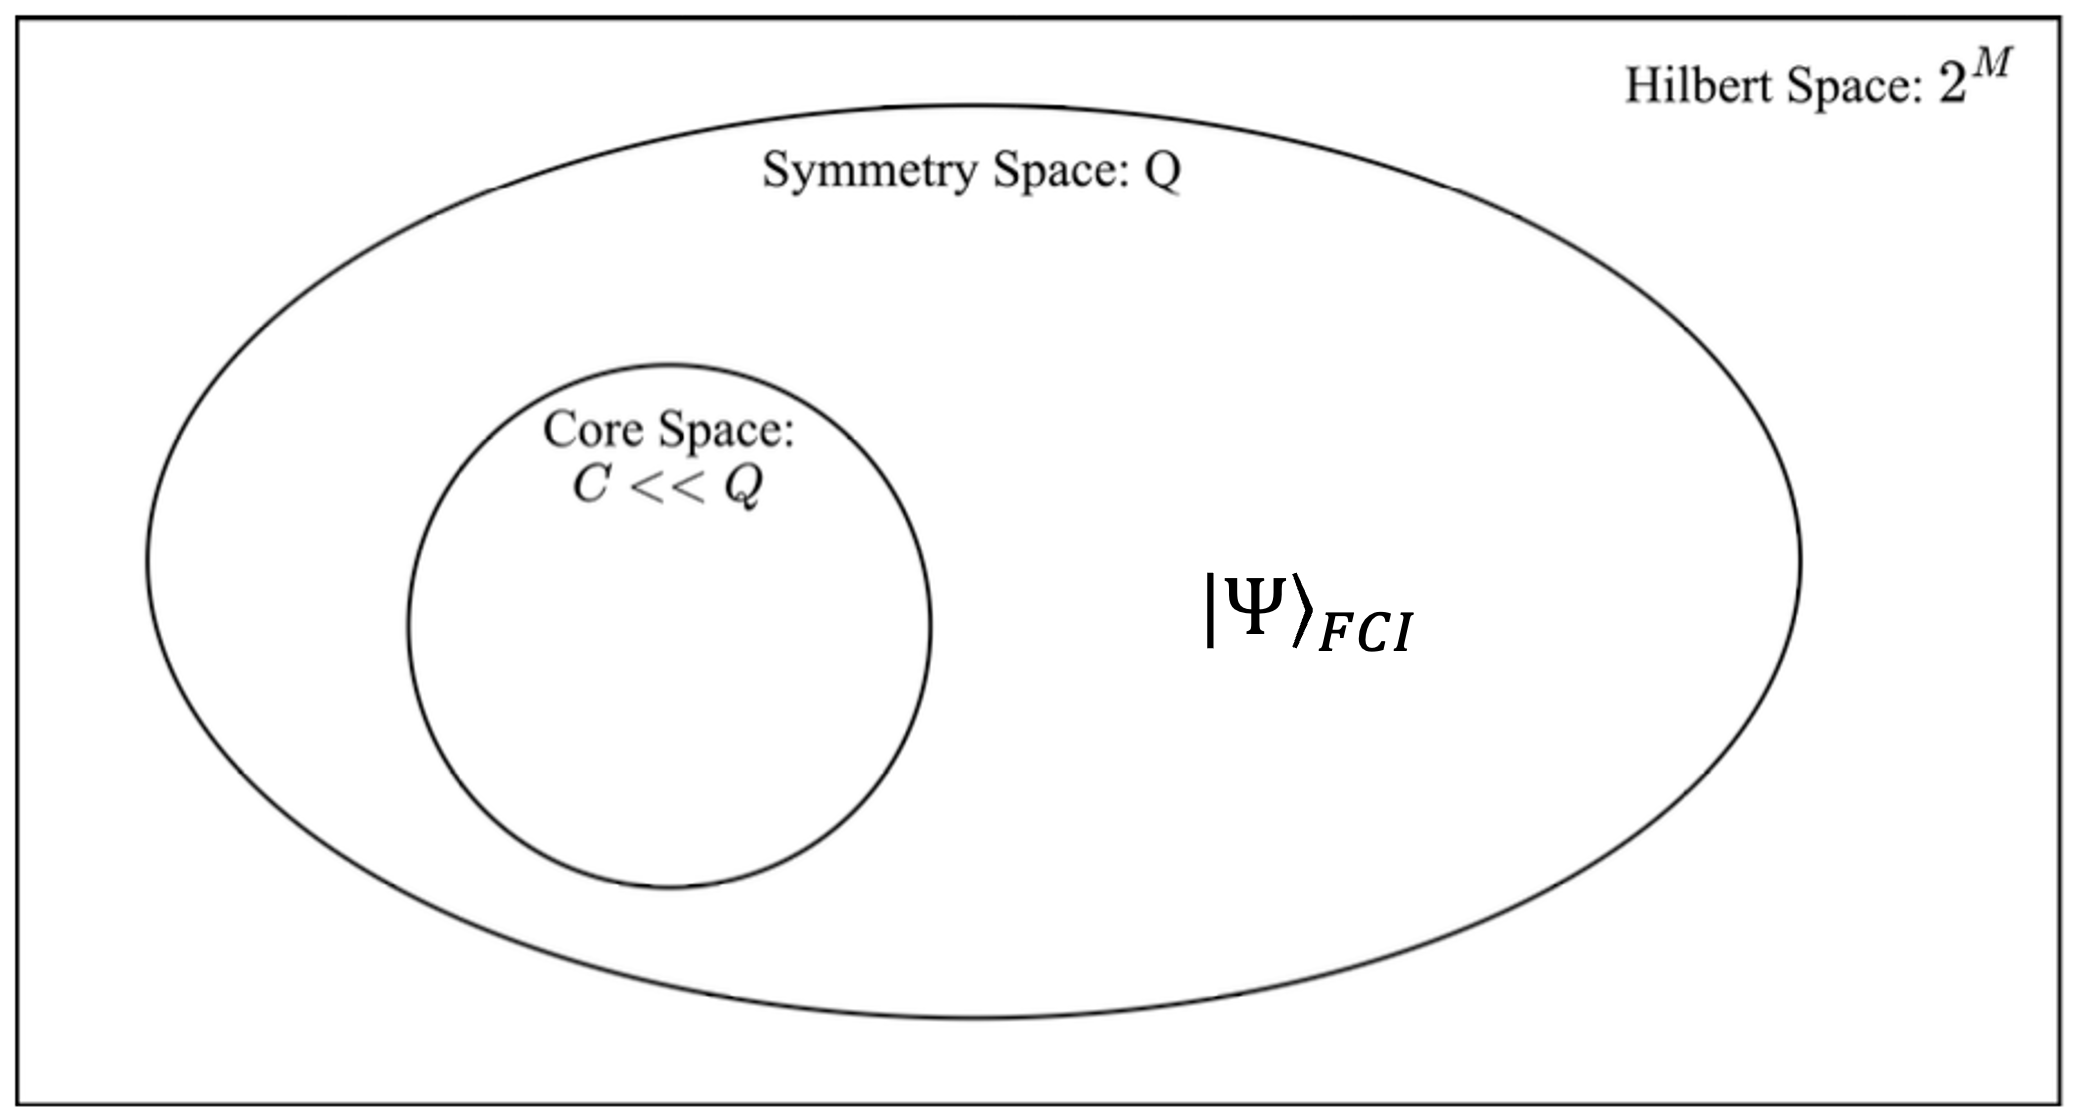
\includegraphics[width=0.6\textwidth]{fig/space.png}
  \caption{Relation of Space}
  \label{fig:example2}
\end{figure}

M개의 스핀오비탈을 갖고있는 시스템에 대해서 구성할 수 있는 Slater Determinant 의 개수는 \(2^M\) 개 이고, 이러한 모든 Slater Determinant를 basis로 하여 구성되는 공간을 Hilbert Space 라고 정의해보자. 
하지만, 여기에 시스템이 갖는 전자수 보존, Multiplicity 조건, 등을 이용하면, 물리적으로 맞지 않는 Slater Determinant를 제외하여, \(\binom{M/2}{N/2}\binom{M/2}{N/2}\)개 만을 basis로 사용하여 파동함수를 
표현 할 수 있게된다. 즉 기존의 Hilbert Space의 부분공간 Symmetry Space를 정의할 수 있게되며, 이 공간은 시스템을 효율적으로 표현할 수 있는 공간을 의미한다.
이렇게 Hilbert Space중에서도 유의미한 Basis만을 택하여 symmetry Space를 정의한 것 처럼, symmetry Space안에서도 그중에서 바닥상태를 더 잘 기술할 수 있는 basis들로 구성된 Core Space가 있을것이라는 
기대로 여러 방법을 통해 Core Space를 찾고자 하는 방식이 SCI 이다. 하지만, 어떤 basis(Slater Determinant)가 기여가 클지, 작을지를 판단하는것이 간단한 일은 아니다.
따라서 여기에다가 양자컴퓨터를 사용해보자 라는 아이디어를 이용해서, FCI 에서의 Hilbert Space 보다 더 작은 부분공간을 구성해보자 하는시도가 바로 이어서 설명할 QSCI 계산방법이다. 


\subsection{QSCI(Quantum Selected Configuration Interaction)}
이부분에서 어쩔수없이 계속 들고오고 있는데, 분자의 파동함수는 결국 아래와같이 기술될것이다. 
\[
|\Psi\rangle = \sum_I c_I |\Phi_I\rangle
\]
이제 여기서부터는 양자컴퓨팅과 관련된 이야기가 들어가기 시작한다. 결국 \(|\Phi_I\rangle\) 는 한 Slater Determinant이자, binary String 으로 표현된다. 
그리고 이러한 양자상태를 양자컴퓨터에서 계산을 하기위해 양자 회로로 구현하게 되는데, 이때 저 binary String 을 그대로 큐비트의 0과 1상태로 매핑할 수 있다.(Jordan-Wigner Mapping)
이제 그럼 예를 들어 아래와같이 표현할 수 있는데, 이게 둘다 0,1로 표현되고 Braket Notation을 사용하고 있어 표현되는 방식이 같다. 
\begin{align*}
|\Phi\rangle  &= \vert 10011010 \rangle \quad \text{(Occupation number Representation of Slater Determinant)} \\
|\Phi\rangle  &= \vert 10011010 \rangle = \vert 1 \rangle \otimes \vert 0 \rangle \otimes \cdots \otimes \vert 0 \rangle \quad \text{(Qubit States corresponded to Slater Determinant)}
\end{align*}
그런데 이렇게하면 이제 저 파동함수의 표현에 있어서 하나의 Slater Determinant \(|\Phi_I\rangle\) 에 대한 선형계수 \(c_I\) 를 
하나의 큐비트상태 \(|\Phi_I\rangle\)에 대한 선형계수로써 해석할 수 있게되고, 이는 확률로써 해석 할 수 있게된다. 
\begin{figure}[htbp]
  \centering
  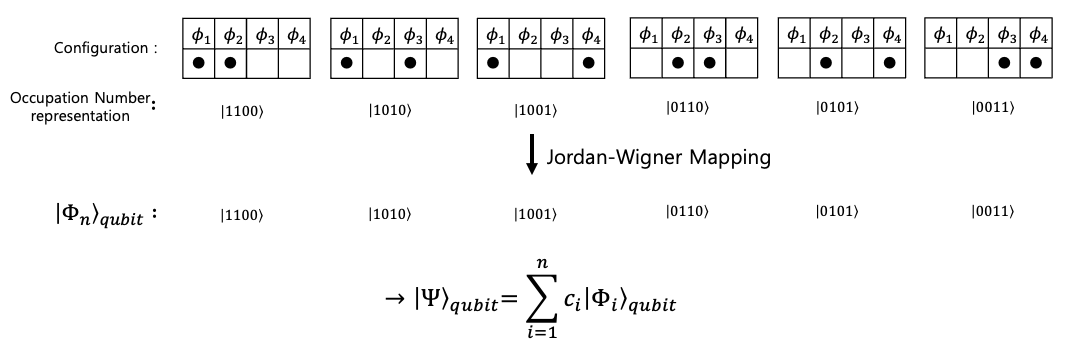
\includegraphics[width=0.9\textwidth]{fig/QSCI3.png}
  \label{fig:example2}
\end{figure}

즉, 어떤 다른 알고리즘들을 이용하여 바닥상태에 대응되는 파동함수를 양자 회로로써 얼추 비슷하게만 표현 해두면, 그 회로를 여러번 측정하여, 각 스트링들에 대한 확률을 얻을 수 있고, 
그 확률을 통해 각 Slater Determinant(양자 회로에서는 Qubit State)에 대응되는 선형 계수를 구할 수 있게된다. 
그리고 그 선형 계수를 사전에 지정할 수 있는 \(\epsilon\) 이라는 값과 비교하여 이보다 작을경우, 그 basis를 무시하여 더 적은 basis로 효율적으로 상태를 표현할 수있는 Core Space 를 구성 할 수 있고, 
\[
|\Psi_{QSCI}\rangle = \sum_{I=1}^{n'} c_I |\Phi_I\rangle 
\]
\[
\text{where,} \qquad n'<<n, \qquad c_i \geq \epsilon
\]
더 작은 차원에서 헤밀토니안 행렬을 구성하여 
\begin{align*}
\mathbf{H} = \sum_{a,b=1}^{n'} \vert \Phi_a \rangle \langle \Phi_a \vert \hat{H} \vert \Phi_b \rangle \langle \Phi_b \vert
\end{align*}
대각화 문제를 통해 문제를 해결 할 수 있다. 이렇게 계산을 하는방식이 바로 QSCI 이다. 하지만, 이또한 한가지 문제점이 있는데, 
저 \enquote{얼추 비슷한 상태} 를 어떻게 만들것인가 이다. 결국 VQE 쓸건지, 아니면 다른 획기적인 방식이 있는가에 대해서는 여전히 잘 모르는 부분이다. 
그래서 이러한 문제점을 보완하기 위해 이제 드디어 이 논문에서 제안한 방식을 다룰것이다. 

\section{HIVQE}
이제부터 HIVQE 와 관련된 내용을 다뤄볼것이다. 사실, 사전지식이 많이 필요했을뿐, 알고리즘자체로 다뤄야할 내용은 많지않다. 일단 지금까지 언급했던 두개의 양자화학계산 양자컴퓨터알고리즘인 VQE 와 QSCI의 간단한 pipeline을 살펴보자. 
\begin{figure}[H]
  \centering
  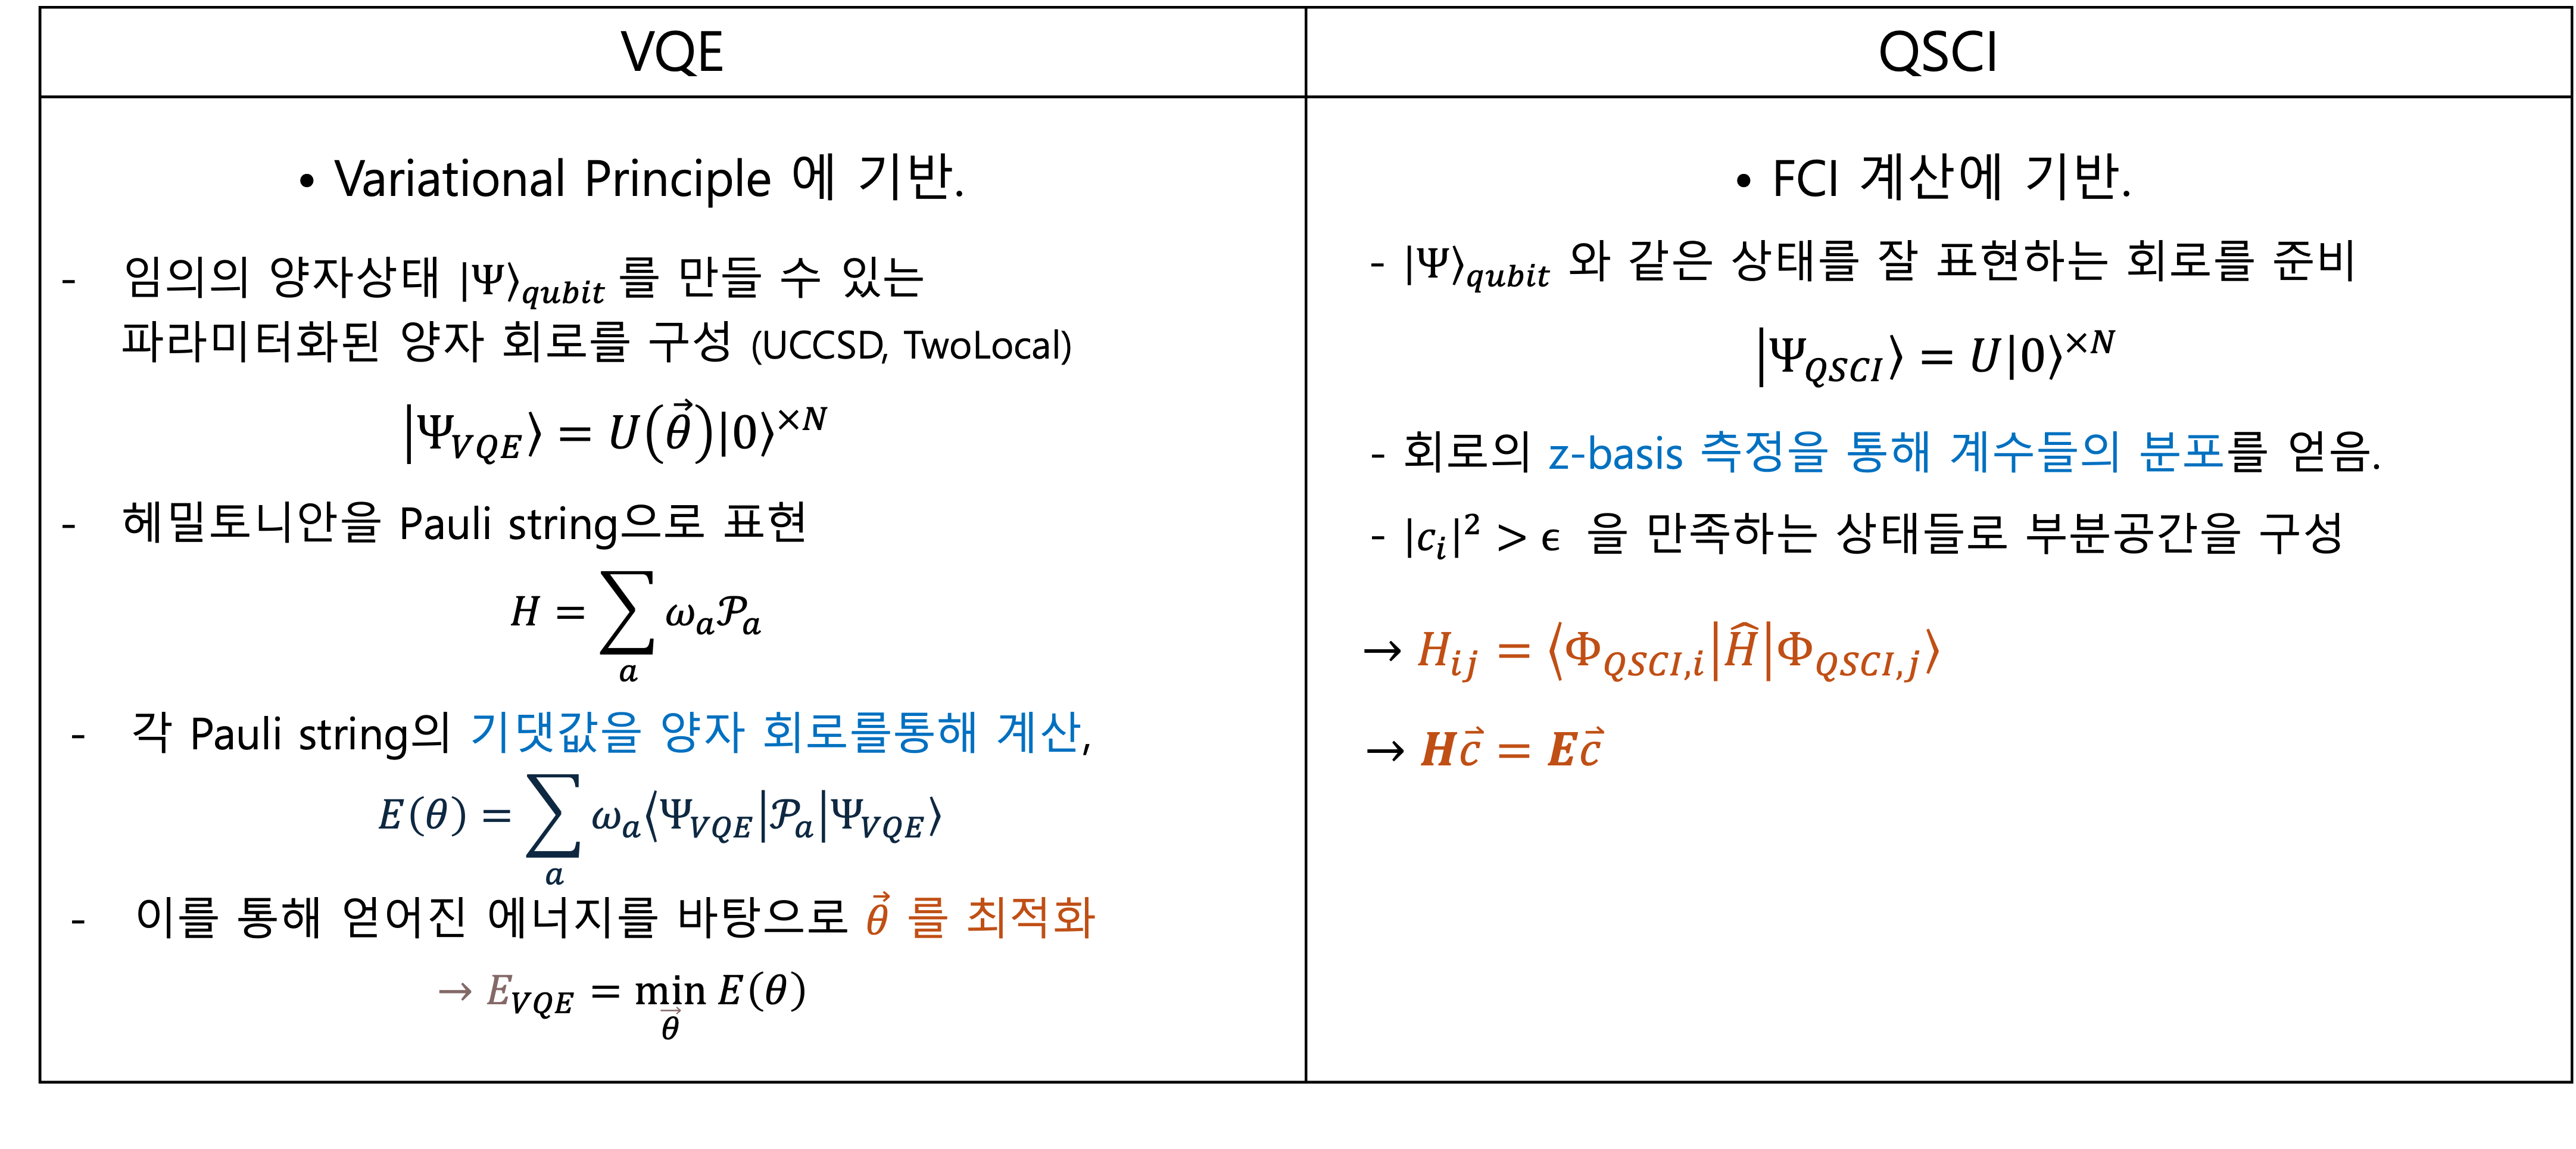
\includegraphics[width=\textwidth]{fig/VQE,QSCI2.png}
  \label{fig:example2}
\end{figure}
VQE 에서는 양자회로를 파라미터를 이용해 구성하여 매 Iteration 에서 헤밀토니안에 대한 기댓값을 측정하고 그 기댓값을 바탕으로 회로의 파라미터를 최적화하는 방식으로 진행된다. 

하지만, 이는 구성된 모든 파울리 스트링에 대해 회로를 측정해야하고,(즉, 총 shot수 = 파울리스트링의 개수\(\times\)shot수 )
파라미터를 통해 구성한 양자상태, 즉 각 Slater Determinant의 선형계수가 직접적으로 에너지의 정밀도에 영향을 주게되어, 소위 Barren Plateau 의 문제에 빠지기 쉽고, 실제로 시스템이 커질수록 에너지 계산이 어려워진다. 
QSCI 알고리즘은 양자상태의 선형계수가 에너지 계산에 사용되기는 하지만, 직접연관되진 않고, 단순히 선형 계수가 특정 임계값보다 큰 모든 상태를 사용하여 고전적으로 계산을 수행하기때문에, 
상태가 비교적 잘 구성되어있다면, 그 상태가 아주정확하지 않더라도 에너지를 정확하게 계산할 수 있다. 하지만, 그 상태를 잘 만드는것이 쉽지않다. 
그래서 이 두가지 장점을 적절히 섞어보자는것이다.
\begin{figure}[H]
  \centering
  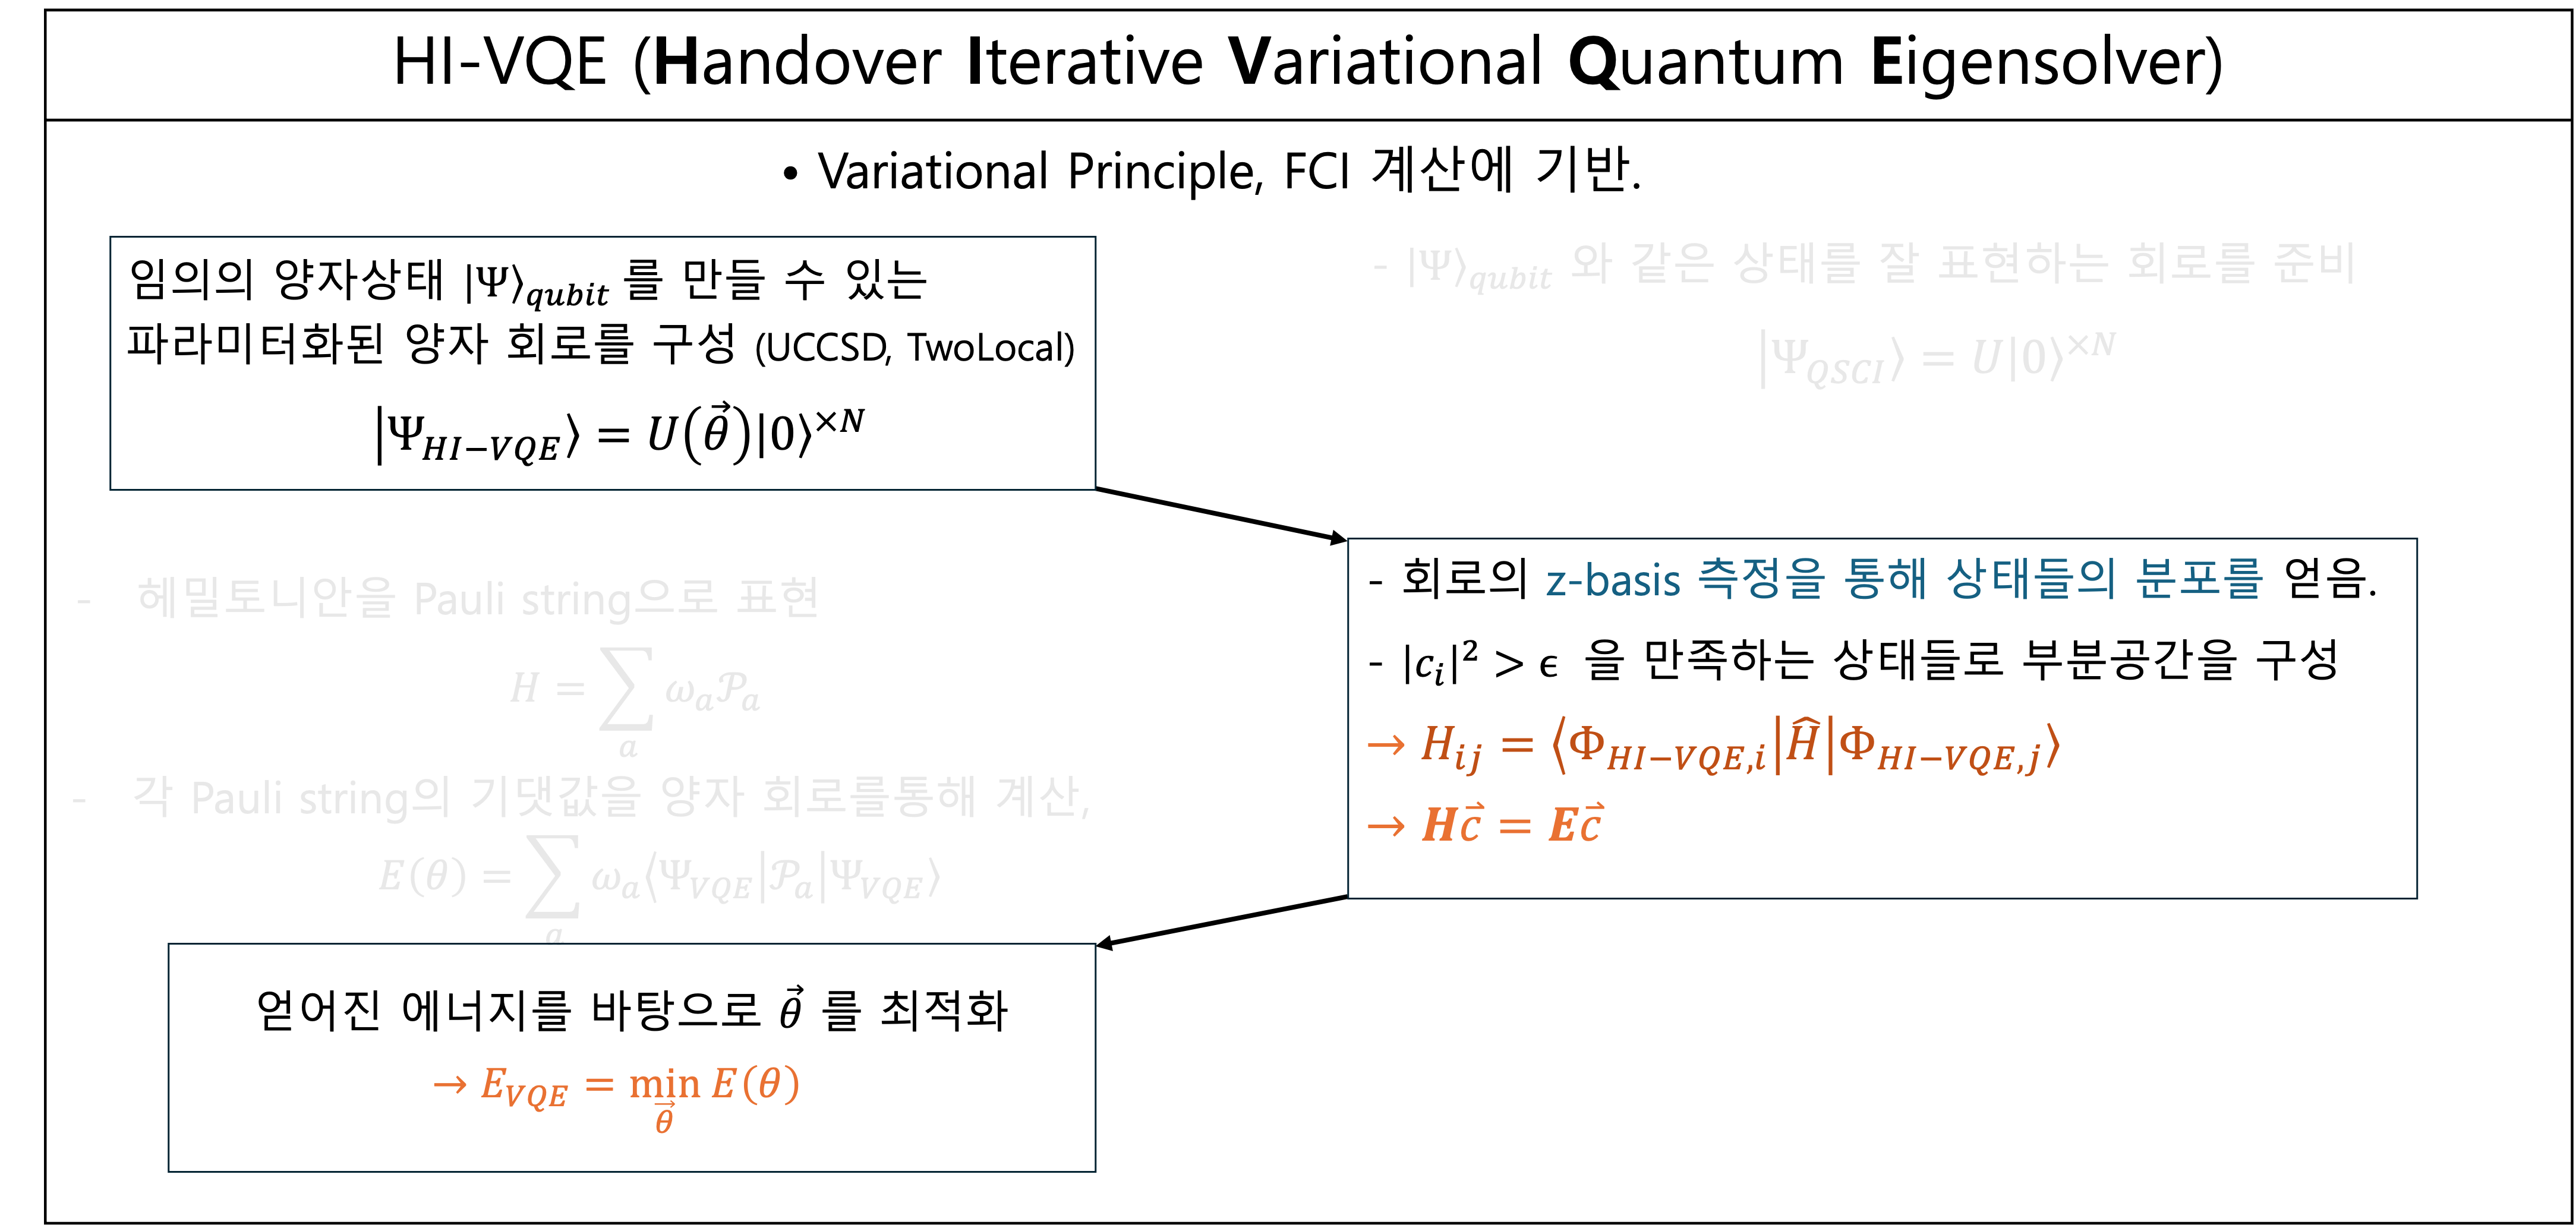
\includegraphics[width=\textwidth]{fig/HIVQE_table.png}
  \label{fig:example2}
\end{figure}
VQE 알고리즘은 최적화 과정을 이용할 수 있다는 장점이 있었지만, 계산이 오래걸리고 상태의 선형계수등이 정밀도에 직접적으로 영향을 준다는 제한점이 있었고, 
HIVQE는 아주정확한 양자회로를 만들 필요는 없지만 적절한 상태를 만드는게 어려웠으니, 
이를 적절히 조합해서, 최적화 할 수 있는 양자회로를 구성하고, 각 Iteration 에서는 QSCI 알고리즘과 유사한 방식으로 에너지를 계산하고, 이를 최적화 하자는것이 HIVQE 이다. 
이렇게하면, 최적화과정으로 Ground-State Energy를 잘 찾아갈 수 있으며, 그 최적화 과정이 아주 정확하지 않더라도, 에너지의 계산방법이 그 선형계수등에 직접적으로 영향을 받지 않기때문에
효과적으로 정밀도를 확보할 수 있다. 이제 이 과정을 디테일하게 이어가보자. 

\subsection{Method}
이게 과정이 여러 스텝이 있는데, 이를 천천히 따라가보자. 
\begin{figure}[htbp]
  \centering
  \begin{subfigure}[b]{0.45\textwidth}
    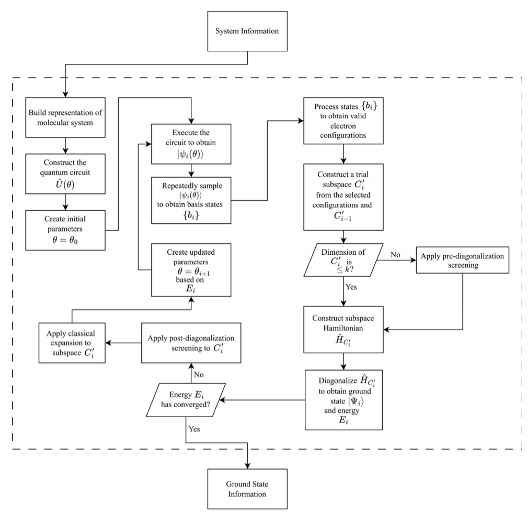
\includegraphics[width=\textwidth]{fig/HIVQE_paper.png}
    \caption{논문의 모식도}
    \label{fig:first}
  \end{subfigure}
  \hfill
  \vrule width 1pt  % 수직선 추가 (굵기: 1pt)
  \hfill
  \begin{subfigure}[b]{0.45\textwidth}
    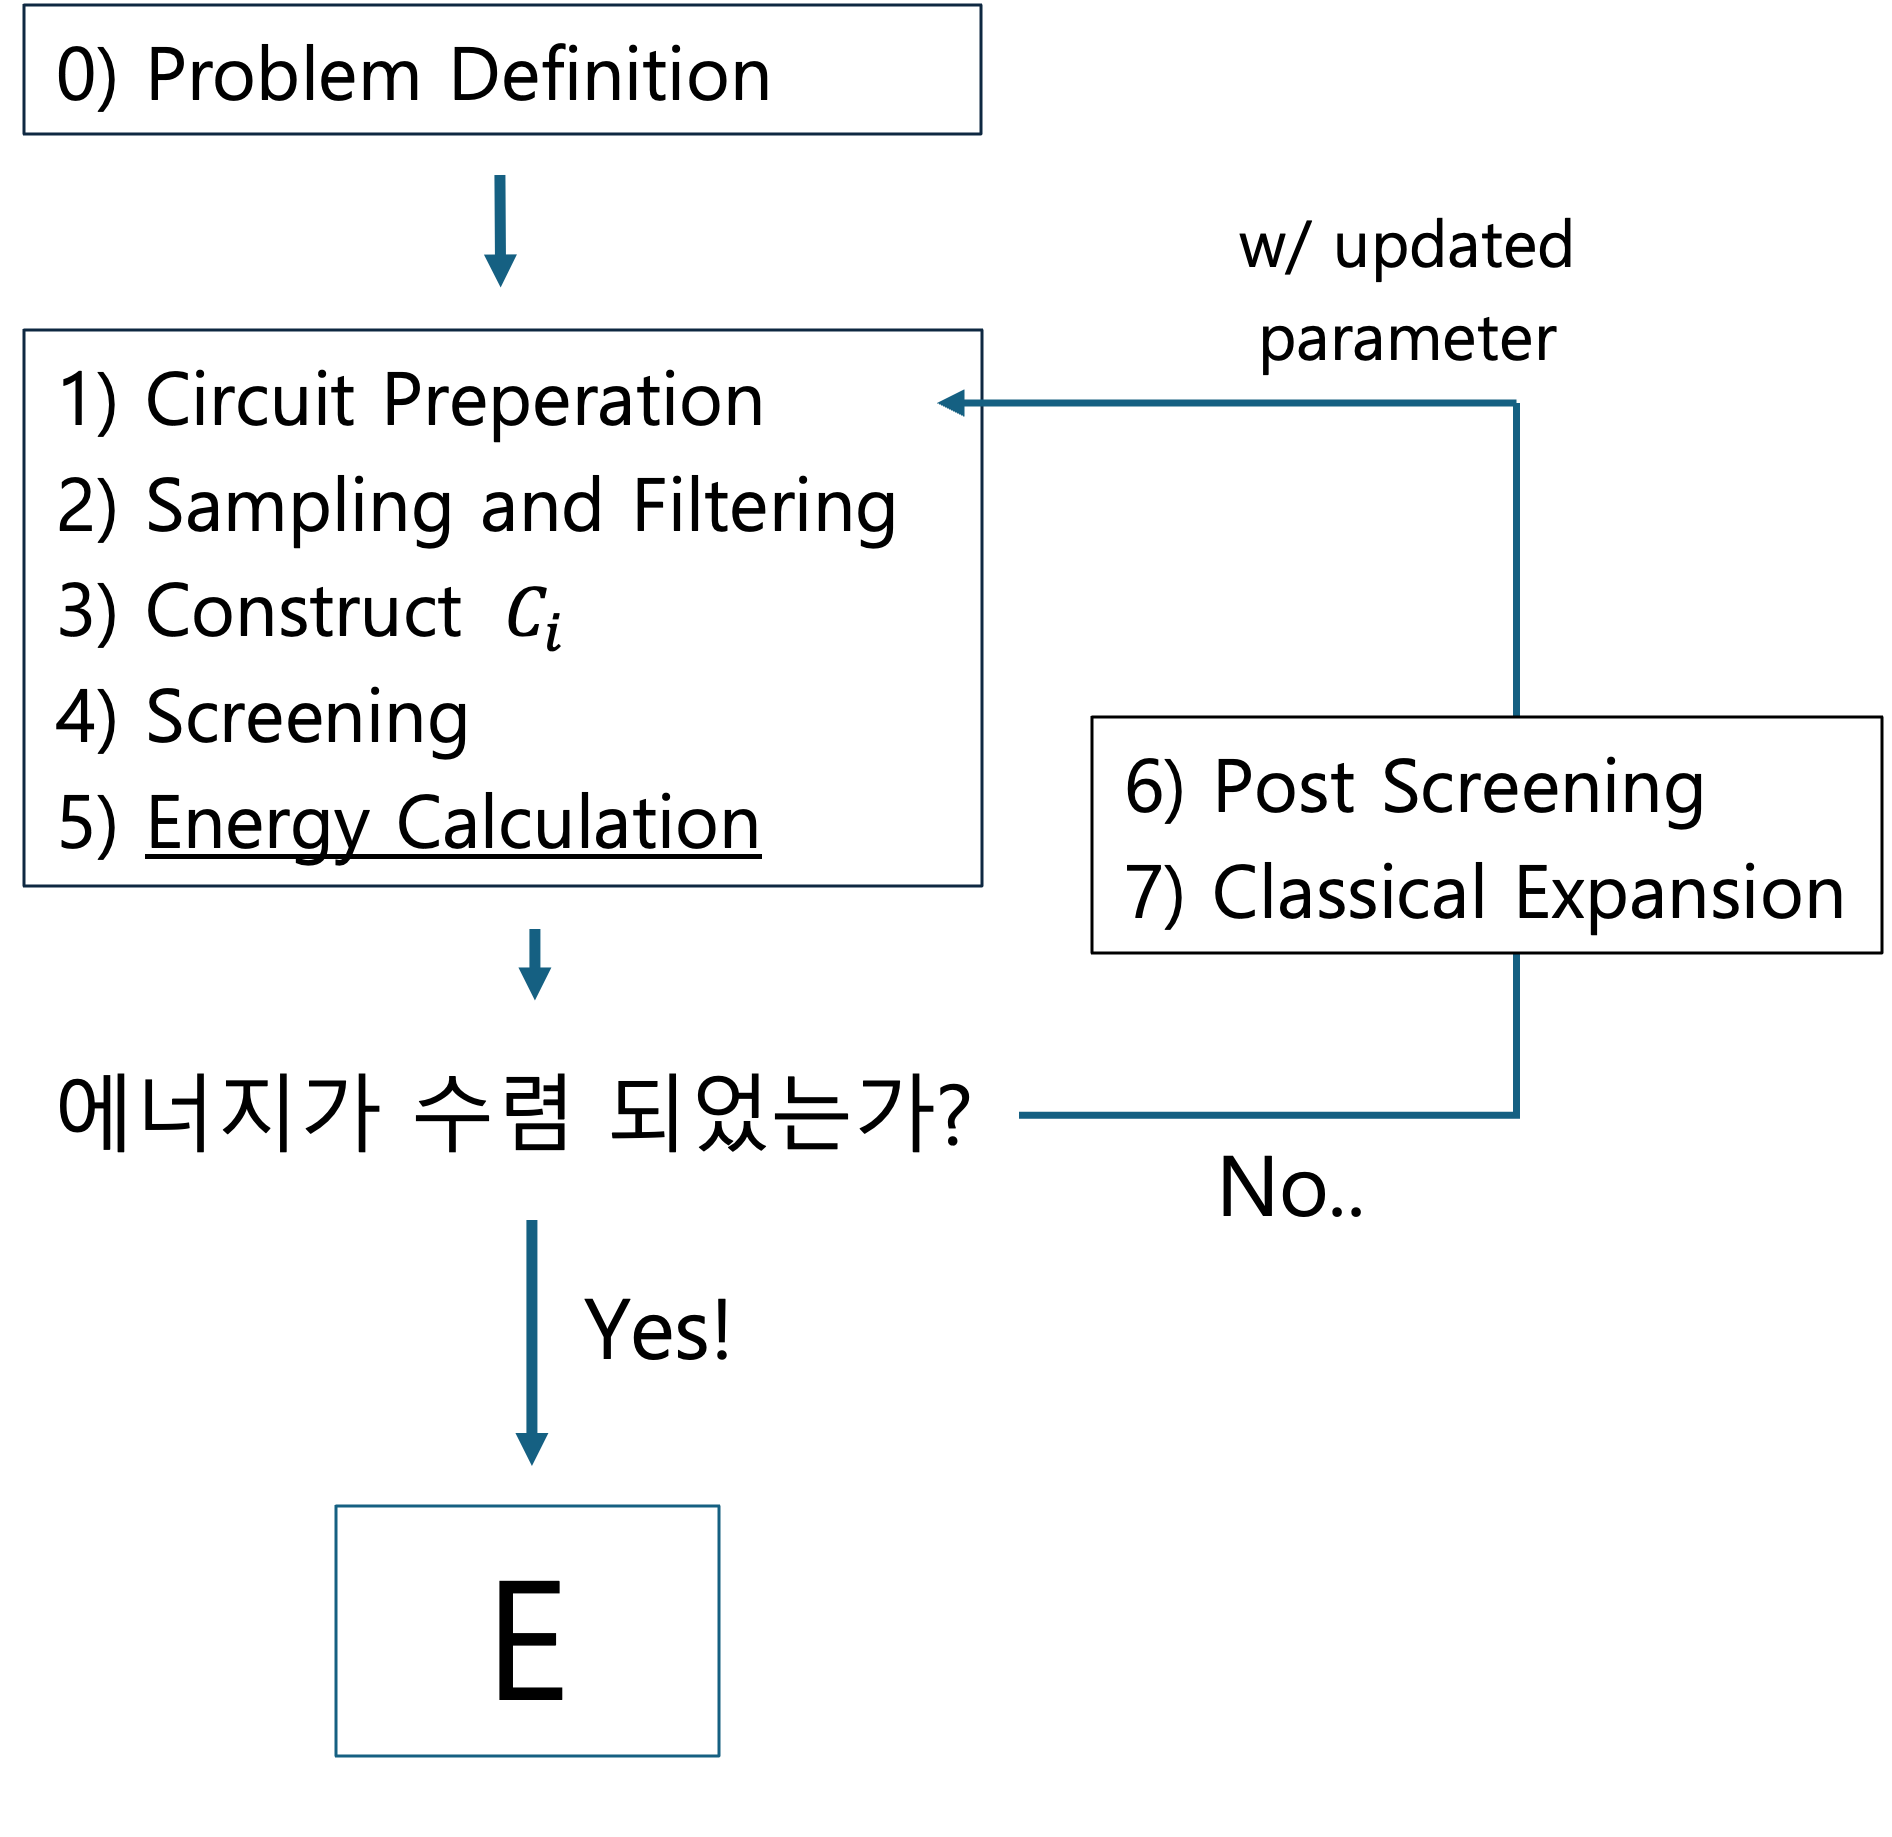
\includegraphics[width=\textwidth]{fig/HIVQE_my.png}
    \caption{내가정리}
    \label{fig:second}
  \end{subfigure}
  \caption{HIVQE pipeline}
  \label{fig:two_figures_side_by_side}
\end{figure}
왼쪽이 논문에서 제시한 모식도 이고, 오른쪽이 내가 정리한 그림이다. 
왼쪽에서 하는 계산들이 오른쪽의 목차에도 다 반영이 되어있으니, 오른쪽그림을 기준으로 설명을 이어가보자. 
여기서부터는 이제 Practical 한 내용들을 다루면서 내용과 함께 어떻게 구현하는지도 같이 이야기를 가보자. 

\subsubsection{Problem Definition}
여기는 이제 사실 이론적인 내용은 없다. 
하는 이유는 우리가 바닥상태 에너지를 계산하고자 하는 어떤 분자가 있을텐데, 그 분자의 에너지를 계산하려면, 
그 분자에 해당하는 헤밀토니안이나, 어떤 전자의 개수, 오비탈의 개수와같은 정보들이 필요할텐데, 이를 만들어주는 패키지를 이용하게된다. 
Molecularinfo 에 시스템을 구성하는 각 원자들의 종류와 위치, 그리고 총 시스템의 전하량과 Multiplicity까지 총 4개? 의 정보를 넣어주게되면,
그 시스템에 맞는 헤밀토니안과 각 정보들을 담은 하나의 클래스를 만들어준다. 이후의 계산들은 이 클래스에서 정보를 가져와서 계산을 진행하게 된다. 
그래서 코드의 초반에는 이러한 코드가 들어가게 된다. 

\subsubsection{Circuit Preperation}
결론적으로 HIVQE 에서 해야하는것은, 각 Slater Determinant중 바닥상태에 기여가 높은 상태를 찾아내는것이다. 
기여가 높다는것은 바닥상태를 표현할때 각 Slater Determinant의 선형계수가 가장 높은것들을 찾으면 된다. 
그러기 위해 HIVQE 에서는 양자 회로의 샘플링을 통해 이러한 과정을 진행할것이고, 따라서 적절한 양자회로를 구성해야한다. 
하지만 QSCI 에서처럼 어떤 그럴듯한 회로가 있는것이 아니므로, 파라미터화된 양자회로를 구성하는것이 필요하다. 
이 파라미터화된 양자회로, PQC(Parameterized Quantum Circuit) 라고하는것은 구성하는데에 있어서 두가지의 척도가 있다. 
첫째는 얼마나 파라미터를 이용해 주어진 Hilbert Space에서의 임의의 상태를 얼마나 잘 표현하는가 에 해당하는 표현력이고
둘재는 얼마나 파라미터의 최적화를 통해 주어진 상태를 잘 찾아가는가에 대응되는 학습력이 있다. 
이 표현력과 학습력은 보통 Trade-off 관계에 있으며, 문제에 적절한 회로를 선택하는것이 중요하다. 
이러한 파라미터화된 양자회로를 소위 Ansatz 라고 부르며, 이 Ansatz를 만드는 방법에는 크게  1)Problem-inspired 방식과 2)Hardware-Efficient 의 두가지 방법이 있다. 
각 방식을 간단하게 살펴보자. 

\begin{enumerate}[label=\(1\))]
\item {Hardware-Efficient Ansatz}
\begin{figure}[H]
  \centering
  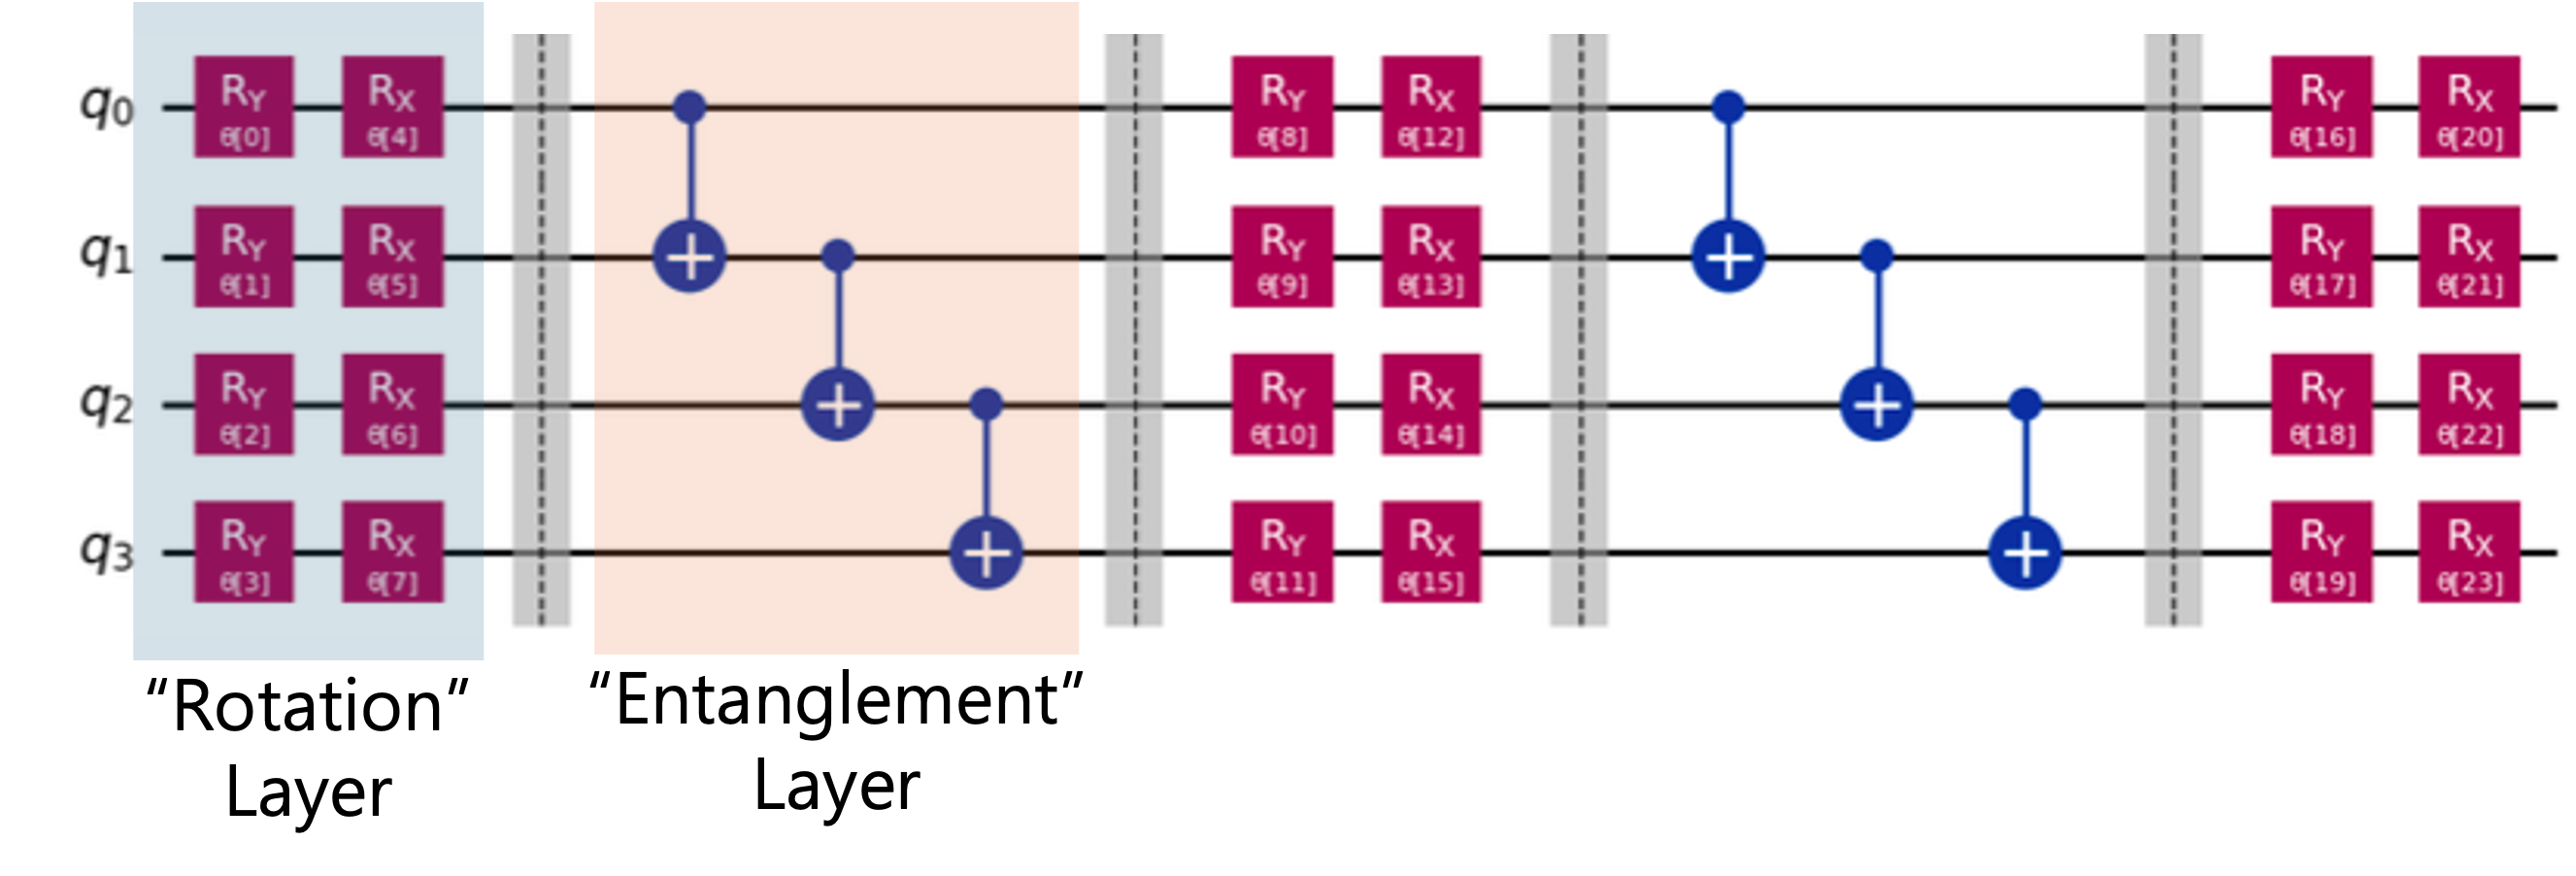
\includegraphics[width=0.8\textwidth]{fig/twolocal.png}
  \caption{twolocal Circuit}
  \label{fig:example3}
\end{figure}
첫번째 방식은 Hardware-Efficient 한 Ansatz의 예로 Twolocal Ansatz를 다뤄볼것이다. 
Hardware-Efficient 한 Ansatz 라는것은 말그대로 풀고자하는 문제와 상관없이, 큐비트의 공간에서 임의의 상태를 만들어보자 라고하는것이다. 
여기서, Twolocal Ansatz 경우 임의의 single qubit의 양자상태는 두개의 Rotation Gate를 통해 만들 수 있다는점에 착안하여, 
두개의 Rotation Gate로 이루어진 Rotation Layer 와 Multi qubits 시스템이 갖는 특징인 Entanglement 를 CNOT 게이트로 구성된 Entanglement Layer를 번갈아여 구성한다. 
여기서  Rotation Gate의 각도를 파라미터로하여 임의의 양자상태를 표현하게 된다. 하는 Ansatz이다. 이러한 Ansatz를 twolocal 혹은 Efficient SU2 라고 한다. 
\end{enumerate}

\begin{enumerate}[label=\(2\))]
\item {Problem-inspired Ansatz}
두번째는 Problem-inspired Ansatz 의 한 예시로 UCCSD 방법을 살펴보자.
Problem-inspired Ansatz 라는것은 이번에는 풀고자하는 문제에 대해 임의의 양자상태를 구성하고 이를 양자 회로로 인코딩하는 방법이다. 
그중 UCCSD(Unitary Coupled Cluster Singles and Doubles) Ansatz의 경우 기존의 양자화학계산인 CCSD 에서의 계산방법에 착안하여
분자가 가질 수 있는 여러 Configuration들에 대응되는 Slater Determinant 를 basis로 양자상태를 표현한다. 
이때 각 Configuration은 어떤 기준상태(Hartree-Fock State)의 Excitation으로 기술 될 수 있으며, 따라서 각 Configuration은 생성/소멸 연산자로 표현될 수 있다. 
\[
\ket{\Psi_{\mathrm{UCCSD}}}
   \;=\;
   \exp\bigl(\hat{T} - \hat{T}^\dagger\bigr)\,\ket{\Phi_0},
\]
\[
\hat{T} \;=\; \hat{T}_1 + \hat{T}_2,
\]
\[
\hat{T}_1 \;=\; \sum_{i,a} t_i^a \,a_a^\dagger\,a_i,
\qquad
\hat{T}_2 \;=\; \frac{1}{4}\sum_{i,j,a,b} t_{ij}^{ab}\;a_a^\dagger\,a_b^\dagger\,a_j\,a_i.
\]

\begin{itemize}
  \item \(i,j\): 점유 궤도(occupied orbitals)
  \item \(a,b\): 미점유 궤도(virtual orbitals)
  \item \(t_i^a,\,t_{ij}^{ab}\): 클러스터 진폭(cluster amplitudes)
\end{itemize}
이렇게 문제에 맞는 헤밀토니안을 구성하고, 이를 파울리 게이트로써 Mapping 하게되면, 헤밀토니안에 잘 맞는 Ansatz를 구성할 수있으며, 이러한 형태의 Ansatz를 UCCSD Ansatz라고 한다. 
\end{enumerate}

적어도 VQE의 맥락에서는 UCCSD의 Ansatz가 표현력및 학습력의 부분에서 더 좋은 성능을 보이는것이 일반적이다. 하지만, HIVQE 에서는 상태의 "표현력" 자체가 계산의 에너지의 정밀도에는 크게 영향을 미치지 않는다. 
그리고, 기본적으로 이 알고리즘의 최종목표는 아주 큰 시스템의 에너지를 계산하는것인데, UCCSD Ansatz의 경우 회로의 Cost가 매우 크다. 
따라서 HIVQE 에서는 twolocal Ansatz를 이용하여 실험중에 있다. 

\subsubsection{Sampling and Filtering}
헤밀토니안을 projection 할 Slater Determinant를 basis로 하는공간을 구성하기 위해 
이제 주어진 양자회로로 부터 Slater Determinant들을 Sampling 할것이다. 
양자회로를 z-basis 측정 함으로써 각각의 큐비트의 상태에따라 0과 1의 binary string을 얻게된다. 
그리고 각 binary 스트링은 Slater Determinant에 대응된다. 
따라서 양자회로를 원하는 Sampling 횟수만큼 작동시켜 그 갯수만큼의 Slater Determinant를 얻고, 그 얻어진 공간을 core space로써 사용할것이다. 
하지만, 이때 Slater Determinant가 만족해야할 두가지의 조건이 있다고 위에서 이야기 했었다.
첫째는 전자수의 보존이고, 둘째는 Multiplicity의 보존이다.
이 두가지의 조건을 만족하지 않는 Slater Determinant는 버린다(Filtering)
전자수의 보존을 만족시키기위해 Sampling 된 binary String 에서 1의 합이 시스템의 전자수 N 과 같지 않은 상태는 모두 버린다. 
또 Multiplicity의 보존을 위해, binary String 의 앞의 절반(up-spin orbital)에서의 1의 개수와 뒤의 절반(down-spin orbital)에서의 1의 개수의 차이를 \(\Delta S\) 를 확인하면,
시스템의 스핀 각 운동량은 \(\frac{1}{2}\Delta S\) 가 되고, 따라서 Multiplicity는 \(\Delta S + 1\) 이 된다. 
이때 이 \(\Delta S + 1\) 가 원하는 Multiplicity 가 아닌경우(ex, in singlet, Multiplicity=1)그 String을 버린다. 
이 두가지 조건을 모두 만족하는 String(Slater Determinant)만을 모아 Filtered Basis집합 \(\{b'_i\}\)를 구성한다. 

\subsubsection{Construct \(C_i\)}
이전 과정에서 Sampling 된 상태에 Filtering을 하여 만들어진 Filtered Basis 를 이용하여 i번째 Iteration 에서 사용할 Core Space \(C_i\)를 구성한다. 
\[
C'_i = \text{span}\{b'_i\}
\]
prime 을 붙힌 이유는 이것만을 사용하는것이 아니라, 이전 Iteration 에서 사용된 공간인 \(C_{i-1}\)에 약간의 가공을 하여(Post Screening, Classical Expansion 과정, 이후 설명) \(\tilde{C}_{i-1}\) 공간을 합집합 하여
i번째 Iteration 에서 사용할 Core Space \(C_i\)를 구성하게 된다. 
\[
C_i = C'_i \cup \tilde{C}_{i-1}
\]
\subsubsection{Screening}
제약없이 매 Iteration에서 \(C_i\) 를 구성하게되면, 각 차원이 계속 커지게 된다. 이는 계산 Cost의 증가를 의미하고 이는 우리가 원하는 바가 아니므로, 그 기여가 적은 basis(Slater Determinant)를 버린다. 이 과정을 Screening이라고 한다. 
그래서 기본적으로 이 과정은 \(C_i\)의 차원\(\left(D_{i}\right)\)이 사전에 지정된 특정 값 \(k\) 보다 클 경우에 수행한다. 
\begin{enumerate}[label=\(\ast\)]
\item {참고}

이 k값은 논문에서 계산한것은 \(2 \times 10^{4} \thicksim  2 \times 10^{6}\) 정도의 스케일이다. 일단 내가 실험으로 구현중인 계산에서는 k= 2000정도로 하여 실험중에 있다. 
\end{enumerate}
그래서 할것은 \(C_i\) 공간에 헤밀토니안을 사영(projection) 시키는것이다. 
\(C_i\) 공간의 basis sets인 \(\{b_i\}\)는 아래와같을 것이다. 
\[
\{b_i\} = \{\vert \Phi_1 \rangle, \vert \Phi_2 \rangle, \cdots, \vert \Phi_{D_i} \rangle \}
\]
따라서 \(C_i\)로의 사영은 아래와같이 정의된다. 
\[
\mathbf{H} = \sum_{a,b=1}^{D_i} \vert \Phi_a \rangle \langle \Phi_a \vert \hat{H} \vert \Phi_b \rangle \langle \Phi_b \vert
\]
따라서 \(\mathbf{H}\) 는 \(D_i \times D_i \) 차원의 행렬이 된다. 
여기서 \(\langle \Phi_a \vert \hat{H} \vert \Phi_b \rangle\)의 계산은 3.1.6 Energy Calculation 에서도 쓰이는 계산이며,
HIVQE에서 가장 긴 소요시간이 걸리는 과정이다. 

이 계산과정에 대한 디테일은 3.1.6 Energy Calculation 이후에 한꺼번에 다루겠다. 일단은 저런 계산을 한다 라는것만 이해하자. 

이제 \(C_i\) 공간에 사영된 헤밀토니안 을 대각화 한다. 즉, 헤밀토니안의 고유상태를 \(\{b_i\}\) 들의 선형결합으로 나타내자는것이다. 
이떄의 대각화 과정에서 얻고자 하는것은 고유상태중 고유값이 가장 작은 고유상태가 이며, 그 계산이 아주 정확할 필요는 없다. 그래서 scipy 의 smallest Algebraic 함수를 사용하고, 수렴조건도 매우 느슨하게 정의한다. 
\begin{lstlisting}[style=pythonstyle]
eigenvalue, eigenvector = eigsh(H, k=1,tol = 1e-4, which='SA')  
# SA : smallest algebraic
# tol : 수렴조건
\end{lstlisting}
이렇게하면 얻은 고유상태가 바닥상태와 비슷한 어떤 상태일것이고, 아래와같이 나타낼 수 있을것이다.
\[
\vert \tilde{\psi}_g \rangle = \sum_{a} c_a \vert \Phi_a \rangle 
\]
여기서 \(c_a\)는 대각화과정을 통해 얻어지는 고유벡터의 성분값이고, \(\backsim\) 를 붙힌 이유는 이후 Energy Calculations 에서 진짜 바닥상태를 구할것이기 때문이다. 
그렇다면 여기서 \(c_a\) 가 큰 \(\vert \Phi_a \rangle \) 는 바닥상태에 기여가 클것을 기대할 수 있고, 
반대로 \(c_a\) 가 작은 \(\vert \Phi_a \rangle \) 는 바닥상태에 기여가 작을것임을 생각할 수 있다.
이 Screening 이라고 하는 과정은 기여가 작은 basis(Slater Determinant)를 버리고 더 compact 한 \(C_i\) 를 구성하는것이 목표이기 때문에,
\(c_a\) 가 큰 k개의 \(\vert \Phi_a \rangle \) 를 basis로 하여 새로운 \(C_i\)를 정의하고, 나머지 basis는 버린다. 이렇게하면, 바닥상태를 잘 표현할 수 있는 basis는 유지하여
계산의 정밀도는 유지하면서, 계산의 Cost 를 줄일 수 있다. 

\subsubsection{Energy Calculations}
이제 여기서 이번 i번째 Iteration에서의 에너지를 계산할 것 이다.
i번째 Iteration에서의 \(C_i\) 의 차원은 앞에서 Screening 과정을 거쳤기 때문에 최대 \(k\) 차원이다. 
\[
\text{where}, \quad L \leq k
\]
이제 이 \(C_i\)에 hamiltonian을 사영시켜 헤밀토니안 행렬을 구성하자. 이 방식은 위에서와 같다. 
\[
\{b_i\} = \{\vert \Phi_1 \rangle, \vert \Phi_2 \rangle, \cdots, \vert \Phi_{D_i} \rangle \}
\]
\[
\mathbf{H} = \sum_{a,b=1}^{D_i} \vert \Phi_a \rangle \langle \Phi_a \vert \hat{H} \vert \Phi_b \rangle \langle \Phi_b \vert
\]

그리고 이 헤밀토니안 행렬을 대각화 한다. 이때도 마찬가지로 바닥상태만을 필요로 하기때문에 SA 방식을 사용하지만 이때는 정확한 고유값과 고유상태가 필요하므로 계산의 Cost는 올라가지만, 엄밀한 수렴조건을 사용한다. 
\begin{lstlisting}[style=pythonstyle]
eigenvalue, eigenvector = eigsh(H, k=1, which='SA')  
# SA : smallest algebraic
# tol : 수렴조건 (Default = 1e-10))
\end{lstlisting}
앞서 말했던것 처럼 \(\langle \Phi_a \vert \hat{H} \vert \Phi_b \rangle\) 의 계산의 Cost가 크기때문에, Screening을 한경우에는, 이미 대각화 된 행렬이 있으므로, 
대각화 되었다는것은 basis 별로 정리가 되어있다는 뜻이고, Screening과정에서 버린 basis를 제거한 행렬을 구성할 수 있으므로, 이경우에는 이렇게 계산한다. 
그래서 사영된 헤밀토니안의 가장 작은 고유값과 고유상태를 얻었다면, 이 두값이 i번째 Iteration 에서 계산된 바닥상태에너지와 바닥상태가 된다. 
이 에너지가 Iteration 과정 내에서 수렴되었다면, 이 값을 알고리즘의 최종 결과로써 반환하고, 수렴되지 않았다면, i+1 번째의 Iteration 을 준비한다. 
앞에 내용에서처럼 i+1 번째 Iteration에서의 에너지계산에 i번째의 Core space\(C_i\) 에 대한 정보가 필요하므로 이를 다음 Iteration에 넘겨줄건데, 약간의 가공을 할것이다. 
이 가공하는 방식또한 살펴볼것인데 그 사이에 \(\langle \Phi_a \vert \hat{H} \vert \Phi_b \rangle\) 를 계산하는 방법에 대해서 잠깐 짚고 넘어가자. 

\paragraph{How to Calculate \(\langle \Phi_a \vert \hat{H} \vert \Phi_b \rangle\)}. \leavevmode \newline
사실 이것은 수학적으로는 그냥 적분이다. 하지만, 이 적분이 상당히 Cost가 크므로 다른 방식을 택할거고 우리는 Second Quantizatized 된 hamiltonian이 있으니까, 
이거를 활용해서 이를 계산하는 방법을 찾으려 했고, 내가 고민했던 과정 그대로 적어 정리하였다. 

\begin{enumerate}
  \item \textbf{using Pauli Matrix}\\ 
  가장 처음 시도했던 방법으로 가장 직관적일 수 있는 계산방식이다. 헤밀토니안은 second Quantized 된 형태로 주어져 있다. 
  \[
  \hat{H} = \sum_{p,q} h_{pq} \hat{a}_p^\dagger \hat{a}_q
  + \frac{1}{2} \sum_{p,q,r,s} h_{pqrs} \hat{a}_p^\dagger \hat{a}_q^\dagger \hat{a}_r \hat{a}_s
  \]

  그리고 이는 Jordan-Wigner 나 다른 매핑 방식을 통해 파울리 스트링의 선형결합된 형태로 표현될 수 있다. 
  여기서 각 파울리 스트링은 파울리 연산자의 텐서곱의 형태로 주어진다. 
  \[
  \hat{H} = \sum_{a} \omega_a P_a, \quad \text{where} \quad
  P_a = \hat{p}_0 \otimes \hat{p}_1 \otimes \cdots \otimes \hat{p}_N, \quad
  \hat{p}_i \in \{I, X, Y, Z\}
  \]
  여기서 \(N\)은 스핀오비탈의 개수이다. 즉, 하나의 파울리 스트링\(P_a\)는 \(2^N \times 2^N \) 행렬이며, 따라서 이것의 합으로 쓰여지는 헤밀토니안 또한 \(2^N \times 2^N \) 크기의 행렬이 된다.
  그런데, \(N\)은 스핀오비탈의 개수이며, 이는 문제해결에 필요한 큐비트의 개수와 비슷하다. 우리가 이 알고리즘을 구현하고자 하는 이유는, 큰 시스템에서 기존의 VQE 혹은 기존의 Classical 계산으로는 수행하지 못하는 계산들을 수행하기 위함인데, 
  예를들어 30큐비트 정도의 그렇게 크지도 작지도 않은 시스템에 대해서 해결하기 위해서는, \(2^{30} \times 2^{30} \backsimeq 10억 \times 10억 \) 정도 크기의 행렬의 연산을 진행해야한다. 

  하지만, \(\langle \Phi_a \vert \hat{H} \vert \Phi_b \rangle\)는 모든 a와 b에 대해서 계산되어야 하므로 
  이 연산을 한번하는것도 아니고, 보통 측정의 샷수, 혹은 임계값 \(k\)의 제곱번 수행해야한다. 
  이는, 매우 비효율적이고 Cost가 매우 크다. 가장 직관적인 방법이지만 이러한 계산에는 적합하지 않았다. 

  \item  \textbf{using Slater-Condon rule}\\
  행렬로 만들면 \(2^N \times 2^N \)가 되어 사이즈가 너무 커지니까, 행렬로 다루지 않는 방법을 생각하다보니, Second-Quantized 된 형태의 헤밀토니안을 가지고 연산하는것을 생각하게 되었다. 
  이 방식이 사실 고전적인 컴퓨터에서 FCI, CCSD 등을 계산하는 방식이다. 에너지의 계산과정은 아래와같이 정리된다. 
  \begin{align*}
  \langle \Phi_a \vert \hat{H} \vert \Phi_b \rangle &= \langle \Phi_a \vert \sum_{p,q} h_{pq} \hat{a}_p^\dagger \hat{a}_q
  + \frac{1}{2} \sum_{p,q,r,s} h_{pqrs} \hat{a}_p^\dagger \hat{a}_q^\dagger \hat{a}_r \hat{a}_s \vert \Phi_b \rangle \\
  & = \sum_{p,q} h_{pq} \langle \Phi_a \vert \hat{a}_p^\dagger \hat{a}_q 
  \vert \Phi_b \rangle + \frac{1}{2} \sum_{p,q,r,s} h_{pqrs} \langle \Phi_a \vert \hat{a}_p^\dagger \hat{a}_q^\dagger \hat{a}_r \hat{a}_s \vert \Phi_b \rangle
  \end{align*}
  여기서 집중해서 봐야할것은 \(\langle \Phi_a \vert \Phi_b \rangle = \delta_{ab}\) 라는것이고, 한쌍의 \(\hat{a}_p^\dagger \hat{a}_q\) 는 가해지는 Slater Determinant 의 
  전자점유상태에 대해서 전자 하나를 q오비탈에서 p오비탈로 바꾸게 된다. 

  즉, Single term \(\langle \Phi_a \vert \hat{a}_p^\dagger \hat{a}_q  \vert \Phi_b \rangle \) 에 대해서는 
  최대 두 Slater Determinant가 한개의 점유상태만 다를경우에만 값이 존재할 수 있고, 이외에는 직교성에 의해 그 계산값이 0이된다. 
  마찬가지로 Double term \(\langle \Phi_a \vert \hat{a}_p^\dagger \hat{a}_q^\dagger \hat{a}_r \hat{a}_s \vert \Phi_b \rangle\) 에 대해서도,
  두 Slater Determinant가 최대 2개까지만 다를경우에만 값이 존재할 수 있고, 이외에는 0이된다. 
  또한 0이 아닌성분에 대해서도, 같은 Excitation을 기술하는 조합이 여러가지 있을 수 있으므로, 이것들을 포함하여 에너지를 계산하게 된다. 
  하지만, 이 계산방법이 나는 정직하게 모든 인덱스에 대해서 for 구문을 통해 돌렸는데, 이렇게 계산하니 그렇게 계산이 빨라지지 않았다. pyscf 에서는 좀더 효율적인 방법으로 계산을 하는것 같았으나, 
  그 방법을 알기 힘들어 일단 다른방식을 찾아보기로 하였다. 

  \item \textbf{using Pauli Matrix with sparse matrix Representation}\\
  이후에는 다시 파울리 연산자를 통한 헤밀토니안 행렬의 표현방법으로 돌아왔다. 이 항들을 다시 살펴보면 대부분의 항들이 0이다. 우리가 이전에 VQE로써 다뤘던 가장 큰 시스템인 Co-O Dimer에 대해서 헤밀토니안 행렬을 살펴보면, 
  \begin{enumerate}[label=\(Ex.\)]
  \item {Co-O Dimer \(\left(N=16\right)\)}
  
  총 원소수 : \(2^{16} \times 2^{16} = 65535 \times 65535 \approx 4.29\times 10^{9}\) 

  0이 아닌 성분의 개수 : \(3.21 \times 10^{7}\)   
  \end{enumerate}
  즉, 전체 행렬의 원소중 약 \(99 \% \)가 0이다. 
  이러한 행렬에 대해서는 행렬의 모든 성분을 저장하는것이 아니라, 0이 아닌 값들에 대해서만, 그 값이 있는 위치와 값을 저장하는 sparse Matrix의 표현방법으로 데이터를 저장하고 연산하면 
  \(\langle \Phi_a \vert \hat{H} \vert \Phi_b \rangle\)의 계산을 이전보다는 더 빨리 수행할 수 있게된다. 
  실제로 이 방법은 효과가 있었고 계산이 빨라졌지만, 이후 내가 채택한 방법에 비해서는 느리다. 

  \item \textbf{using bitwise Algebra}\\
  이건 사실 GPT 와 씨름하다 GPT 가 제안해준 방식이였다. 이 논리는 다음과같다.
  
  우리가 가진 헤밀토니안은 아래와같다. 
  \[
  \hat{H} = \sum_{\alpha} \omega_{\alpha} P_{\alpha}, \quad \text{where} \quad
  P_a = \hat{p}_0 \otimes \hat{p}_1 \otimes \cdots \otimes \hat{p}_N, \quad
  \hat{p}_i \in \{I, X, Y, Z\}
  \]
  그리고 우리가 계산해야 할 것은 아래와 같다. 
  \[
  \langle \Phi_a \vert \hat{H} \vert \Phi_b \rangle 
  \]
  \[\text{where ,} \quad \vert \Phi_a \rangle = \vert n_1 n_2\cdots n_N \rangle ,\quad n_i \in \{0,1\}\]

  그런데, \(\vert \Phi_a \rangle= \vert n_1 n_2\cdots n_N \rangle \)는 양자회로에서 z-basis 측정을통해 샘플링된 결과이기 때문에 \(n_i\) 는 0과 1일수 밖에 없고, 따라서 Separable 하며 텐서곱으로 표현할 수있다. 
  \[\vert \Phi_a \rangle = \vert n_1 \rangle \otimes \vert n_2 \rangle \otimes \cdots \otimes \vert n_N \rangle \]
  이것을 이용하여 이제 우리가 원래 계산하려고 했던것을 잠깐 다른시선으로 바라보자. 
  \begin{align*}
  \langle \Phi_a \vert \hat{H} \vert \Phi_b \rangle &= \langle \Phi_a \vert \hat{H} \Phi_b \rangle \\
  & = \sum_{\alpha} \omega_{\alpha} \langle \Phi_a \vert P_{\alpha} \Phi_b \rangle \\
  & = \sum_{\alpha} \omega_{\alpha} \langle \Phi_a \vert \tilde{\Phi_b} \rangle
  \end{align*}
  즉, 어떤 연산자의 내적값? 을 구한다는 맥락보다는, 어떤 상태와 또 다른 어떤 상태에 연산자가 가해진상태와의 내적값을 계산하는거로 보자는것이다. 
  요 관점에서 \(\vert \tilde{\Phi_b} \rangle\)를 좀만 더 정리해보자. 
  \begin{align*}
  \vert \tilde{\Phi_b} \rangle &=  P_{\alpha} \vert \Phi_b \rangle \\
  &= \left[\hat{p}_0 \otimes \hat{p}_1 \otimes \cdots \otimes \hat{p}_N\right] \left[\vert n_1 \rangle \otimes \vert n_2 \rangle \otimes \cdots \otimes \vert n_N \rangle\right] \\
  &= \hat{p}_1 \vert n_1 \rangle \otimes \hat{p}_2 \vert n_2 \rangle \otimes \cdots \otimes \hat{p}_N  \vert n_N \rangle \\
  &= \left(\text{phase}\right) \vert \tilde{n}_1 \rangle \otimes \vert \tilde{n}_2 \rangle \otimes \cdots \otimes \vert \tilde{n}_N \rangle \\
  &\text{where, } \quad \tilde{n}_i \in \{0,1,+,-,i,-i\}
  \end{align*}
  각 큐비트에 대해서 가해지는 연산자는 파울리 연산자이므로, 그 파울리 연산자에 따라 나올 수 있는 결과는 phase 는 제외한다면 \(\{0,1,+,-,i,-i\}\) 밖에 없다. 여기에 양자상태의 직교성을 이용하면 위의 내적계산을 아래와같이 정리할 수 있다. 
  \begin{align*}
  \langle \Phi_a \vert \tilde{\Phi_b} \rangle &= \left(\text{phase}\right)\left[\langle n_1 \vert \otimes \langle n_2 \vert \otimes \cdots \otimes \langle n_N \vert\right]
  \left[\vert \tilde{n}_1 \rangle \otimes \vert \tilde{n}_2 \rangle \otimes \cdots \otimes \vert \tilde{n}_N \rangle\right] \\
  & = \left(\text{phase}\right) \langle n_1 \vert \tilde{n}_1 \rangle \cdot \langle n_2 \vert \tilde{n}_2 \rangle \cdots \langle n_N \vert \tilde{n}_N \rangle \\
  & = \left(\text{phase}\right) \delta_{n_1,\tilde{n}_1} \cdot \delta_{n_2,\tilde{n}_2} \cdots \delta_{n_N,\tilde{n}_N}
  \end{align*}
  직교성을 이용하면, 하나의 성분이라도 다르면 0이 되기 때문에 위와같이 간단하게 연산할 수 있다. 추가로, 0과 1은 boolean 으로 표현할 수 있으므로, 아래와같이 정말로 bitwise한 연산으로 계산을 수행 할 수 있다. 

  \begin{lstlisting}[style=pythonstyle, caption={apply\_pauli\_string\_bits 함수}]
  def apply_pauli_string_bits(state, pauli_string, n_qubits):
      """
      state: binary string 을 하나의 Integer 값으로 매핑 시킨 값 
      ex) 0b0101 → 5
      여기서 b: binary 를 의미함. 
      pauli_string: 문자열. 예) "XIZY..."
      n_qubits: 큐빗 수
      Returns:
          (new_state: int, phase: complex)
      """
      phase = 1.0
      # 큐빗0을 오른쪽(Little Endian)으로 가정하므로,
      # pauli_string은 오른쪽부터 큐빗0 → 왼쪽 큐빗N-1
      for i, p in enumerate(reversed(pauli_string)):  # LSB부터 순회
          bit = (state >> i) & 1
          if p == 'I': 
              continue. # I니까 아무 연산도 하지않음
          elif p == 'Z':
              if bit:
                  phase *= -1 # i번째 비트가 1일때만 phase 추가
          elif p == 'X':
              state ^= (1 << i)  # i번째 비트 flip
          elif p == 'Y':
              if bit:
                  phase *= -1j #i번째 비트가 1일때 -i 의 phase 추가 
              else:
                  phase *= 1j #i번째 비트가 1일때 i 의 phase 추가 
              state ^= (1 << i) #해주고, flip
      return state, phase
  \end{lstlisting}
  이렇게 연산하는것이 지금 나열한 방법중에서는 가장 빠르기 때문에, 지금은 이 계산으로 실험을 진행중에 있다. 
\end{enumerate}

이제 다시 HIVQE 알고리즘의 흐름으로 돌아오자. i+1 번째 Iteration에서의 에너지계산에서 i번째의 에 대한 정보가 필요하므로 이를 다음 Iteration에 넘겨줄건데, 
더 효율적인 계산을 위해 Core space \(C_i\) 를 가공해서 넘겨줄것이다. 그 두가지가 Post Screening 과 Classical Expansion 이고 간단하다. 
\subsubsection{Post Screening}
이름처럼 Screening 과정을 에너지 계산이후에 한번 더 진행한다. 그런데 Screening 과정에는 특정 공간에 사영시키는 연산이 들어있다고 했는데, 그럼 이건 오래걸리는거 아니냐? 할 수 있는데, 
우리는 이미 \(C_i\) 에 사영과 대각화를 에너지를 계산하면서 진행헀다. 그래서 에너지 계산을 하면서 같이 받았던 바닥상태를 가져오면 된다. 
이는 어떤 벡터의 형태일텐데 각 성분은 각 basis에 대응되는 선형계수이다. 이 선형계수가 크다는것은 그 basis가 바닥상태에 기여가 크다는것을 의미하고, 반대로 작다는것은 기여가 작다는것을 의미한다. 
그래서, 이 선형계수가 특정 임계값 \(\epsilon\) 이하인 basis는 바닥상태를 올바르게 표현할 수 없다고 판단하여 모두 버린다. 이후 i+1 번째의 샘플링에 포함되더라도, 이 basis들은 제거한다.
즉, 여기서 버려진 basis 들은 이 알고리즘에서 banned 된다. 
\subsubsection{Classical Expansion}
샘플링 이라고하는것은 확률적인 부분이 있기때문에, 분명 그 기여가 클것이라 기대되어 선형계수도 클것이라 기대되는 어떤 basis가 샘플링 되지 않을 수 있다. 이러한 상태들을 효율적으로 포함시키기 위해서 
Classical Expansion 이라는 과정을 거친다. 
여기서는 반대로 바닥상태를 나타내는 모든 선형계수 \(c_a\) 중에서 가장 큰 값에 대응되는 basis(Slater Determinant) 즉, 바닥상태에 기여가 가장 큰 basis를 고르고, 그것을 \(\vert \Phi_{ref} \rangle \) 라고 하자. 
이때, \(\vert \Phi_{ref} \rangle \) 가 기여가 크다면, \(\vert \Phi_{ref} \rangle \) 에서 한개나 두개가 여기된 상태또한 그 기여가 클것이라는 기대를 가지고, 
\(\vert \Phi_{ref} \rangle \) 의 single , Double 여기상태의 집합 \(\{\vert \Phi_j \rangle \}\)을 구성한다. 
이때, \(\langle \Phi_{ref} \vert \hat{H} \vert \Phi_j \rangle\) 값이 가장 큰 m개의 \(\vert \Phi_j \rangle \)를 \(C_i\)에 추가한다. 
이 두 과정을 거쳐 다음 Iteration으로 넘겨주게 된다. 

\subsubsection{정리}
이제 이 과정들을 계속 반복하는것이고 이제 아까 그림을 다시보면 이해가 될 수 있을것이다. 
\begin{figure}[H]
  \centering
  \begin{subfigure}[b]{0.45\textwidth}
    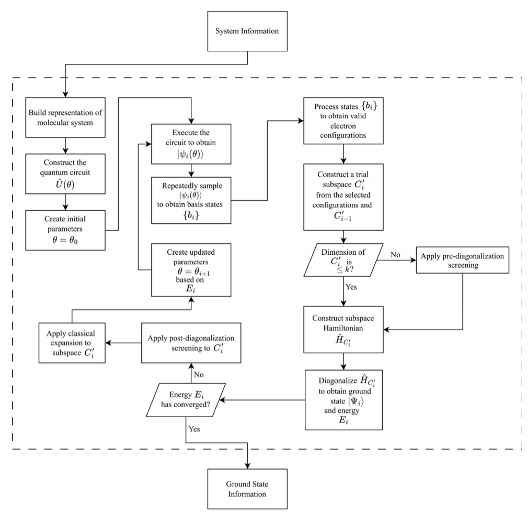
\includegraphics[width=\textwidth]{fig/HIVQE_paper.png}
    \caption{논문의 모식도}
    \label{fig:first}
  \end{subfigure}
  \hfill
  \vrule width 1pt  % 수직선 추가 (굵기: 1pt)
  \hfill
  \begin{subfigure}[b]{0.45\textwidth}
    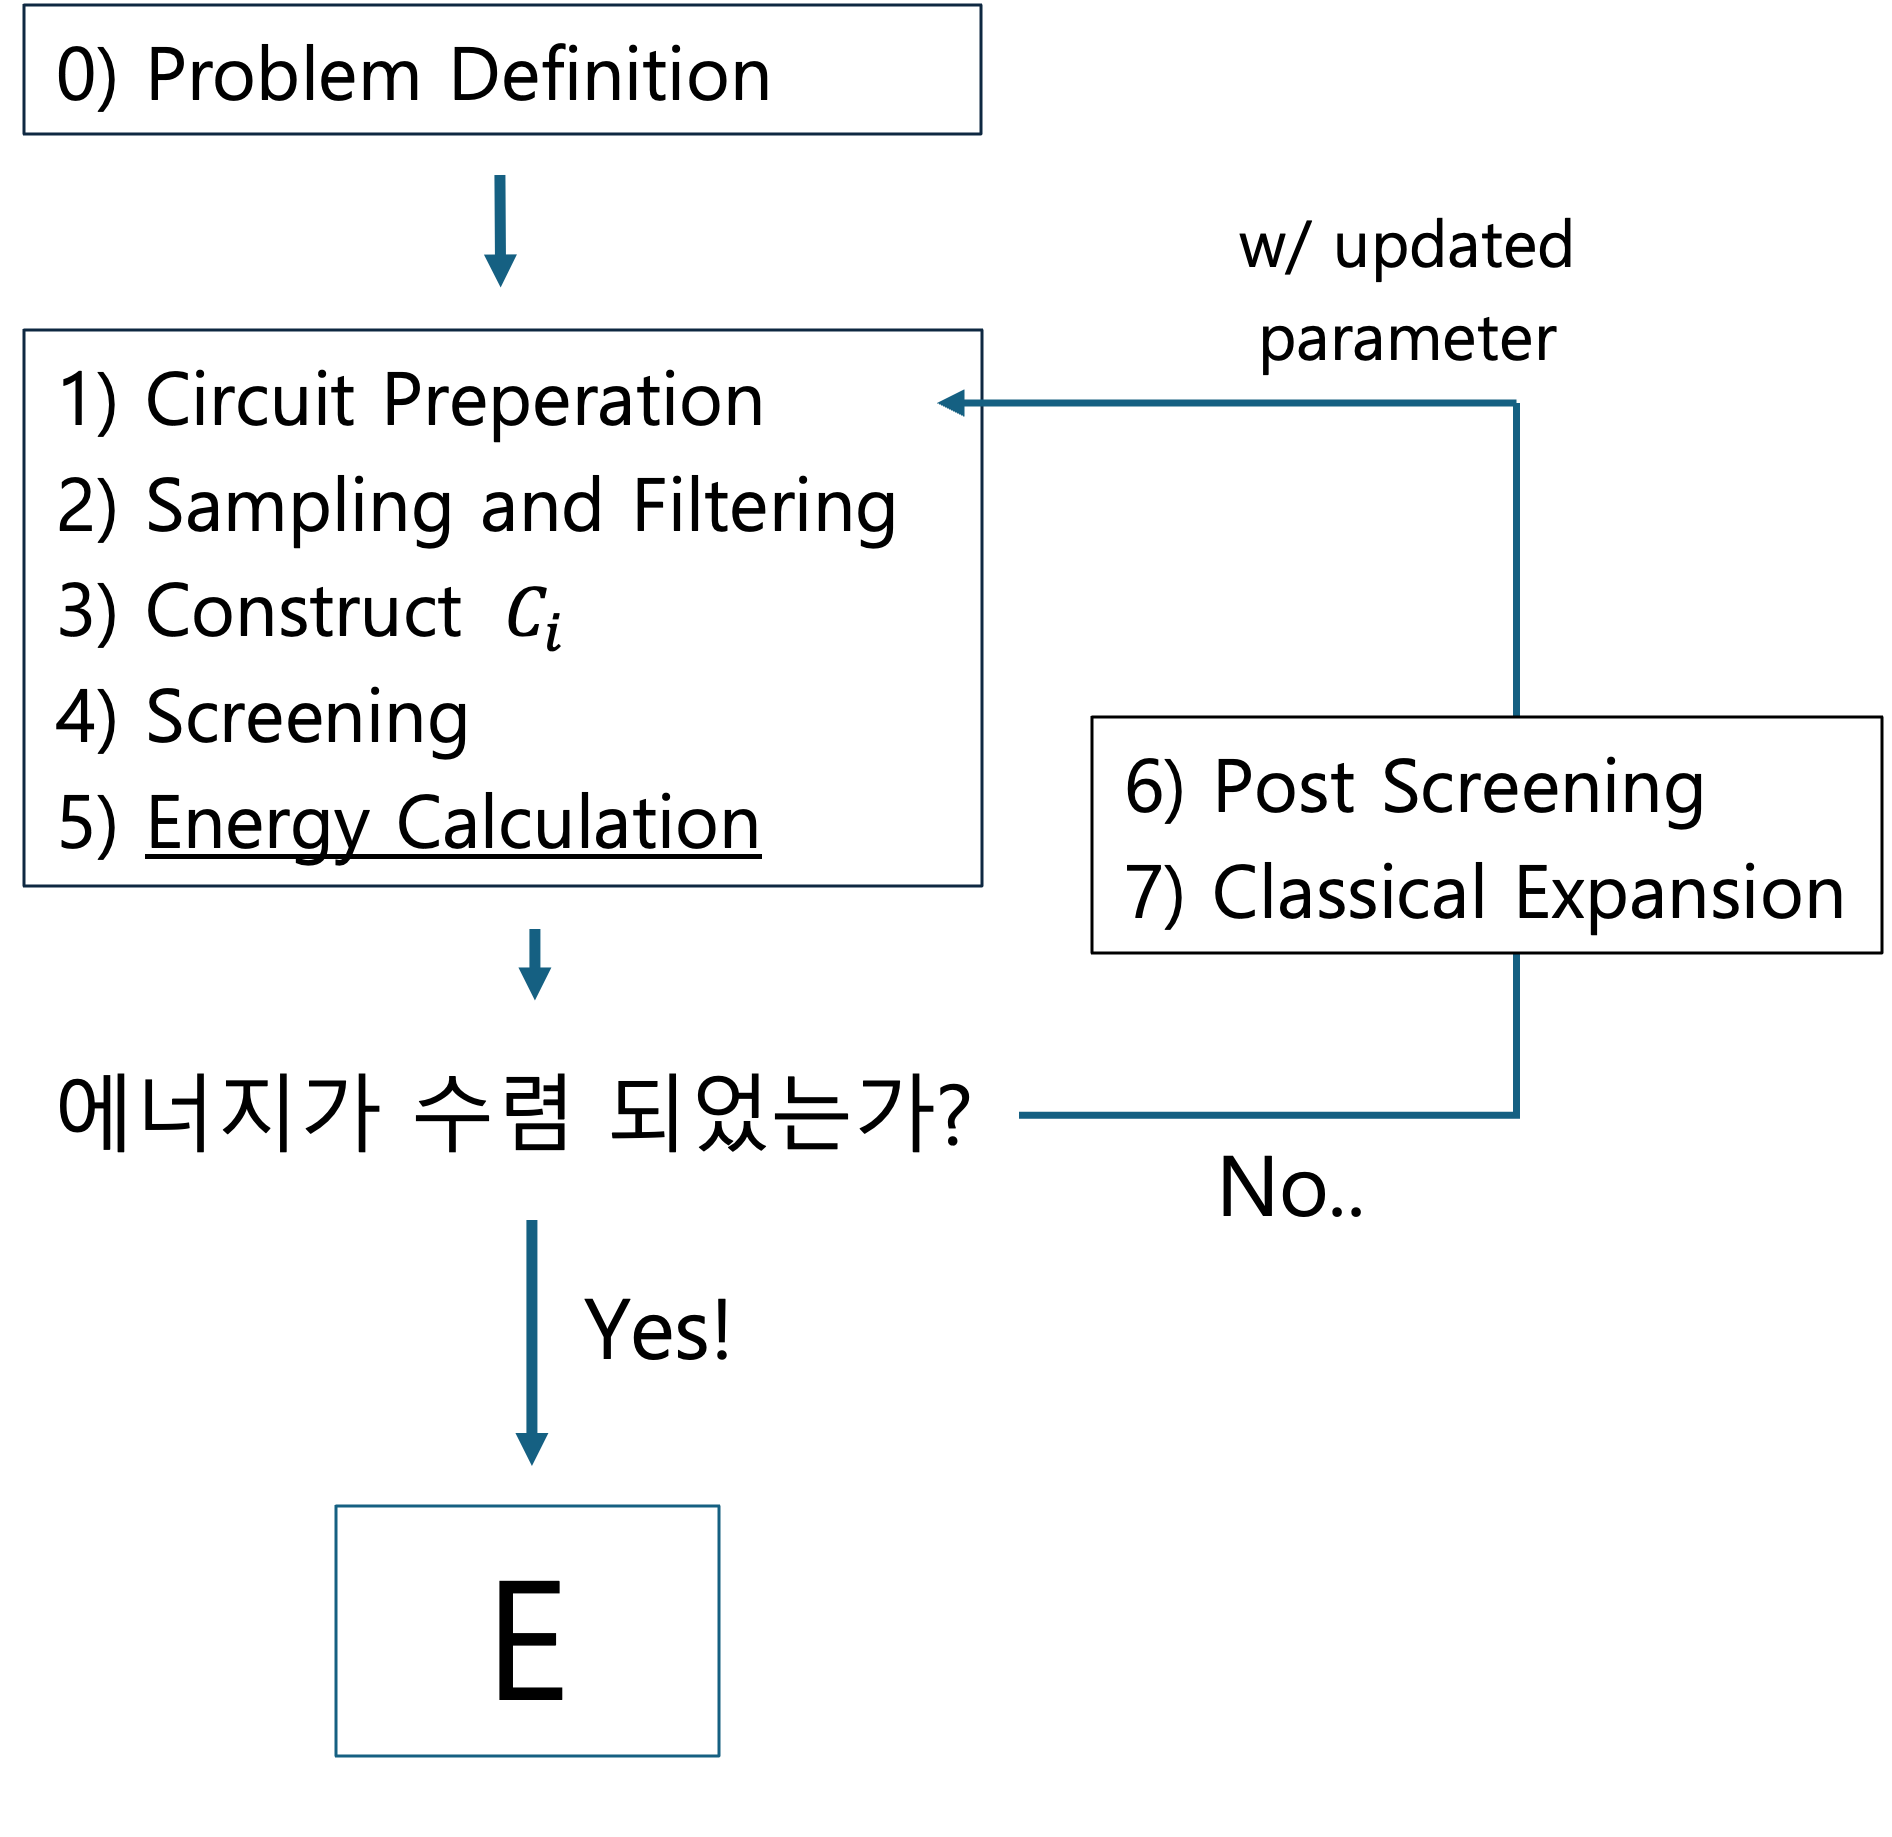
\includegraphics[width=\textwidth]{fig/HIVQE_my.png}
    \caption{내가정리}
    \label{fig:second}
  \end{subfigure}
  \caption{HIVQE pipeline}
  \label{fig:two_figures_side_by_side}
\end{figure}
여기서 헷갈릴 수 있는것은 계산의 흐름에서 3개의 사전지정 파라미터\(\left(k,\epsilon, m \right)\)가 나왔고, 그 3가지는 모두 다른 역할을 한다는것을 헷갈리면 안된다.

\newpage

\section{Result}
여러 분자에 대해서 실혐한 결과들을 나열해볼것이다. 정말로 각 시스템이 무엇인지는 사실 중요하지 않고, 우리가 볼것은 각 시스템의 Symmetric Space 의 차원이 몇이고, 우리의 계산에서는 몇개의 Basis 만을 사용했는지 (k) 가 중요하다. 
Symmetric Space 의 차원은 결국 FCI 계산을 위해 필요한 Slater Determinant의 개수를 의미하고, k값은 HIVQE 계산에서 필요한 Slater Determinant의 개수를 의미한다. 
즉, k 값이 Symmetric Space의 차원과 비슷해질 수록 FCI 계산에 가까워지며 Cost가 높아지지만 정밀도가 높아진다. 
여기서 보고자 하는것을 k값이 작더라도 화학적 정밀도를 유지 할 수 있는지를 확인해볼것이다. 
계산과정과 결과의 그래프에 대한 설명을 간단히 남기자면, 에너지의 계산결과는 FCI 보다 에너지가 낮게 나올 수는 없으므로, 오차는 양수일것이고, 이를 이후 Log 스케일로 그리기 위해 \(10^{-7}\) 이하의 오차는 모두 \(10^{-7}\) 로 plot 하였다.
그리고 사용하는 Cobyla 이외에도 3개의 iteration의 에너지 차이 이하라면 최적화 과정을 종료한다는 조건을 주었다. 이는 에너지 계산과정에 Sampling 과정이 들어있어, 이에의해 최적화과정이 제대로 수렴하지 못 할 가능성을 고려하였다. 

\subsection{\(H_2\) (\# of Electron : 2, \# of spin orbital : 4)}
\begin{figure}[H]
  \centering
  \begin{subfigure}[b]{0.45\textwidth}
    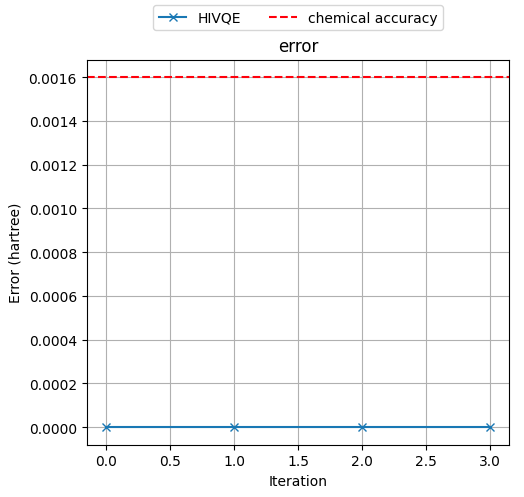
\includegraphics[width=\textwidth]{fig/H2_E}
    \caption{Energy Calc accuracy}
    \label{fig:first}
  \end{subfigure}
  \hfill
  \vrule width 1pt  % 수직선 추가 (굵기: 1pt)
  \hfill
  \begin{subfigure}[b]{0.45\textwidth}
    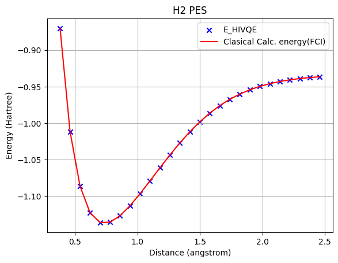
\includegraphics[width=\textwidth]{fig/H2_PES}
    \caption{Potential Energy Surface}
    \label{fig:second}
  \end{subfigure}
  \caption{H2 HIVQE Calculation}
  \label{fig:two_figures_side_by_side}
\end{figure}
\begin{center}
\textbf{number of Qubits : 4}\\
\textbf{Dimension of Symmetric Space:\(\binom{2}{1}\cdot\binom{2}{1}=4\)}\\
\textbf{k = 3}
\end{center}

왼쪽의 그림 (a) 는 Dist = 0.735 에서 \(H_2\)의 바닥상태 에너지를 계산하여 FCI 값과 비교하여 그린 그래프이다. 파란색 선은 HIVQE 의 계산결과와 FCI의 계산결과의 차이를 그린 그림이며, 
빨간선은 화학적 정밀도 \( \left(1.4 mHa\right)\) 를 나타낸 그림이다. 
모든 오비탈이 닫혀있으므로 이경우는 Singlet 이고, 따라서 upspin 와 downspin에 대응되는 전자와 스핀오비탈의 개수가 같다. 
따라서, Symmetric space 의 차원은 4이다. 이때 k 값은 3이였다. 즉, 전체 dimension의 75\% 만 사용하여 에너지를 계산하였고, 이때 3번의 iteration만에 수렴하였으며, 화학적 정밀도 이내의 정밀한 계산을 수행하였다. 
오른쪽의 그림 (b) 는 소위 PES(Potential Energy Surface)로, 거리를 변화시켜가며 에너지를 계산하여 plot한 그림이다. 빨간색 선은 FCI 를 통해 계산한 결과이며, 파란색은 HIVQE 를 통해 계산한 결과이다. 이경우도 모두 FCI 와 같은
결과를 보여주고 있음을 확인할 수있다. 
이 실험으로 HIVQE 알고리즘의 분자의 바닥상태 에너지를 정밀하게 계산할 수 있음을  확인했다. 하지만, 우리가 알고싶은것은, 이 HIVQE가 과연 큰 시스템에서도 정확하게, 그리고 효율적으로 에너지를 계산할 수 있는가 이다. 
그래서 이후에는 더 큰 시스템에 대해서 다뤄볼것이다. 

\subsection{\(LiH\) (\# of Electron : 4, \# of spin orbital : 12)}
\begin{figure}[H]
  \centering
  \begin{subfigure}[b]{0.25\textwidth}
    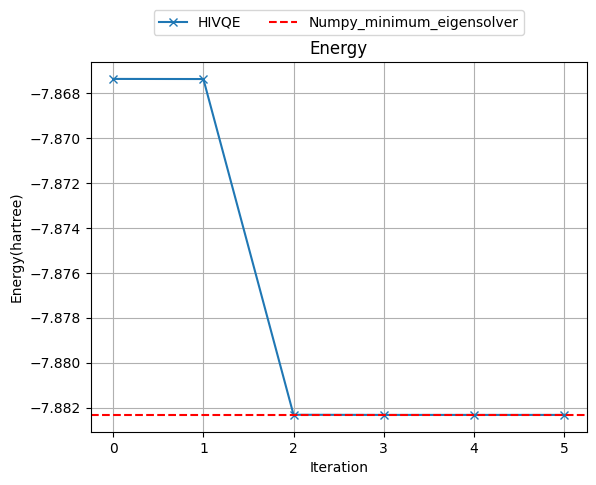
\includegraphics[width=\textwidth]{fig/LiH_E.png}
    \caption{Energy Calc}
    \label{fig:first}
  \end{subfigure}
  \hfill
  \vrule width 1pt  % 수직선 추가 (굵기: 1pt)
  \hfill
  \begin{subfigure}[b]{0.40\textwidth}
    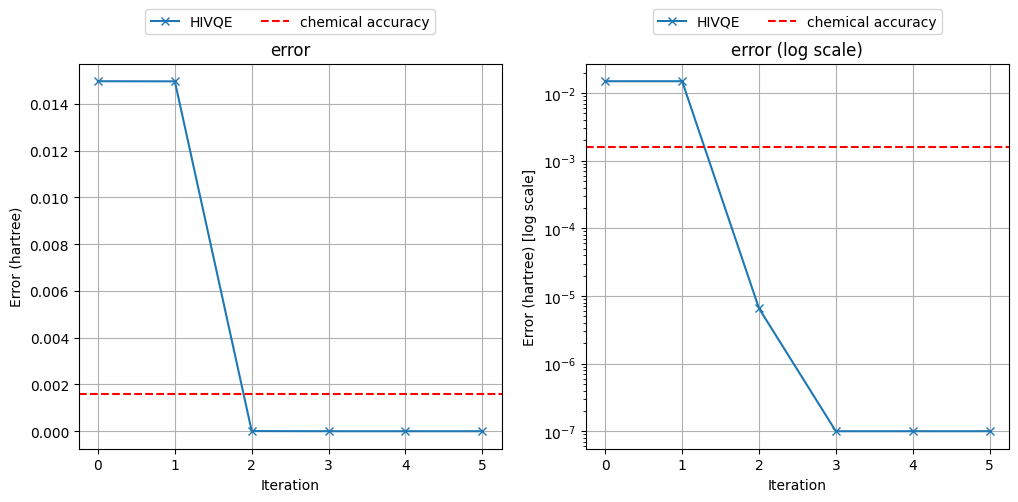
\includegraphics[width=\textwidth]{fig/LiH_dE.png}
    \caption{Energy Calc accuracy}
    \label{fig:second}
  \end{subfigure}
  \hfill
  \vrule width 1pt  % 수직선 추가 (굵기: 1pt)
  \hfill
  \begin{subfigure}[b]{0.25\textwidth}
    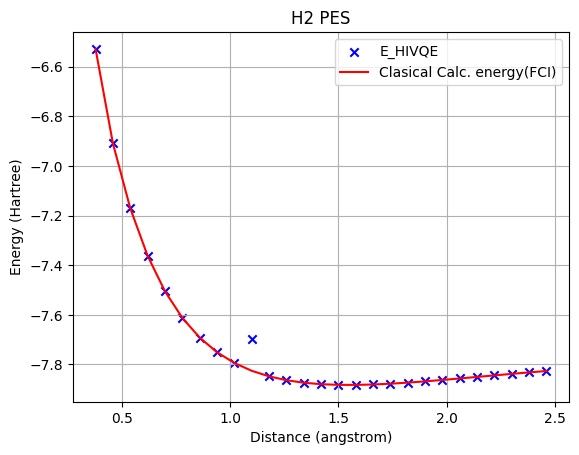
\includegraphics[width=\textwidth]{fig/LiH_PES.png}
    \caption{PES}
    \label{fig:second}
  \end{subfigure} 
  \caption{LiH HIVQE Calculation}
  \label{fig:two_figures_side_by_side}
\end{figure}
\begin{center}
\textbf{number of Qubits : 12}\\
\textbf{Dimension of Symmetric Space:\(\binom{6}{2}\cdot\binom{6}{2}=225\)}\\
\textbf{k = 100}
\end{center}
이번에는 에너지의 값 자체도 같이 그린 그래프를 추가하였다.
한가지 의문이 들 수 있는것은, 두 원자의 오비탈 점유를 표현해보면 H 는 \((1s)^{1}\) 이고, Li 는 \((1s)^{2}(2s)^{1}\) 니까 스핀오비탈이 6개여야 할 것 같은데 왜 스핀오비탈이 12개냐 이다.
이는 이러한 계산에 있어서 더 정밀한 계산을 위해서는 Virtual orbital, 즉 전자가 점유하지는 않지만, 전자가 \underline{점유할 수 있는} 오비탈도 고려해야 한다는것이다. 따라서 이경우는 Li 원자의 \(2p\) 오비탈 까지 고려하여 
조금 더 정밀한 계산을 시도하였기 때문에 총 6개의 Spartial orbital을 가지며 즉 12개의 Spin orbital 을 가진 시스템을 시뮬레이션 하였다. 
그림 (a)는 고정된 Dist 에서 Iteration 별로 계산된 에너지를 그린것이고, 파란색은 HIVQE, 빨간선은 그림에는 옵션을 수정하지 않아 Numpy Minimum Eigensolver라고 되어있지만, FCI 값이다. 
당연히 FCI 값은, Iteration별로 변하지 않으므로 상수이다. 최적화 과정이 진행되며 FCI 값과 비슷한 값이 됨을 볼 수 있으며 다음 그림을 통해 정확한 차이를 볼 수 있다. 
그림 (b)는 HIVQE와 FCI의 계산결과의 차이를 왼쪽에는 Hartree 단위, 오른쪽에는 Log 스케일로 그림을 그린것이며, 파란색은 HIVQE 와 FCI의 차이, 그리고 빨간선은 화학적 정밀도 \(1.3mHa\) 이다. 
2번에 Iteration 안에 화학적 정밀도 이내로 떨어졌고, 최종 결과 또한 화학적 정밀도 이내로 계산하였음을 알 수 있다. 
그림 (c)는 거리별로 옵션을 변화시켜가며 에너지를 계산하여 그린 PES 이다. 빨간색은 FCI의 계산결과이며, 파란색은 HIVQE의 계산결과이다. 
한 군데 튀는값이 있는데, 이 원인은 정확히는 모르겠으나, 추측컨데 최적화 과정이 제대로 되지 않은것이라 판단할 수 있다. 
실험당 걸린 시간은 하나의 거리에 대해서, 즉 (a), (b) 그림을 얻는 계산에서 약 10분정도 소요되었다. 이는 기존의 VQE 보다는 더 짧은 시간이다. 
총 12개의 큐비트를 사용하는 시스템도 정확히 시뮬레이션 할 수 있음을 확인할 수 있었다. 다음 시스템으로 넘어가보자. 

\subsection{\(H_2O\) (\# of Electron : 10, \# of spin orbital : 14)}
\begin{figure}[H]
  \centering
  \begin{subfigure}[b]{0.3\textwidth}
    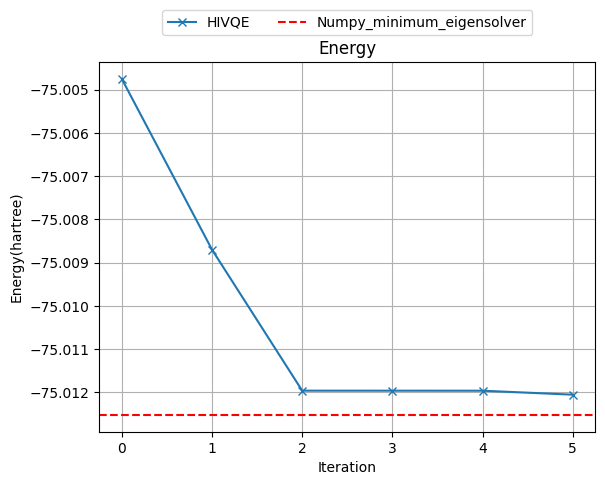
\includegraphics[width=\textwidth]{fig/H2O_E.png}
    \caption{Energy Calc}
    \label{fig:first}
  \end{subfigure}
  \hfill
  \vrule width 1pt  % 수직선 추가 (굵기: 1pt)
  \hfill
  \begin{subfigure}[b]{0.6\textwidth}
    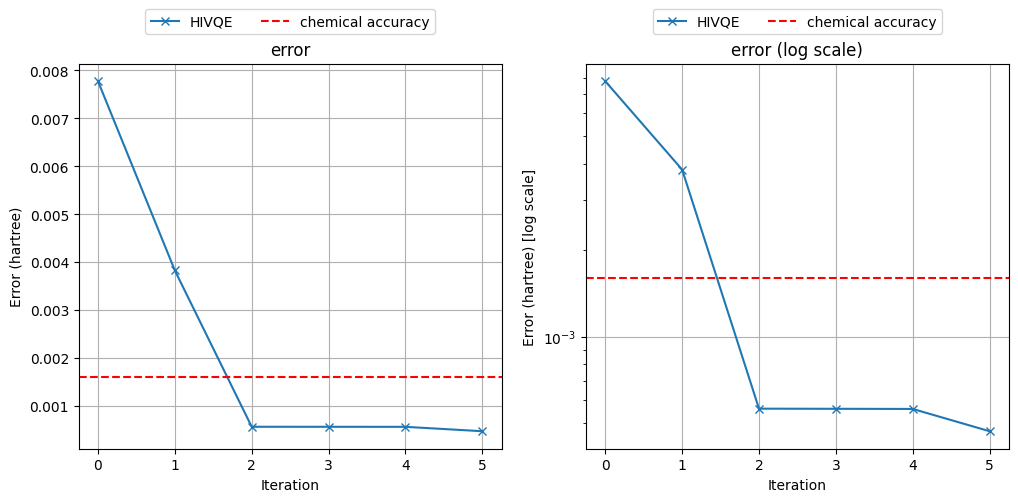
\includegraphics[width=\textwidth]{fig/H2O_dE.png}
    \caption{Potential Energy Surface}
    \label{fig:second}
  \end{subfigure}
  \caption{H2O HIVQE Calculation}
  \label{fig:two_figures_side_by_side}
\end{figure}
\begin{center}
\textbf{number of Qubits : 14}\\
\textbf{Dimension of Symmetric Space:\(\binom{7}{5}\cdot\binom{7}{5}=441\)}\\
\textbf{k = 150}
\end{center}
k 값을 올리니 이경우에는 한 계산에서 약 1시간정도 걸려서 PES 를 그리기는 힘들어 그리지않았다. 특히 H2O의 경우 각도도 변화시켜 그림을 그려야하기 때문에 더 걸리게될것이다. 
이번에는 각 원자의 오비탈 점유를 표현해보면 H 는 \((1s)^{1}\) 이고, O 는 \((1s)^{2}(2s)^{2}(2p)^{4}\) 여서 총 스핀오비탈이 14개가 된다. 
마찬가지로 (a)는 에너지의 계산결과, (b)는 에너지의 오차이다. 
H2O 까지도 효과적으로 에너지를 계산 할 수 있다. 이정도 계산에서는 효과적으로 에너지를 계산할 수있음을 확인했으니, 우리가 기존에 다루던 LiCoO2의 분자에 대해서 다뤄보자.

\subsection{\(LiCoO2\) (FMO)}
우리가 기존의 LiCoO2 에서 아주정확한 결과를 내지 못한 이유에서 메인이 되는이유는 FMO 방식에서도 있었지만, 각 Fragment 에서의 VQE도 최적화 과정에 인한 오차가 있었다. 
만약 HIVQE를 통해 각 Fragment의 에너지를 잘 계산해 낸다면, 뭔가 다른 이야기를 할 수 도 있을것이다. FMO 방식에 대해서 간단하게만 이야기 하자면, LiCoO2 분자는 아래의 그림 (a)와같이 생겼는데, 
이를 통째로 다루기에는 그 시스템이 너무 크기때문에 오른쪽의 각각 조각으로 쪼개서 에너지를 계산하고 이를 적절한 방식을 이용해서 합치자는것이다. 
\begin{figure}[H]
  \centering
  \begin{subfigure}[b]{0.3\textwidth}
    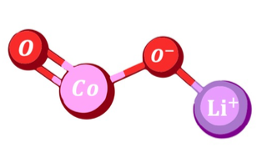
\includegraphics[width=\textwidth]{fig/LiCoO2.png}
    \caption{LiCoO2 diagram}
    \label{fig:first}
  \end{subfigure}
  \hfill
  \vrule width 1pt  % 수직선 추가 (굵기: 1pt)
  \hfill
  \begin{subfigure}[b]{0.6\textwidth}
    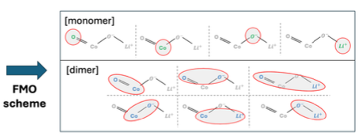
\includegraphics[width=\textwidth]{fig/LiCoO2_FMO.png}
    \caption{Fragment}
    \label{fig:second}
  \end{subfigure}
  \caption{LiCoO2 FMO diagram}
  \label{fig:two_figures_side_by_side}
\end{figure}

일단 monomer에 대해서는 에너지를 계산할 수 있을것 같으니, 테스트해보고 싶은것은 Dimer 에 대해서 이다. 
\subsubsection{Li-O Dimer (near, far)(\# of Valence Electron : 5, \# of Valence spin orbital : 8)}
여기서 부터는 다른 Fragment들과의 일관성을 위해 모두 Active Space 를 다루기 때문에, 최외곽의 전자와 스핀오비탈에 대한 정보가 중요하다. 
Active Space 란 결국 헤밀토니안은 생성과 소멸 연산자로 이루어져있으며, VQE를 통해 에너지를 계산 하고자하는것은 이들간의 잘 모르는 Dynamics를 보고자 하는것인데, 
각 원자의 Core 오비탈은 보통 결합에 참여하지 않고, 그 자체로 존재할것이기 때문에 그 Dynamics를 상수로 볼 수 있을것이다. 그래서, 이러한 Core orbital에 대해서 
VQE를 통해 계산하지 않고, 따로 상수로써 계산하여 문제를 해결하는데에 필요한 큐비트 수를 줄이는 전략이 Active Space 방식이다. 
이경우를 보자면, Li의 \((1s)^{2}\) 의 오비탈과 O의 \((1s)^{2}(2s)^{2}\) 오비탈을 Core 오비탈로 하여 VQE 로 계산해야하는 Spin orbital을 총 6개 줄일 수 있다. 
저 위에 그림 19-(b) 를 보면, Li-O 의 구성을 갖는 Dimer는 총 2개이다. 이 2개에 대해서 에너지를 계산해본 결과를 볼것이다. 
\begin{figure}[H]
  \centering
  \begin{subfigure}[b]{0.45\textwidth}
    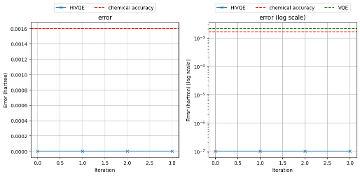
\includegraphics[width=\textwidth]{fig/LiO_far.png}
    \caption{LiO Dimer(far)}
    \label{fig:first}
  \end{subfigure}
  \hfill
  \vrule width 1pt  % 수직선 추가 (굵기: 1pt)
  \hfill
  \begin{subfigure}[b]{0.45\textwidth}
    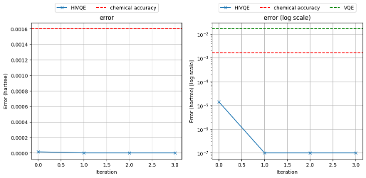
\includegraphics[width=\textwidth]{fig/LiO_near.png}
    \caption{LiO Dimer(near)}
    \label{fig:second}
  \end{subfigure}
  \caption{Li-O Energy calc}
  \label{fig:two_figures_side_by_side}
\end{figure}

\begin{center}
\textbf{number of Qubits : 8}\\
\textbf{Dimension of Symmetric Space:\(\binom{4}{3}\cdot\binom{4}{2}=24\)}\\
\textbf{k = 150}
\end{center}
여기서부터는 이제 닫혀있는 시스템이 아니므로, upspin과 downspin의 개수가 달라지게 된다. 사실 이부분이 좀 깊게 고민을 해보았는데 아직까지 조금 애매한 부분이 있긴 하지만, 기존의 FMO/VQE 에서 다루던대로 다루어보겠다.
그림 (a)는 두 원자가 멀리 떨어져있는 Dimer, 그림(b)는 두 원자가 가깝게 있는 Dimer 이다. 이 맥락에서 이 FMO에 관한 디테일한 내용은 다룰 필요가 없으니, 그냥 구성은 갖지만 기하학적인 구조가 다른 두 시스템 이라고 생각하자. 
각 그림에서 왼쪽은 Ha 단위로, 파란색이 Iteration별로 HiVQE를 통해 계산된 에너지와 Numpy Minimum Eigensolver로 계산된 에너지의 차이이고, 그리고 빨간색이 화학적 정밀도를 표시해둔것이다. 
그리고 각그림에서 오른쪽은 이전의 오차를 log 스케일로 표현해둔것이며, 초록색으로 VQE를 통해 계산된 에너지의 정밀도 또한 표현하였다. 
기존에 VQE에서는 화학적 정밀도에는 도달하지 못했지만, HIVQE 에서는 화학적 정밀도이상으로 정확하게 계산해낸것을 확인 할 수 있다. 
사실 애매한 부분이 여기에 있는데, 이경우는 Dimension of Symmetric Space 가 24 이다. 즉, 내가 k값을 30으로 했다는것은 쓸데없는 6개의 Slater Determinant를 포함하여 FCI 를 계산한것이라 당연히 정확하게 나온게 맞는데, 
과연 저렇게 계산한게 맞는가? 하는 생각은 있다. 그래서 이 FMO를 다루려면 저렇게 닫혀있지 않은 시스템을 다루는 방법에 대한 논의가 필요한데, 이부분이 다룰수록 애매해지는것 같다. 
일단은, 특정 시스템에 대해서 VQE보다 정확하게 에너지를 계산해내었다 정도만 이해하고 넘어가자. 

\subsubsection{O-O Dimer (\# of Valence Electron : 8, \# of Valence spin orbital : 12)}
\begin{figure}[H]
  \centering
  \begin{subfigure}[b]{0.5\textwidth}
    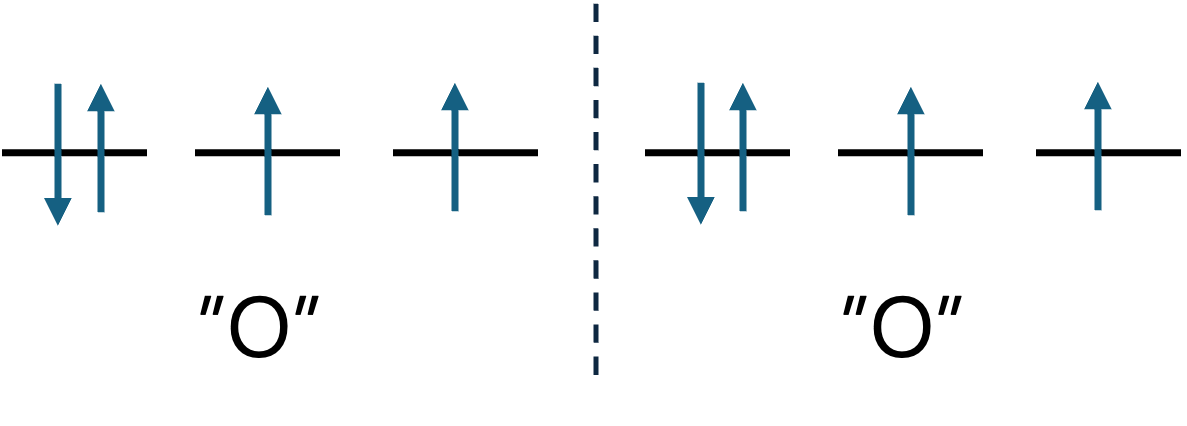
\includegraphics[width=\textwidth]{fig/OO_conf.png}
    \caption{O-O Configuration}
    \label{fig:first}
  \end{subfigure}
  \hfill
  \vrule width 1pt  % 수직선 추가 (굵기: 1pt)
  \hfill
  \begin{subfigure}[b]{0.4\textwidth}
    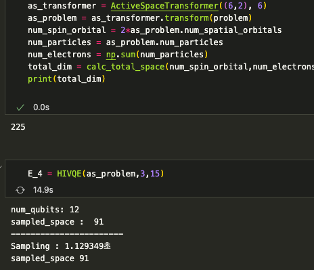
\includegraphics[width=\textwidth]{fig/OO_exp.png}
    \caption{LiO Dimer(near)}
    \label{fig:second}
  \end{subfigure}
  \caption{O-O experiment}
  \label{fig:two_figures_side_by_side}
\end{figure}
\begin{center}
\textbf{number of Qubits : 12}\\
\textbf{Dimension of Symmetric Space:\(\binom{6}{6}\cdot\binom{6}{2}=15\)}\\
\textbf{k = ??}
\end{center}
분명 Symmetric Space의 정의대로, 계산해보면, 그림(a)에서 보이는것이 서로 결합하지 않은 O-O 가 보일 수 있는 Configuration 일것인데, 저렇게 조건을 주게되면, 차원이 15로 계산된다. 
그런데 샘플링되는 상태의 수가 Symmetric space의 차원보다 크게된다. 그래서 이러한 열린상황에서는 다른 논리가 필요하다는것을 느껴 실험을 약간 다르게 세팅하였다. 
spin에 해당하는 정보가 필요했던건, 계산에 필요했던 basis의 갯수를 줄이기 위함이였다. 따라서 spin에 해당하는 제약을 없애더라도, 계산의 정밀도 자체는 변하지 않는다. 
계산이 진행되는 흐름이 계속해서 낮은 에너지를 갖는 Slater Determinant를 찾는것이므로, 최적화 과정에서 알아서 적절한 Spin에 해당하는 Configuration을 찾아줄 것이다. 
일단 지금까지의 실험에서는 UCCSD ansatz를 사용하였고, 그렇게되면, 앞서말했던 전자수와 스핀에 해당하는 정보가 Ansatz에도 들어있게된다. 그래서 이후로는 twolocal Anstz를 이용해서 계산을 수행한다. 
그렇게 계산된 결과가 아래와같다. 

\begin{figure}[H]
  \centering
  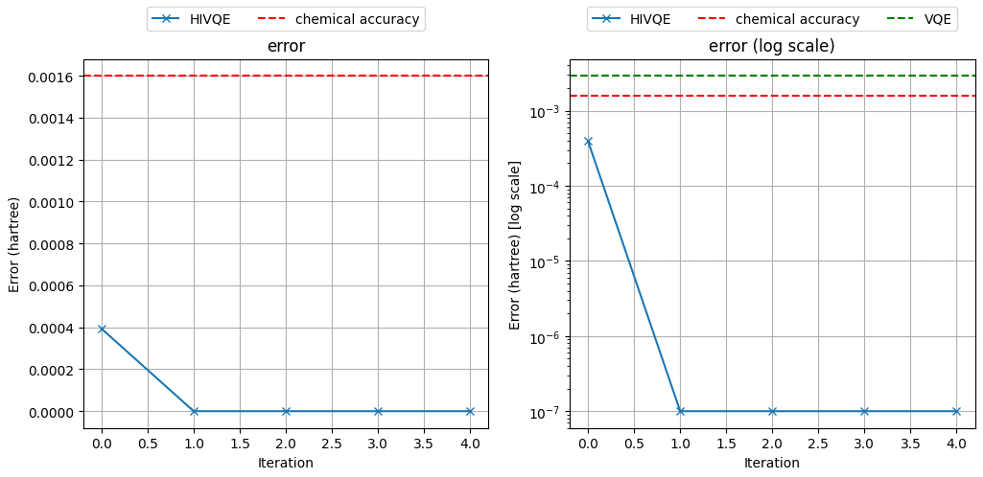
\includegraphics[width=0.8\textwidth]{fig/OO_EE.png}
  \caption{O-O Energy Calculation}
  \label{fig:first}
\end{figure}
마찬가지로 왼쪽 그림이 Hartree 단위로 HIVQE 의 결과와 Numpy Minimum Eigensolver 의 오차를 그린 그림이고, 오른쪽 그림이 Log scale로 VQE의 결과까지 포함하여 그린 그림이다. 
이경우도 마찬가지로 화학적 정밀도 이내의 정밀도로 계산을 해낼 수 있었다. 

\subsubsection{Co-Li Dimer (\# of Valence Electron : 8, \# of Valence spin orbital : 12)}
\begin{figure}[H]
  \centering
  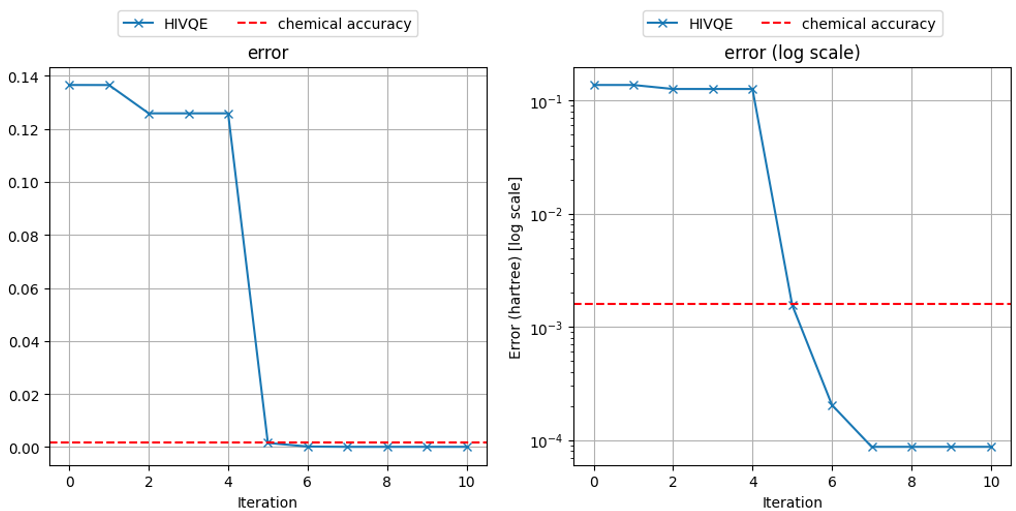
\includegraphics[width=0.8\textwidth]{fig/Co-Li.png}
  \caption{Co-Li Energy Calculation}
  \label{fig:first}
\end{figure}
twolocal을 사용하니 확실히 시작점 에서의 오차가 커지게된다. 
일단 왼쪽그림은 이번에는 Hartree 단위로 파란색은 HIVQE 의 결과, 빨간색은 Numpy Minimum Eigensolver의 결과를 나타낸다.
그리고 오른쪽 그림은 둘의 오차를 log 스케일로 그린 그림이다. 마찬가지로 화학적 정밀도 이내의 계산을 수행하였다. 
이제 다음순서는 Co-O Dimer 두개의 에너지를 계산하는것이 순서이지만, 이렇게 계산이 되는걸 보니 LiCoO2를 통째로 계산하는것도 가능하지 않을까? 라는 생각이 들었다. 
그렇게 하게되면 LiCoO2 분자는 닫혀있기 떄문에 Spin에 관한 고민을 하지 않아도 되고, 여기서 테스트 해보는것이 실제 논문에서 다룬 시스템의 크기와 비슷한 정도라 오히려 그것이 합리적으로 보였다. 

\subsection{\(LiCoO2\) (total) (\# of Valence Electron : 12, \# of Valence spin orbital : 24)}
\begin{figure}[H]
  \centering
  \begin{subfigure}[b]{0.6\textwidth}
    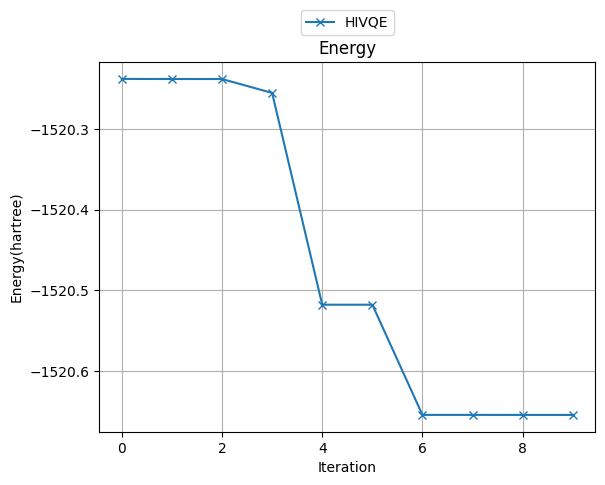
\includegraphics[width=\textwidth]{fig/LiCoO2_tot.png}
    \caption{LiCoO2 total Energy Calculation}
    \label{fig:first}
  \end{subfigure}
  \hfill
  \vrule width 1pt  % 수직선 추가 (굵기: 1pt)
  \hfill
  \begin{subfigure}[b]{0.3\textwidth}
    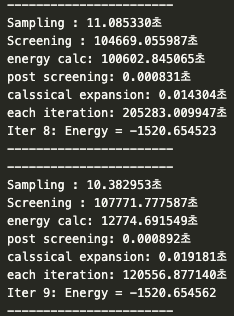
\includegraphics[width=\textwidth]{fig/tot_exp.png}
    \caption{experiment time}
    \label{fig:second}
  \end{subfigure}
  \caption{LiCoO2 calc}
  \label{fig:two_figures_side_by_side}
\end{figure}

\textbf{number of Qubits : 24}\\
\textbf{Dimension of Symmetric Space:\(\binom{12}{6}\cdot\binom{12}{6}=853776\)}\\
\textbf{k = 2000}
확실히 시스템이 커지니 Symmetric Space 가 커진다. 그리고 계산 소요시간도 거의 1주일 정도 걸리게된다. 
그리고 수렴이 된 값을 확인해보니, 같은 Active Space 조건을 부여한 FCI 에 비해서는 훨씬 정확하지 않다. 이 원인은 k값을 너무 작게 잡았기 때문이다. 
하지만 에너지의 계산이 충분히 진행되는것을 보아, 서버컴퓨터를 활용해 더 높은 k값을 주어 에너지를 계산하면 정확한 에너지를 계산할 수 있음을 기대해볼 수 있다. 

\section{Conclusion}
HIVQE 에 관해 필요한 기초지식들과 실제로 적용한 방식들에 대해서 다루고, 실험 결과 데이터도 같이 다루었다. 
분명 이 알고리즘은 정밀하게 시스템의 바닥상태 에너지를 계산해 내는것을 확인 할 수 있다. 하지만, 이게 과연 양자적 현상을 이용해 발전한 양자알고리즘이 맞나? 라는생각이 계속해서 들었다. 
일단 계산에 있어서도 대부분의 계산소요시간은 고전컴퓨터에서 소모하게 되고 실제 양자회로를 사용하는것은 Sampling과정밖에 없다. 
시스템의 CI류 계산에 필요한 Determinant의 개수는 시스템의 크기에 Exponential 하게 커진다. 논문에서도 전체 시스템의 차원이 2\% 정도를 사용했을때 소위말하는 화학적 정밀도를 얻었다고했는데, 
그럼 계산에 필요한 Determinant의 개수를 \(\frac{1}{50}\) 정도로 줄인건데, 이러한 계산이 과연 시스템이 더욱 커질때에도 유효할지는 사실 논리적으로 봤을때 그렇지 않을 가능성이 높아보인다. 
하지만 그럼에도 기존의 VQE로 다루는것 보다는 더 적은 시간에 더 좋은 정밀도로 계산한것은 사실이긴했다. 과연 더 큰시스템에서도 잘 계산할지에 관해서는 서버컴퓨터를 활용하면서 논문의 결과를 같이 얻어보면서 테스트 해보고자 한다. 
\subsection{Future Work}
일단 추가로 더 큰 시스템에 대해서 잘 작동하는지를 테스트 해보아야하고, 열린시스템에서 spin의 옵션을 어떻게 주어야할지, 그리고 CI 계산에 필요한 논리인 Slater Determinant 집합 시스템의 anti-Symmetric 공간을
Span 하는지에 대해서 조금 더 공부해보아야 할것이다. 
\end{document}
